\documentclass
[   oneside,         % oneside/twoside : Einseitiger oder zweiseitiger Druck?
    12pt,            % Bezug: 12-Punkt Schriftgre
    DIV15,           % Randaufteilung, siehe Dokumentation "KOMA"-Script
    BCOR17mm,        % Bindekorrektur: Innen 17mm Platz lassen. Copyshop-getestet.
    headsepline,     % Unter Kopfzeile Trennlinie (aus: headnosepline)
    footsepline,     % ber Fuzeile Trennlinie (aus: footnosepline)
    openright,       % Neue Kapitel im zweiseitigen Druck rechts beginnen lassen
    a4paper,         % Seitenformat A4
    abstracton,      % Abstract einbinden
	english,
    listof=totoc,version=first,      % Div. Verzeichnisse ins Inhaltsverzeichnis aufnehmen
    bibliography=totoc,version=first,        % Literaturverzeichnis ins Inhaltsverzeichnis aufnehmen
    titlepage,       % Titelseite aktivieren
    headinclude,     % Seiten-Head in die Satzspiegelberechnung mit einbeziehen
    footexclude,     % Seiten-Foot nicht in die Satzspiegelberechnung mit einbeziehen
    numbers=noenddot,version=first % Gliederungsnummern ohne abschlieenden Punkt darstellen
]   {scrreprt}       % Dokumentenstil: "Report" aus dem KOMA-Skript-Paket

\usepackage[active]{srcltx}
%\usepackage[activate=normal]{pdfcprot\documentclass[options]{class}} % Optischer Randausgleich -> pdflatex!
\usepackage{ifthen}
\usepackage[english,ngerman]{babel}
%\usepackage[english]{babel}
%\usepackage{ngerman}
%\usepackage[fixlanguage]{babelbib}
%\setbiblanguage{english}
\usepackage[latin1]{inputenc}
\usepackage[T1]{fontenc}
\usepackage[T1]{url}
\usepackage{ae}
\usepackage[final]{graphicx}
\usepackage[automark]{scrpage2}
\usepackage{setspace}
\usepackage{floatflt} 
\usepackage{rotating} 
\usepackage{wrapfig}
%\usepackage{subfig}
\usepackage{graphicx}
%\usepackage[first,light]{draftcopy} % Fr Probedruck
\usepackage[plainpages=false,pdfpagelabels,hypertexnames=false]{hyperref}
\usepackage{pdfpages}	%include pdf files
\usepackage{listings} %include sourcecode
\usepackage{color}
\definecolor{commentgreen}{rgb}{0,0.5,0}
\usepackage{multirow}
\usepackage{verbatim}
\usepackage{amsmath}
\usepackage{amssymb}
\usepackage{amsfonts}
\usepackage{enumitem}
\usepackage{setspace}
\usepackage{array}
\usepackage{nomencl}
% \usepackage[table]{xcolor}
\usepackage{longtable}
\usepackage{url}
\usepackage{subcaption}
\usepackage{longtable}
%\usepackage{paralist}
\usepackage{tipa}

%\usepackage{textcomp}  %mit \textcent geht Cent-Symbol




% Tiefe der Kapitelnummerierung beeinflussen
\setcounter{secnumdepth}{3} % Tiefe der Nummerierung
\setcounter{tocdepth}{3}    % Tiefe des Inhaltsverzeichnisses

% Hier in die zweite geschweifte Klammer jeweils
% die persnlichen Daten eintragen:
%\newcommand{\artderausarbeitung}{PhD Thesis}
\newcommand{\artderausarbeitung}{}
%\newcommand{\namedesautors}{Anna Marie Kruspe}
\newcommand{\namedesautors}{}
\newcommand{\inventarisierungsnummer}{}

\newcommand{\markup}[1]{\textbf{#1}}

% Seitenlayout festlegen. Hier nichts ndern!
\pagestyle{scrplain}
\ihead[]{\headmark}
\ohead[]{\pagemark}
\chead[]{}
\ifoot[]{\scriptsize \inventarisierungsnummer}
\ofoot[]{\scriptsize \artderausarbeitung\ \namedesautors}
\cfoot[]{}
\renewcommand{\titlepagestyle}{scrheadings}
\renewcommand{\partpagestyle}{scrheadings}
\renewcommand{\chapterpagestyle}{scrheadings}
\renewcommand{\indexpagestyle}{scrheadings}

% Abschnittsweise Nummerierung anstatt fortlaufend. Hier nichts ndern!
\makeatletter
\@addtoreset{equation}{chapter}
\@addtoreset{figure}{chapter}
\@addtoreset{table}{chapter}
\renewcommand\theequation{\thechapter.\@arabic\c@equation}
\renewcommand\thefigure{\thechapter.\@arabic\c@figure}
\renewcommand\thetable{\thechapter.\@arabic\c@table}\makeatother

% Quelltextrahmen, klein. Hier nichts ndern!
\newsavebox{\inhaltkl}
\def\rahmenkl{\sbox{\inhaltkl}\bgroup\small\renewcommand{\baselinestretch}{1}\vbox\bgroup\hsize\textwidth}
\def\endrahmenkl{\par\vskip-\lastskip\egroup\egroup\fboxsep3mm%
\framebox[\textwidth][l]{\usebox{\inhaltkl}}}

% Quelltextrahmen, normale Groesse. Hier nichts ndern!
\newsavebox{\inhalt}
\def\rahmen{\sbox{\inhalt}\bgroup\renewcommand{\baselinestretch}{1}\vbox\bgroup\hsize\textwidth}
\def\endrahmen{\par\vskip-\lastskip\egroup\egroup\fboxsep3mm%
\framebox[\textwidth][l]{\usebox{\inhalt}}}


% Sonstige Befehlsdefinitionen hier ablegen.
\newcommand{\entspricht}{\stackrel{\wedge}{=}}
\definecolor{light-gray}{gray}{0.95}
\addto\captionsenglish{\renewcommand{\contentsname}{Table of Contents}}
%\makenomenclature
\makeglossary
\DeclareMathOperator*{\argmin}{argmin}
\DeclareMathOperator*{\argmax}{argmax}

\begin{document}
\onehalfspacing
\clubpenalty=10000
\widowpenalty=10000
\selectlanguage{english}
\thispagestyle{empty}
%Eigentlich f�r documentclass [11pt] ausgelegt!
\begin{center}
\large{Technische Universit�t Ilmenau}\\
\large{Fakult�t f�r Elektrotechnik und Informationstechnik}
\end{center}

\vspace{0.15cm}

%\begin{figure}[htbp]
%  \centering
%  \subfloat[]{
\includegraphics[width=0.4\textwidth]{images/tui_logo.pdf}}
%  \subfloat[]{\includegraphics[width=0.4\textwidth]{images/idmt_logo.pdf}}
%\end{figure}

\begin{figure}[htbp]
\begin{center}$
\begin{array}{cc}

\includegraphics[width=0.4\textwidth]{images/tui_logo} &

\includegraphics[width=0.4\textwidth]{images/idmt_85mm_p334}
\end{array}$
\end{center}
\end{figure}

\vspace{0.6cm}

\begin{center}
%\renewcommand{\baselinestretch}{1.50}\normalsize		%Zeilenabstand
%\vspace{0.25cm}
\textbf{\Large{Application of Speech Recognition Algorithms to Singing}}\\

%\renewcommand{\baselinestretch}{1.00}\normalsize
\end{center}
\vspace{.3cm}

\begin{center}
%Diplomarbeit am Fraunhofer Institut f�r Digitale Medientechnik
Doctoral Thesis
\end{center}






\vspace{3.0cm}
\begin{flushleft}
\small
\renewcommand{\arraystretch}{1.5} 
\begin{tabular}{lll}
\textbf{Submitted by:} & & Anna Marie Kruspe\\
\textbf{Submission date:} & & \\
\textbf{Course of study:} & & Media Technology\\
%\textbf{Specialisation:} & & Audio-Visual Technology\\
\textbf{Matriculation Number:} & & 39909 \\
& & \\
\end{tabular}
\begin{tabular}{lll}
%\textbf{Verantwortlicher Hochschullehrer:} & & Prof. Dr.-Ing. Karlheinz Brandenburg\\
\textbf{Advisor:} & & Prof. Dr.-Ing. Dr. rer. nat. h.c. mult. Karlheinz Brandenburg \\
%\end{tabular}
%\begin{tabular}{lll}
%\textbf{Faculty Advisors:}  & & Advisor 1 \\ & & Advisor 2 \\ & & Advisor 3\\
\end{tabular}
\end{flushleft}





% Inhaltsverzeichnis
\cleardoublepage % Seitenumbruch erzwingen vor nderung des Nummerierungsstils
\footnotesize
%\begin{otherlanguage}[english]
\pagenumbering{roman} % Nummerierung der Seiten ab hier: i, ii, iii, iv...
\pagestyle{scrheadings} % Ab hier mit Kopf- und Fusszeile

\normalsize
%\renewcommand{\abstractname}{Kurzfassung}
%\begin{otherlanguage}{english}
\begin{abstract}
The research field of Music Information Retrieval is concerned with the automatic analysis of musical characteristics. One aspect that has not received much attention so far is the automatic analysis of sung lyrics. On the other hand, the field of Automatic Speech Recognition has produced many methods for the automatic analysis of speech, but those have rarely been employed for singing so far. This thesis analyzes the feasibility of applying various speech recognition methods to singing, and suggests adaptations. In addition, the routes to practical applications for these systems are described. Five tasks are considered: Phoneme recognition, language identification, keyword spotting, lyrics-to-audio alignment, and retrieval of lyrics from sung queries.\\
For the task of phoneme recognition, two large data sets were created. The first one is generated by making speech recordings more ``song-like''. The second one is based on an existing singing data set with matching textual lyrics, which are automatically aligned to the audio and then used for training new acoustic models. The phoneme error rate is improved from $1.08$ to $0.77$ on singing.\\
Two methods for language identification are presented. The first one employs i-vector extraction and achieves an accuracy of $0.73$ on singing. The second method is a completely new approach based on the extraction of phoneme statistics with the new acoustic models. The accuracy is lower at $0.63$, but the approach is promising for systems in which phoneme extraction is performed.\\
For the keyword spotting task, the new acoustic models were integrated into a keyword-filler HMM system. Additionally, duration modeling is applied to the results. In an evaluation with 15 short keywords, an $F_1 $ measure of $0.61$ is obtained.\\
In both lyrics-to-singing alignment and retrieval of textual lyrics from sung queries, an alignment between the audio recording and the text lyrics is performed. For retrieval, the scores for all possible lyrics are compared. A first approach employs ``classic'' Viterbi alignment, and is used for the generation of the previously mentioned singing data set. Two new approaches perform alignment between the lyrics' phonemes and phoneme posteriorgrams extracted with the new acoustic models, either with Dynamic Time Warping or with Levenshtein alignment. The last approach performed best in the \textit{MIREX} 2017 lyrics-to-audio alignment challenge, and achieves accuracies of $0.54$ for short segments and $0.94$ for whole-song queries. Additionally, a practical application to expletive detection in singing is presented.
\end{abstract}
%\end{otherlanguage}
\begin{otherlanguage}{ngerman}
%\renewcommand{\abstractname}{Kurzfassung}
%\newcommand{\dtabstract}{\hyphenpenalty=10000}
%{\dtabstract
\begin{abstract}
Das Gebiet des Music Information Retrieval befasst sich mit der automatischen Analyse von musikalischen Charakteristika. Ein Aspekt, der bisher kaum erforscht wurde, ist dabei der gesungene Text. Auf der anderen Seite werden in der automatischen Spracherkennung viele Methoden f�r die automatische Analyse von Sprache entwickelt, jedoch selten f�r Gesang. Die vorliegende Arbeit untersucht die Anwendung von Methoden aus der Spracherkennung auf Gesang und beschreibt m�gliche Anpassungen. Zudem werden Wege zur praktischen Anwendung dieser Ans�tze aufgezeigt. F�nf Themen werden dabei betrachtet: Phonemerkennung, Sprachenidentifikation, Schlagwortsuche, Text-zu-Gesangs-Alignment und Suche von Texten anhand von gesungenen Anfragen.\\
F�r die Phonemerkennung wurden zwei neue Datens�tze erzeugt. F�r den ersten wurden Sprachaufnahmen k�nstlich �hnlicher zu Gesang gemacht. F�r den zweiten wurden Texte automatisch zu einem vorhandenen Gesangsdatensatz alignt, der dann zum Trainieren neuer akustischer Modelle genutzt wurde. Die Phoneme Error Rate sinkt dabei von $1.08$ auf $0.77$.\\
Zwei Ans�tze f�r die Sprachenidentifikation werden vorgestellt. Im ersten kommt die i-vector-Extraktion zum Einsatz, und die Accuracy liegt bei $0.73$. Die zweite Methode ist ein v�llig neuer Ansatz, bei dem mit Hilfe der neuen akustischen Modelle Phonemstatistiken berechnet werden. Die Accuracy ist hier $0.63$, aber der Ansatz ist vielversprechend f�r Systeme, in denen Phoneme erkannt werden.\\
F�r die Schlagwortsuche wurden die neuen akustischen Modelle in ein Keyword-Filler-HMM-System integriert. Auch Duration Modeling wurde eingesetzt. F�r 15 kurze Schlagworte wird ein $F_1$-Ma� von $0.61$ erzielt.\\
Im Text-zu-Gesangs-Alignment und in der Textsuche wird jeweils ein Alignment zwischen der Audioaufnahme und den Texten berechnet. F�r die Textsuche werden dann die Ergebnisse f�r alle m�glichen Texte verglichen. In einem ersten Versuch wird ``klassisches'' Viterbi-Alignment eingesetzt, u.a. auch zur Erzeugung des erw�hnten Datensatzes. In zwei neuen Ans�tzen wird das Alignment zwischen den Phonemen des Textes und mit den neuen akustischen Modellen erzeugten Posteriorgrammen berechnet, entweder mit Dynamic Time Warping oder mit der Levenshtein-Distanz. Die letztgenannte Methode erzielte bei der \textit{MIREX} 2017 Lyrics-to-Audio Alignment Challenge die besten Ergebnisse, und erreicht Accuracies von $0.54$ f�r kurze Segmente und $0.94$ f�r ganze Songs. Au�erdem wird eine praktische Anwendung f�r die automatische Schimpfwortsuche vorgestellt.
\end{abstract}

\end{otherlanguage}

%%\cleardoublepage
%\ihead[]{Acknowledgements}
%\ohead[]{\pagemark}
\newpage

\begin{verbatim}




 





\end{verbatim}

\textbf{\emph{Acknowledgements}}
\bigskip
\\



\footnotesize
\tableofcontents

% Die einzelnen Kapitel
\cleardoublepage % Seitenumbruch erzwingen vor nderung des Nummerierungsstils
\normalsize

\pagenumbering{arabic} % Nummerierung der Seiten ab hier: 1, 2, 3, 4...
\chapter{Introduction} \label{chap:introduction}
\section{Motivation}\label{sec:intro_motivation}
%mir - no lyrics recognition
%asr - no singing
%similar
%applications

Ever since the widespread introduction of digital formats for music, professional and personal music collections have grown exponentially. Efficient search algorithms are necessary for managing these huge collections. In the past $\sim$15 years, many interesting technologies have been developed to make it easier for users to efficiently search these collections by certain semantic criteria, such as tempo, mood, genre, instruments, etc. This field of research is called Music Information Retrieval (MIR) \cite{incollection:mir}. One characteristic that has not received much research attention yet is the lyrical content of songs, even though this information is useful for many practical applications, and could aid other MIR tasks.\\

On the other hand, Automatic Speech Recognition (ASR) has been an active field of research for more than 60 years now \cite{juang_rabiner_history} and encompasses a large variety of research topics. However, speech recognition algorithms have so far only rarely been adapted to singing. One of the reasons for this seems to be that most of these tasks get harder when using singing because singing data has different characteristics, which are also often more varied than in pure speech \cite{loscos}. For example, the typical fundamental frequency for female speech lies between $165$ and 200Hz, while in singing it can reach more than 1000Hz. Other differences include harmonics, durations, pronunciation, and vibrato.\\

Generally, both fields of research are strongly related and utilize many of the same approaches and technologies. This overlap, however, has not been explored thoroughly. This work aims to look at this relation more closely, and to apply and adapt ASR technologies to singing.\\

The possibilities for practical use of such technologies are manifold. Such applications include, but are not limited to:
\begin{description}
\item[Direct search of songs based on their lyrical content] Potential users could search for songs by their language, lyrical phrases, or keywords. This is useful for such applications as language learning, finding songs on certain topics, advertisement etc.
\item[Improvement of similarity search and playlist generation] Similarity dimensions could include the sung language, keywords, or topics.
 \item[Improvement of regional classification] As described in \cite{kruspe11}, human subjects tend to rely on the language to determine the region of origin of a musical piece. This is not taken into account by current regional classification systems.
 \item[Improvement of genre classification] Similar to regional classification, certain musical genres are closely connected to a single singing language, or to certain keywords. Considering the ``glass ceiling'' of approximately 80\% accuracy for many classification tasks in MIR \cite{glass_ceiling}, new hybrid approaches are necessary to improve them.
 \item[Improvement of mood detection] Words can be indicatory of specific moods. By exploiting those, mood detection in music could be expanded with an additional dimension.
 \item[Lyrics alignment for karaoke] Automatically aligned lyrics could be used in karaoke systems to enable users to sing any song they want to.
\item[Lyrics retrieval from databases] Textual lyrics can be retrieved from a database with just a short sung recording as the input. This is, once again, useful for karaoke. 
\item[Lyrics identification] It is possible to compute compressed representations of detected lyrics. These could be used to aid audio identification (query-by-humming) technologies by utilizing lyrics information in addition to the melodic and harmonic characteristics used so far. 
\item[Cover song detection by lyrics] In the same vein, alternative or auxiliary technologies for cover song detection through lyrics analysis are possible.
\item[Lyrics transcription] Given an audio recording, it will eventually be possible to automatically transcribe the full lyrics for users.
\item[Singing generation] Similar to recent approaches for speech synthesis \cite{wavenet}, ASR technologies for singing could be used to automatically generate singing audio.
\end{description}


\section{Research objectives}
As described, speech recognition becomes more difficult when applied to singing. This thesis highlights strategies to improve various recognition tasks. There are two main starting points for this improvement:
\begin{enumerate}
\item Training better acoustic models for phoneme recognition, which forms the basis of many speech recognition tasks
\item Adapting subsequent algorithms for the various tasks to singing by either making them more robust to singing characteristics, or by exploiting knowledge about sung performances
\end{enumerate}

To show how these improvements can impact speech recognition in singing, five topics were researched for this thesis:

\paragraph{Phoneme recognition}
Phoneme recognition describes the task of determining the sung sounds (phonemes) occurring in a an audio recording. This forms the basis for many other tasks; first and foremost, lyrics transcription, but also almost all other tasks in this work. Phoneme recognition tends to be the bottleneck component in systems for ASR in singing. Inaccurate results at this step will lead to inaccurate results in the subsequent ones.\\
As will be shown, phoneme recognition in singing has so far been performed with models trained on speech; these are, of course, not optimal. The reason why models have so far not been trained on singing is the lack of available training data for this task. This thesis presents ways around this problem. Specifically, acoustic models are trained on speech data that has been made more ``song-like'', and on singing data with automatically generated phoneme annotations. These new models lead to improvements on this and all the following tasks.

\paragraph{Language identification}
Language identification is the task of detecting the language in which a sung recording is performed. This has many practical applications, as described above: The results could be employed to directly search for music in certain languages (e.g. for language learning or for advertisements), to improve similarity search algorithms, or to support regional and genre classification.\\
There are very few publications dealing with sung language identification so far. In this thesis, a state-of-the-art approach from the field of Automatic Speech Recognition (ASR) is applied to the problem, and a completely new one based on phoneme statistics is presented.

\paragraph{Keyword spotting}
During keyword spotting, a set of singing recordings is searched for a specific keyword. Just like language identification, there are practical motivations for this. Keyword-based search systems are useful for finding songs on certain topics, for playlist generation, similarity search, genre classification, or for mood detection.\\
Once again, there are very few published approaches for this task. This thesis presents the first approach for English-language keyword spotting of arbitrary keywords without side information (like the musical score or sung samples of the keyword). Additionally, a new method for integrating knowledge about plausible phoneme durations is described.

\paragraph{Lyrics-to-audio alignment}
Using an audio recording and its known textual lyrics, lyrics-to-audio alignment methods are able to determine where each phrase, word, or phoneme occurs in time. In contrast to the other tasks, this topic is already relatively well-researched. It is a sought-after technology for karaoke applications, or for supporting other speech recognition tasks (for example, keyword spotting becomes much easier when the textual lyrics are available).\\
In this thesis, classic HMM-based alignment is first used as an auxiliary technology to create a new training data set for phoneme recognition. Then, two new methods are presented: One based on Dynamic Time Warping (DTW) on the results of the phoneme recognition, and one based on Levenshtein distance calculation on phoneme sequences.

\paragraph{Lyrics retrieval}
As another research topic that has not received much attention so far, lyrics retrieval is the task of finding the correct textual lyrics (and consequently the correct song) in a database given a sung query. This is, again, useful for karaoke systems or generally for voice-based search.\\
This work presents new approaches for this task that utilize the same technologies as the audio alignment. Compared to the state of the art, these are the first systems that do not require melody information in addition to the lyrics, and also work directly on the detected phonemes without a language modeling step required (which is, in effect, a text search on the detected phrases).

\section{Thesis structure}
The thesis is structured into nine chapters:
\begin{description}
\item[1 Introduction] This chapter. Motivates the work and describes the research goals.
\item[2 Technical background] Describes the various algorithms for feature extraction, machine learning, and distance calculation used throughout this work. Also explains the general system structures of the developed approaches as well as their evaluation.
\item[3 State of the art] Summarizes existing methods for solving the mentioned research objectives.
\item[4 Data sets] An overview of the various data sets used for training and testing the developed approaches.
\item[5 Singing phoneme recognition] Describes the approaches developed for the phoneme recognition task and their evaluation results.
\item[6 Sung language identification] Presents the developed methods for language identification and their evaluation results.
\item[7 Sung keyword spotting] Explains the keyword spotting algorithms and their evaluation results.
\item[8 Lyrics retrieval and alignment] Describes the developed systems for lyrics alignment and retrieval and their evaluation results.
\item[9 Conclusion] Summarizes the work, points out the major contributions, and suggests future research directions.
\end{description}


\section{Publications}
The achieved research results have been published in the following conference papers:

\paragraph{Phoneme recognition}
\begin{itemize}
\item Anna M. Kruspe, ``Training phoneme models for singing with "songified" speech data'', in \textit{16th International Society for Music Information Retrieval Conference (ISMIR)}, Malaga, Spain, 2015.
\item Anna M. Kruspe, ``Bootstrapping a system for phoneme recognition and keyword spotting in unaccompanied singing'', in \textit{17th International Society for Music Information Retrieval Conference (ISMIR)}, New York, NY, USA, 2016.
\end{itemize}

\paragraph{Language identification}
\begin{itemize}
\item Anna M. Kruspe, ``Automatic Language Identification for Singing'', in \textit{Mid-Atlantic Student Colloquium on Speech, Language and Learning (MASC-SLL)}, Baltimore, MD, USA, 2013.
\item Anna M. Kruspe, Jakob Abesser, Christian Dittmar, ``A GMM approach to singing language identification'', in \textit{Proc. of the AES Conference on Semantic Audio}, London, UK, 2014.
\item Anna M. Kruspe, ``Improving singing language identification through i-vector extraction'', in \textit{Proc. of the 17th Int. Conference on Digital Audio Effects (DAFx-14)}, Erlangen, Germany, 2014.
\item Anna M. Kruspe, ``Phonotactic Language Identification for Singing'', in \textit{Interspeech}, San Francisco, CA, USA, 2016.
\end{itemize}

\paragraph{Keyword spotting}
\begin{itemize}
\item Anna M. Kruspe, ``Keyword spotting in a-capella singing'', in \textit{15th International Society for Music Information Retrieval Conference (ISMIR)}, Taipei, Taiwan, 2014.
\item Anna M. Kruspe, ``Keyword spotting in singing with duration-modeled HMMs'', in \textit{European Signal Processing Conference (EUSIPCO)}, Nice, France, 2015.
\item Anna M. Kruspe, ``Bootstrapping a system for phoneme recognition and keyword spotting in unaccompanied singing'', in \textit{17th International Society for Music Information Retrieval Conference (ISMIR)}, New York, NY, USA, 2016.
\end{itemize}

\paragraph{Lyrics alignment and retrieval}
\begin{itemize}
\item Anna M. Kruspe, ``Retrieval of textual song lyrics from sung inputs'', in \textit{Interspeech}, San Francisco, CA, USA, 2016.
\item Anna M. Kruspe, ``Automatic B**** Detection'', in \textit{17th International Society for Music Information Retrieval Conference (ISMIR)} (Late-breaking demo), New York, NY, USA, 2016.
\item Anna M. Kruspe, Jakob Abesser, ``Automatic lyrics alignment and retrieval from singing audio'', in \textit{Proc. of the AES Conference on Semantic Audio} (Late-breaking demo), Erlangen, Germany, 2017.
\item Anna M. Kruspe, ``Lyrics alignment using HMMs, posteriorgram-based DTW, and phoneme-based Levenshtein alignment'', in \textit{18th International Society for Music Information Retrieval Conference (ISMIR)} (\textit{MIREX} submission), Suzhou, China, 2017.
\item Anna M. Kruspe, M. Goto, ``Retrieval of song lyrics from sung queries'', \textit{IEEE International Conference on Acoustics, Speech and Signal Processing (ICASSP)}, Calgary, Canada, 2018.
\end{itemize}



\chapter{Technical Background}	\label{chap:background}
\section{General processing chain}
%audio - pre-processing - feat. extraction - machine learning
% unseen audio - pre-processing - feat. extraction  - run through model - result
\section{Audio features}
%mfcc, sdc, (rasta-)plp, trap; mention filterbank feats...?
%TODO: write intro
\subsection{Perceptive Linear Predictive features (PLPs)} 
PLP features, first introduced in \cite{hermansky90}, are among the most frequently used features in speech processing. They are based on the idea to use knowledge about human perception to emphasize important speech information in spectra while minimizing the differences between speakers. In this work, model orders of 13 and 36 are used. Deltas and double deltas between frames are also calculated. PLPs are tested with and without RASTA pre-processing \cite{rasta_plp}.
\subsection{Mel-Frequency Cepstral Coefficients (MFCCs)} 
%!
Just like PLPs, MFCCs are frequently used in all disciplines of automatic speech recognition \cite{zissman}. In this work, 13 or 20 coefficients were kept, depending on the experiment. Additionally, deltas and double deltas were calculated.
\subsection{Shifted Delta Cepstrum (SDCs)} 
Shifted Delta Cepstrum features were first described in \cite{bielefeld} and have since been successfully used for speaker verification and language identification tasks on pure speech data \cite{torres} \cite{campbell} \cite{allen}. They are calculated on MFCC vectors and take their temporal evolution into account. Their configuration is described by the four parameter $N-d-P-k$, where $N$ is the number of cepstral coefficients for each frame, $d$ is the time context (in frames) for the delta calculation, $k$ is the number of delta blocks to use, and $P$ is the shift between consecutive blocks. The delta cepstrals are then calculated as:
\begin{equation}
\Delta c(t) = c(t+iP+d)+c(t+iP-d), 0<=i<=k
\end{equation}
with $c \in [0, N-1]$ as the previously extracted cepstral coefficients. The resulting $k$ delta cepstrals for each frame are concatenated to form a single SDC vector of the length $kN$. We used the common parameter combination $N=7, d=1, P=3, k=7$.
\subsection{TempoRal Patterns (TRAP)} 
TRAPs were developed by Hermansky \cite{traps1} \cite{traps2} and have been used successfully in a number of speech recognition tasks. In contrast to MFCCs, which only consider a single spectral frame at a time, TRAPs take the spectral development over time into account. Spectral bands are calculated for a fixed time context around an audio frame. Each band's trajectory is then normalized, windowed, and decorrelated using a DCT. All the DCT coefficients for all bands are concatenated to a single feature vector for the center frame. These coefficients are then usually used to train Neural Networks for phoneme recognition \cite{yan_barnard}\cite{matejka} in order to form TRAP features.  However, in this work, the coefficient vector is used directly as a feature to train various models. Figure \ref{fig:traps} shows the extraction process. In this work, 8 linear spectral bands were extracted with a time context of 20 frames, and the first 8 DCT coefficients were kept.
\begin{figure}
 \centerline{\framebox{
 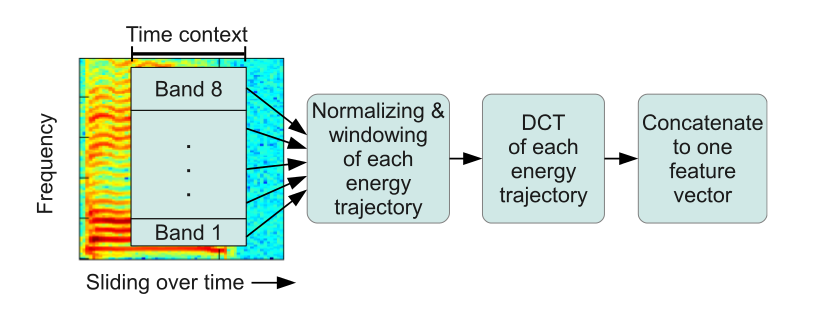
\includegraphics[width=\columnwidth]{images/trap_extraction.png}}}
 \caption{TRAP extraction process \cite{jens}}
 \label{fig:traps}
\end{figure}


\section{Distance calculation}
\subsection{Dynamic Time Warping}
Dynamic Time Warping (DTW) is an algorithm for finding an optimal alignment between two time sequences of vectors $X$ and $Y$, which was originally developed for aligning speech sequences to each other \cite{rabiner}. $X$ and $Y$ are not required to have the same length (i.e. $X = (x_1,...,x_M$) and $Y = (y_1,...,y_N) $). To this end, varying durations of parts of each sequence are allowed. The result is a warping path $W = w_1,...,w_K$ where each element represents an alignment of the elements of the two sequences (i.e. $w_k = (m_k,n_k)$ represents the alignment of the elements $x_{m_k}$ and $y_{n_k}$ of $X$ and $Y$).\\
In classical DTW, the warping path must fulfill three restrictions:
\begin{description}
	\item[1. Boundary condition] The warping path must align the whole sequences to each other - i.e. $w_1 = (1,1)$ and $w_K = (M,N)$.
	\item[2. Step size condition] The warping path may only step sequentially forward in either direction - i.e. $w_{k+1} - w_k \in \{(0,1),(1,0),(1,1)\}$. 
	\item[3. Monotonicity condition] The warping path cannot skip backwards - i.e. $m_1 \leq m_2 \leq ... \leq m_K$ and $n_1 \leq n_2 \leq ... \leq n_K$. (This is, in fact, already implied by condition 2).
\end{description}
A graphic example of such an alignment is given in figure \ref{fig:dtw_example}.\\

\begin{figure}
	\begin{center}
		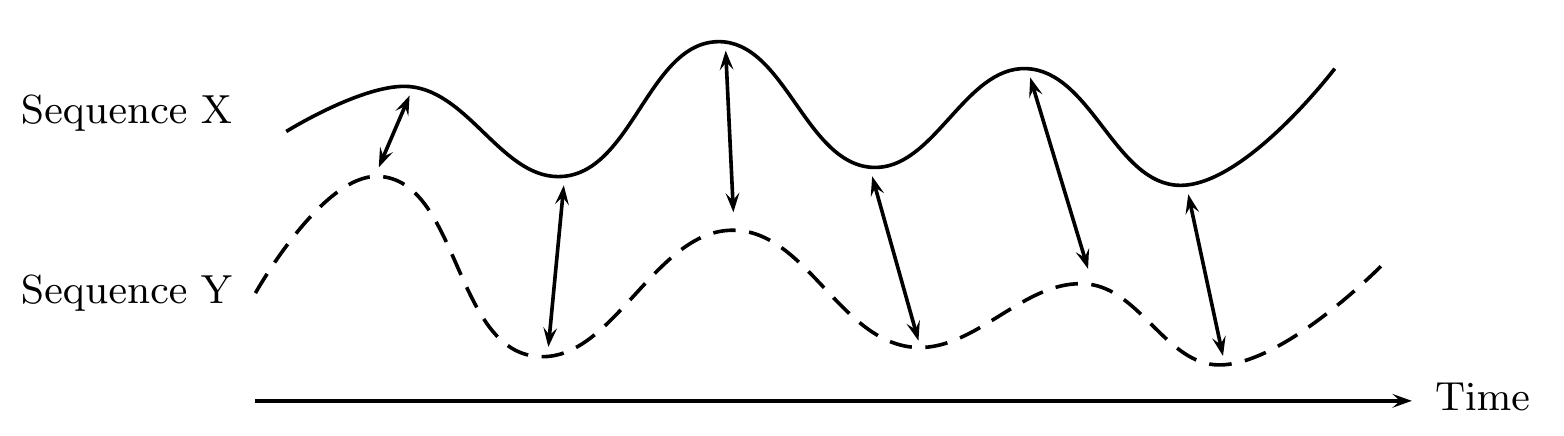
\includegraphics[width=0.8\textwidth]{images/dtw_example.png}
		\caption{Example of a DTW alignment. Alignment between points is represented by the arrows. \cite{meinard_retrieval}}
		\label{fig:dtw_example}
	\end{center}
\end{figure}

A DTW consists of two steps: Cost calculation and path detection. In the cost calculation steps, a local cost $c$ is calculated for all pairs $(x_m, y_n)$, resulting in a cost matrix $C$. An example is shown in figure \ref{fig:dtw_cost}. Common cost functions include the Manhattan distance and the cosine distance (i.e. the complement of the normalized inner product), which was used in this work:
\begin{equation}
c(x_m,y_n) =  1 - cos(\theta)
\end{equation}
where $\theta$ is the angle between $x_m$ and $y_n$.\\

In the second step, an optimal warping path is calculated on the cost matrix. The cost of a warping path is
\begin{equation}
c_W(X,Y) =  \sum_{k=1}^{K} c(x_{m_k}, y_{n_k})
\end{equation}
and the optimal warping path is the one with minimal cost - i.e. the DTW cost:
\begin{equation}
DTW(X,Y) =  \min\{c_W(X,Y)|W \text{ is a warping path}\}
\end{equation}

Consequently, the DTW cost can also be used to compare the quality of alignments of one query sequence to multiple other sequences when taking the varying lengths into account.
%TODO: hier beschreiben?
The path calculation is commonly solved using a Dynamic Programming algorithm \cite{meinard_retrieval}. In this work, the implementation from \cite{ellis_dtw} is used.
\begin{figure}
	\begin{center}
		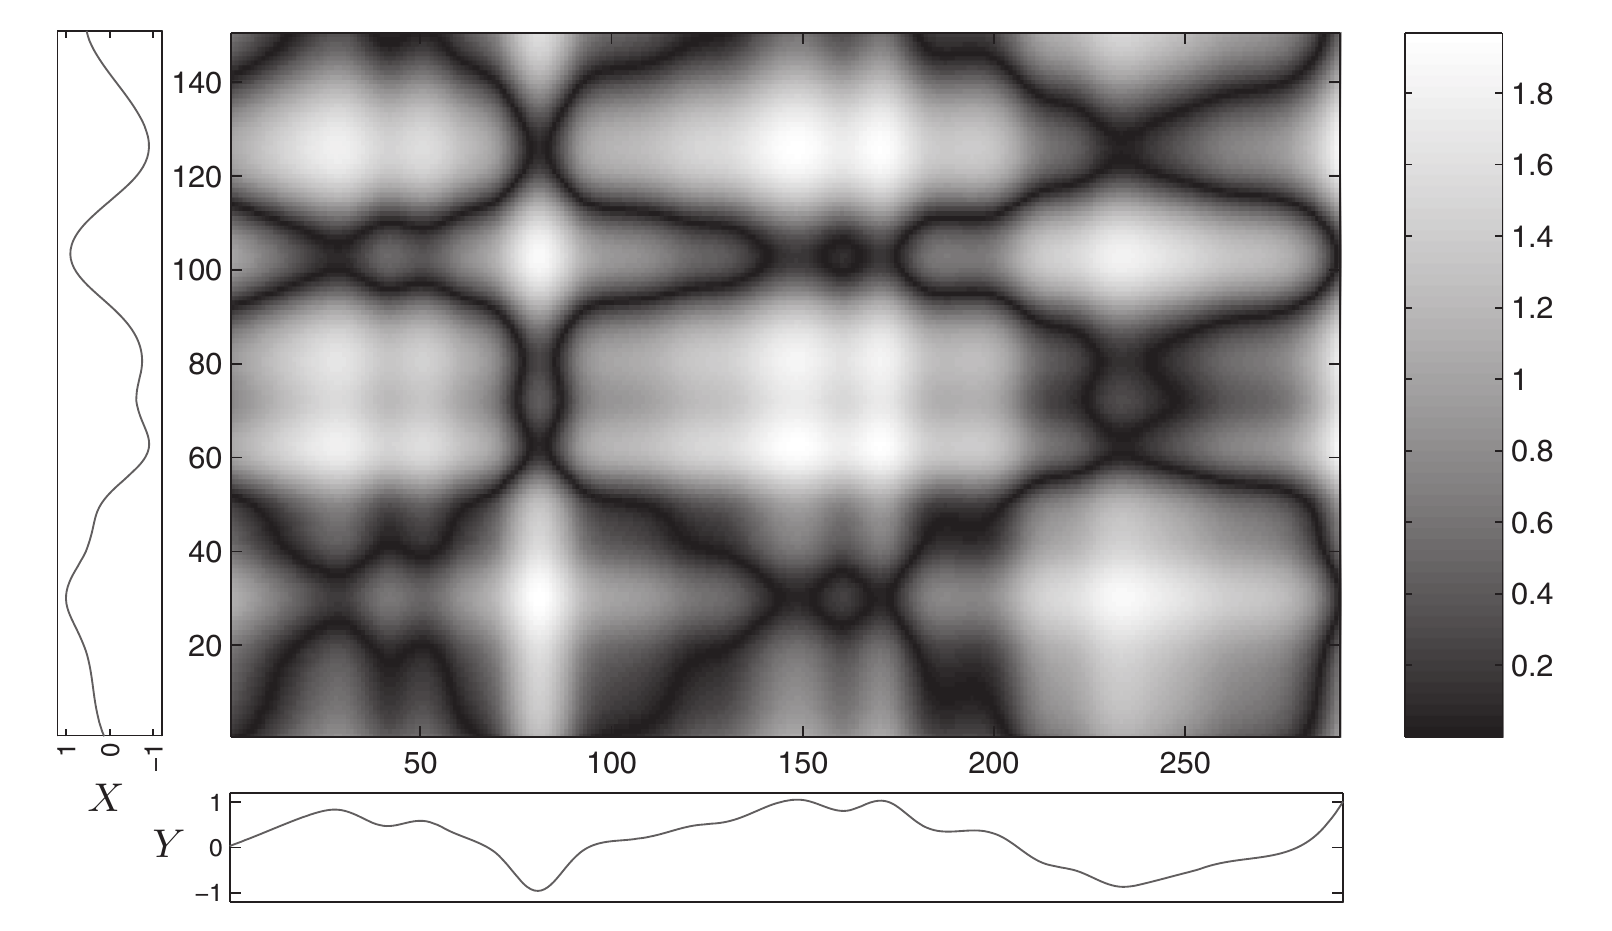
\includegraphics[width=0.8\textwidth]{images/dtw_cost.png}
		\caption{Example of a matrix of costs between two sequences $X$ and $Y$ using the Manhattan distance as the local cost measure. \cite{meinard_retrieval}}
			\label{fig:dtw_cost}
		\end{center}
	\end{figure}


\subsection{Levenshtein Distance}

\section{Machine learning algorithms}
This section describes the various Machine Learning algorithms employed throughout this thesis. Gaussian Mixture Models (GMMs), Hidden Markov Models (HMMs), and Support Vector Machines (SVMs) are three traditional approaches that are used as the basis of many new approaches, and were used for several starting experiments. i-Vector processing is a relatively new, more sophisticated approach that bundles several other machine learning techniques.\\
In recent years, Deep Learning has become the standard for machine learning applications \cite{}. This chapter also describes a new approach that was used extensively in this work: Deep Neural Networks (DNNs).



\subsection{Gaussian Mixture Models}
%256
%!
\subsection{Hidden Markov Models}
%!

\subsection{Support Vector Machines}
%! clean up
In all supervised classification tasks, a training data set and a classification data set are provided. Each of these sets consists of previously extracted features of the training entities (or musical pieces in the case of genre classification) and, for the training data set, annotation labels (or genres in the case of genre classification). The training data set is denoted here as pairs of $\left(\mathbf{x}_{i}, y_{i}\right), i=1..l$, with $\textbf{x}_i \in \mathbb{R}^{n}$ being the feature vectors and $y_{i}$ being their assigned classes. The classifier tries to find similarities behind the training data for each label and separation conditions between the labels. With this information, the classifier is then able to assign a label to the classification data entities.\\
SVMs attempt to solve this problem by grouping the training data vectors $\mathbf{x}_{i}$ and finding separating (hyper-)planes (with the normal vector $\mathbf{w}$ and the offset $b$) between the points of the different classes (or annotation labels) $y_{i}$. In doing so, they try to maximise the margin between the plane and the data points. Additionally, the feature vectors may be transformed into a higher-dimensional space by the function $\phi(\textbf{x}_i)$ to make them more easily separable (as demonstrated in figure \ref{fig:svm_transformation}).\newpage
In \cite{techreport:practical_svm}, this training process is expressed (for a two-class problem) as:
\begin{equation*}
\begin{aligned}
& \min\limits_{\mathbf{w},b,\xi} & & \frac{1}{2}\mathbf{w}^{T}\mathbf{w} + C \sum\limits_{i=1}^{l}\xi_{i} \\
& \text{subject to} & & y_{i}(\mathbf{w}^{T} \phi(\mathbf{x}_{i})+b) \geq 1-\xi_{i} , \\
&&& \xi_{i} \geq 0
\end{aligned}
\end{equation*}
(with $\xi_{i}$ being a slack variable and $C > 0$ being a penalty parameter for the error term, higher $C$s allowing for fewer outliers (\cite{article:intro_svm}).
\begin{figure}[htbp]
	\centering
	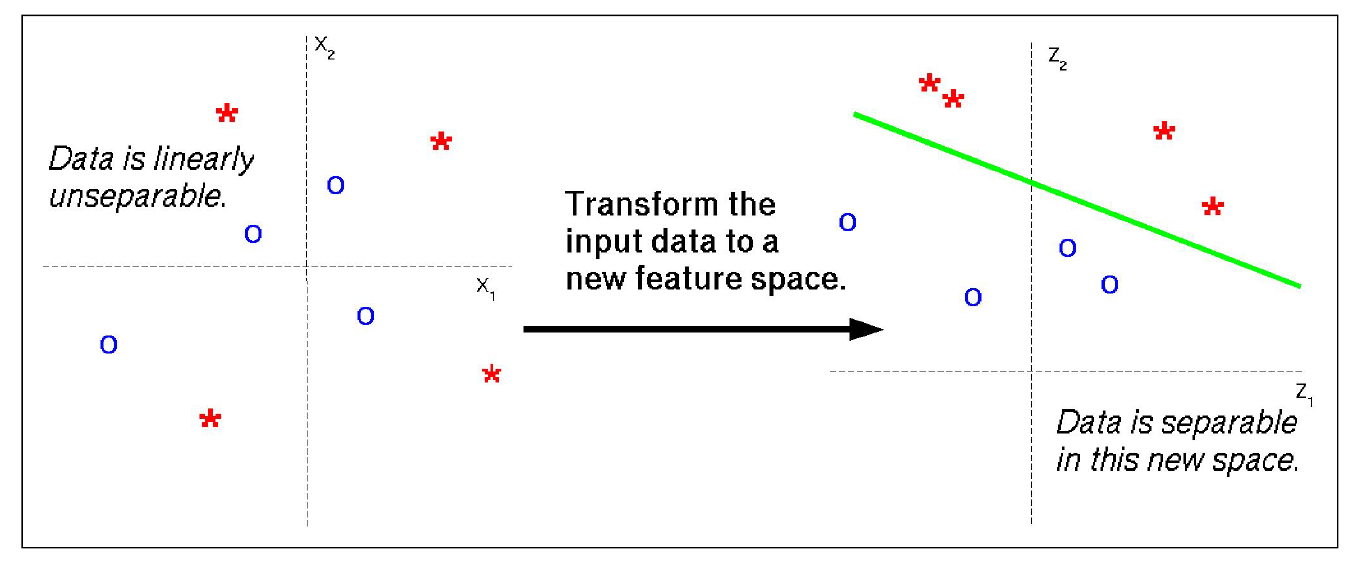
\includegraphics[width=0.9\textwidth]{images/svm_transformation.png}
	\caption{A set of data points which cannot be separated linearly in their original form (left), but can be separated after transformation into another space (right) \cite{article:intro_svm}}
	\label{fig:svm_transformation}
\end{figure}
\medskip
\\
$K(\mathbf{x}_{i},\mathbf{x}_{j}) \equiv \phi(\mathbf{x}_{i})^{T} \phi(\mathbf{x}_{j})$ is called the \textit{kernel function}. Several variants are possible, e.g. a linear one:
\begin{equation}
K(\mathbf{x}_{i},\mathbf{x}_{j}) = \mathbf{x}_{i}^{T}\mathbf{x}_{j}
\end{equation}
It is often useful to use a non-linear kernel because the data points may not be linearly separable (even after the transformation into a higher-dimensional space). An example is shown in figure \ref{fig:svm_kernels}. The RBF kernel (Radial Basis Function) is a popular one:
\begin{equation}
K(\mathbf{x}_{i},\mathbf{x}_{j}) = e^{-\gamma \parallel \mathbf{x}_{i} - \mathbf{x}_{j} \parallel^{2}}, \gamma > 0
\end{equation}
\begin{figure}[htbp]
	\centering
	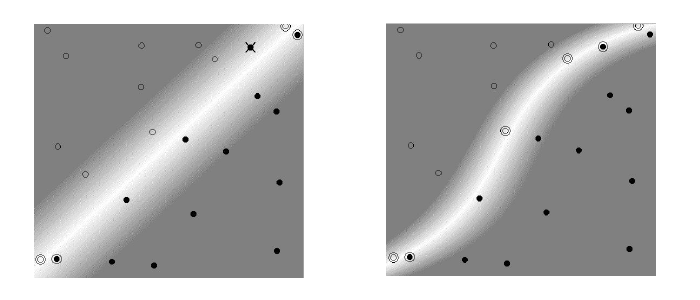
\includegraphics[width=0.9\textwidth]{images/svm_kernels.png}
	\caption{A set of data points which cannot be separated using a linear kernel (left), but can be separated with a polynomial kernel (right) \cite{article:svm_tutorial}}
	\label{fig:svm_kernels}
\end{figure}
\medskip
\\
As can be seen from the above equations, $C$ and $\gamma$ are free parameters. Their optimum values depend on the actual training data vectors. In \cite{techreport:practical_svm}, a grid search during each training is suggested to find them. 
\medskip
\\
The presented training process is appropriate for a two-class problem. For multi-class problems, one-vs-one trainings for all combinations of classes are performed. Then,all of the developed classifiers are used for the classification of the evaluation data and a voting strategy is applied to determine the resulting class. This procedure is not quite in agreement with the one used in the feature selection algorithm (IRMFSP, see section \ref{subsec:irmfsp}), as this algorithm selects features to separate all classes at once, rather than on a one-vs-one basis.


\subsection{i-Vector processing}
I-Vector (identity vector) extraction was first introduced in \cite{Dehak2011} and has since become a state-of-the-art technique for various speech processing tasks, such as speaker verification, speaker recognition, and language identification \cite{Martinez2011}. To our knowledge, it has not been used for any Music Information Retrieval tasks before. \\
The main idea behind i-vectors is that all training utterances contain some common trends, which effectively add irrelevance to the data in respect to training. Using i-vector extraction, this irrelevance can be filtered out, while only the unique parts of the data relevant to the task at hand remain. The dimensionality of the training data is massively reduced, which also makes the training less computationally expensive. As a side effect, all feature matrices are transformed to i-vectors of equal length, eliminating problems that are caused by varying utterance lengths.\\
Mathematically, this assumption can be expressed as:
\begin{equation}
M(u) = m+Tw
\end{equation}
In this equation, $M(u)$ is the GMM supervector for utterance $u$. The supervector approach was first presented in \cite{reynolds00} and has since been successfully applied to a number of speech recognition problems. A music example can be found in \cite{Charbuillet2011}. $m$ represents the language- and channel-independent component of $u$ and is estimated using a Universal Background Model (UBM). $T$ is a low-rank matrix modeling the relevant language- and channel-related variability, the so-called Total Variability Matrix. Finally, $w$ is a normally distributed latent variable vector: The i-vector for utterance $u$.

\paragraph*{Step 1: UBM training} A Universal Background Model (UBM) is trained using Gaussian Mixture Models (GMMs) from all utterances. This UBM models the characteristics that are common to all of them.
\paragraph*{Step 2: Statistics extraction} 0th and 1st order Baum-Welch statistics are calculated for each of the utterances from the UBM according to:
\begin{equation}
N_c(u)=\sum_{t=1}^{L} P(c|y_t,\Omega)
\end{equation}
\begin{equation}
\widetilde{F_c}(u)=\sum_{t=1}^{L} P(c|y_t,\Omega)(y_t-m_c)
\end{equation}
where $u={y_1,y_2,...,y_L}$ denotes an utterance with $L$ frames, $c=1,...,C$ denotes the index of the Gaussian component, $\Omega$ denotes the UBM,  $m_c$ is the mean of the UBM mixture component $c$, and $P(c|y_t,\Omega)$ denotes the posterior probability that the frame $y_t$ was generated by mixture component $c$. As the equation shows, the 1st order statistics are centered around the mean of each mixture component.\\
\paragraph*{Step 3: T matrix training}
Using the Baum-Welch statistics for all utterances, the Total Variability Matrix $T$ is now trained iteratively according to:
\begin{equation}\label{equ:trainT}
w = (I+T^t \Sigma^{-1} N (u) T)^{-1}T^t \Sigma^{-1} \widetilde{F}(u)
\end{equation}
using Expectation Maximization.
\paragraph*{Step 4: Actual i-vector extraction}
Finally, an i-vector $w$ can be extracted for each utterance using equation \ref{equ:trainT} again. This can also be done for unseen utterances, using a previously trained $T$.


\subsection{Artificial Neural Networks}
%!

\section{Evaluation}
\subsection{Evaluation of phoneme recognition and alignment tasks}
%alignment? - duration acc. - no, mean error
\subsection{Evaluation of language identification tasks}
\subsection{Evaluation of keyword spotting tasks}

\section{Speech recognition systems}
\subsection{Phoneme recognition}
\subsection{Forced alignment}
\subsection{Language identification}
Language identification has been extensively researched in the field of Automatic Speech Recognition since the 1980's. A number of successful algorithms have been developed over the years. An overview over the fundamental techniques is given by Zissman in \cite{zissman}.\\
Fundamentally, four properties of languages can be used to discriminate between them:
\begin{description}
	\item[Phonetics] The unique sounds that are used in a given language.
	\item[Phonotactics] The probabilities of certain phonemes and phoneme sequences.
	\item[Prosody] The ``melody'' of the spoken language.
	\item[Vocabulary] The possible words made up by the phonemes and the probabilities of certain combinations of words.
\end{description}
Even modern system mostly focus on phonetics and phonotactics as the distinguishing factors between languages. Vocabulary is sometimes exploited in the shape of language models.\\
Zissman mentions Parallel Phone Recognition followed by Language Modeling (PPRLM) as one of the basic techniques. It requires audio data, language annotations, and phoneme annotations for each utterance. In order to make use of vocabulary characteristics, full sentence annotations and word-to-phoneme dictionaries are also necessary.\\
Using the audio and phoneme data, acoustic models are trained. They describe the probabilities of certain sound and sound sequences occurring. This is done separately for each considered language. Similarly, language models are generated using the sentence annotations and the dictionary. These models describe the probabilities of certain words and phrases. Again, this is done for each language.\\
New audio examples are then run through all pairs of acoustic and language models, and the likelihoods produced by each model are retained. The highest acoustic likelihood, the highest language likelihood, or the highest combined likelihood are then considered to determine the language. This approach achieves up to $79\%$ accuracy for ten languages \cite{muthusamy}.\\
Another approach uses the idea to train Gaussian Mixture Models for each language. This technique can be considered a ``bag of frames'' approach, i.e. the single data frames are considered to be statistically independent of each other. The generated GMMs then describe probability densities for certain characteristics of each language. Using these, the language of new audio examples can be easily determined.\\
GMM approaches used to perform worse than their PPRLM counterparts, but the development of new features has made the difference negligible \cite{singer}. They are in general easier to implement since only audio examples and their language annotations are required. Allen et al. \cite{allen} report results of up to $76.4\%$ accuracy for ten languages. Different backend classifiers, such as Multi-Layer Perceptrons (MLPs) and Support Vector Machines (SVMs) \cite{campbell} have also been used successfully instead of GMMs.

\subsection{Keyword spotting}






%ozeki??

\chapter{State of the Art}	\label{chap:sota}
This chapter presents an overview over the various published approaches for the tasks considered in this work. One key issue is comparability: As in many MIR tasks, data sets are not publicly available and vary widely, which makes  comparison of the individual approaches very difficult. As the following sections show, there is also disagreement about evaluation measures in all of these tasks.\\

For these reasons, new, reproducible data sets were created for this work (presented in the next chapter). As described in the individual chapters, the most frequently used measures were employed for evaluation.

\section{From speech to singing} \label{sec:sota_speechtosinging}
Singing presents a number of challenges for speech recognition when compared to pure speech \cite{loscos}\cite{goto_alignment}\cite{kruspe_kws1}. The following factors make speech recognition on singing more difficult than on speech, and necessitate the adaption of existing algorithms.
\begin{description}
 \item[Larger pitch fluctuations] A singing voice varies its pitch to a much higher degree than a speaking voice. It often also has very different spectral properties.
 \item[Larger changes in loudness] In addition to pitch, loudness also fluctuates much more in singing than in speech.
 \item[Higher pronunciation variation] The musical context causes singers to pronounce certain sounds and words differently than if they were speaking them.
 \item[Larger time variations] In singing, sounds are often prolonged for a certain amount of time to fit them to the music. Conversely, they can also be shortened or left out completely.
 In order to research this effect more closely, a small experiment was performed on a speech corpus and on a singing data set (\textit{TIMIT} and \textit{ACAP}, see chapter \ref{chap:datasets}): The standard deviations for all the phonemes in each data set were calculated. The result is shown in figure \ref{fig:phoneme_stats}, confirming that the variation in singing is much higher. This is particularly pronounced for vowels.
 \item[Different vocabulary] In musical lyrics, words and phrases often differ from normal conversational script. Certain words and phrases have different probabilities of occurring in speech versus singing (e.g. a higher focus on emotional topics in singing).
 \item[Background music] This is the biggest interfering factor with polyphonic recordings. Harmonic and percussive instruments add a big amount of spectral components to the signal, which lead to confusion in speech recognition algorithms. Ideally, these components should be removed or suppressed in a precursory step. This could be achieved, for example, by employing source separation algorithms, but such algorithms add additional artifacts to the signal, and may not even be sufficient for this purpose at the current state of research.
 Vocal Activity Detection (VAD) could be used as a non-invasive first step in order to discard segments of songs that do not contain singing voices. However, such algorithms often make mistakes in the same cases that are problematic for speech recognition algorithms (e.g. instrumental solos \cite{schlueter2016_ismir}).
 For these reasons, most of the experiments in this work were performed on unaccompanied singing. The integration of the mentioned pre-processing algorithms would be a very interesting next step of research.
The lyrics-to-singing alignment algorithms presented in chapter \ref{chap:retrieval_alignment} are an exception. Those were also tested on polyphonic music, and the algorithms appear to be largely robust to these influences.
 \end{description}
 
 %Mehr Beispiele aus Goto-Kapitel
 %Sundberg!
 % Vowels vs. Consonants (1. Mesaros-Paper + recognition of phonemes and words...)

\begin{figure*}
	\begin{center}
		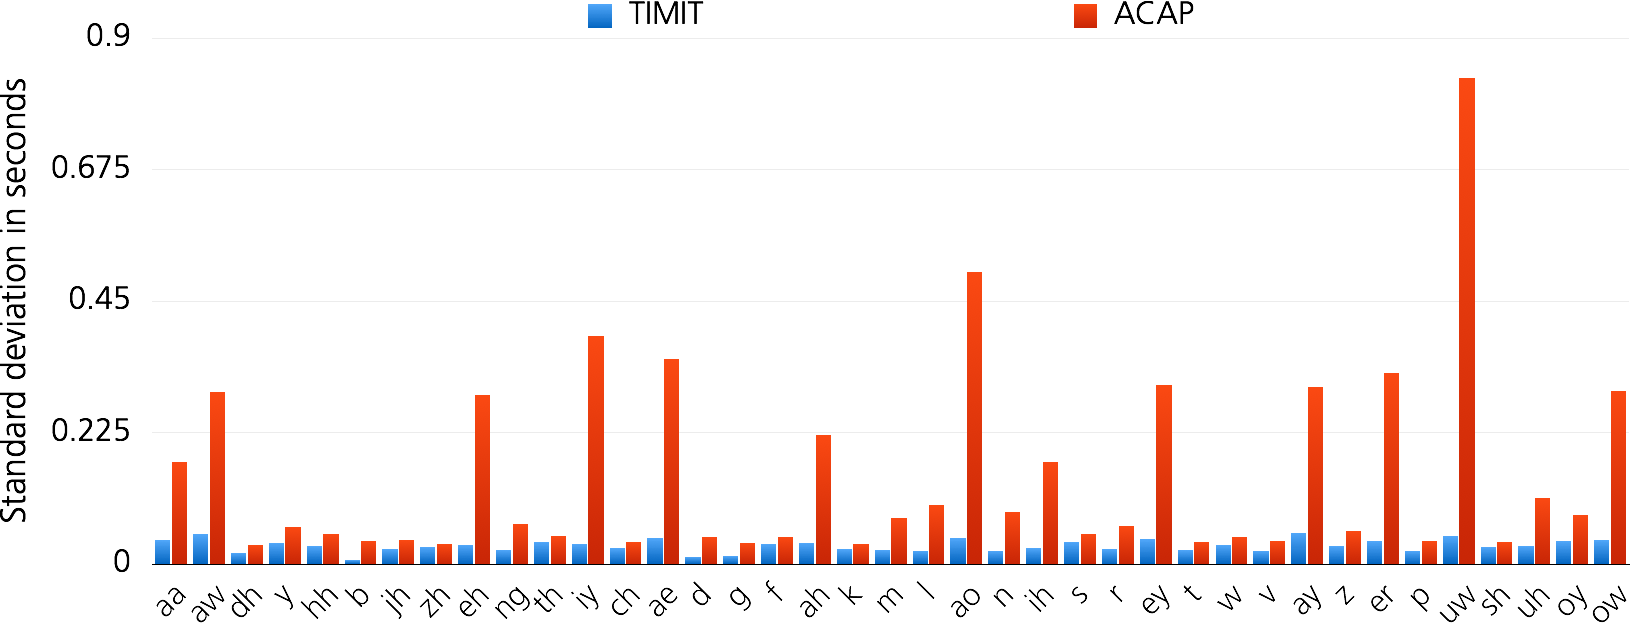
\includegraphics[width=1\textwidth]{images/phoneme_stats.png}
		\caption{Standard deviations of phoneme durations in the \textit{TIMIT} and \textit{ACAP} data sets.}
		\label{fig:phoneme_stats}
	\end{center}
\end{figure*}

The broad field of analyzing various aspects of the singing voice was summed up as \textit{singing information processing} in \cite{singing_information_processing} (updated in \cite{singing_information_processing2}). A first collection of singing voice recordings for Music Information Retrieval was created in 2005 \cite{jap_humming} (this database is not used in this work because it is not publicly available).

%describe tasks here??

\section{Phoneme recognition} \label{sec:sota_phonerec}
%\subsection{Phoneme recognition in speech}
%\subsection{Phoneme recognition in singing}
Due to the factors mentioned above in section \ref{sec:sota_speechtosinging}, phoneme recognition on singing is more difficult than on clean speech. It has only been a topic of research for a few years, and there are few publications.\\

One of the earliest systems was presented by Wang et al. in 2003 \cite{WangLC03}. Acoustic modeling is performed with triphone HMMs trained on read speech in Taiwanese and Mandarin. The language model is completely restricted to lines of lyrics in the test dataset. Testing is performed on 925 unaccompanied sung phrases in these language. Due to the highly specific language model, the Word Error Rate is just $0.07$.\\

Hosoya et al. employ a similarly classic approach from ASR that employs monophone HMMs also trained on read speech for acoustic modeling \cite{Hosoya2005} (2005). These models are adapted to singing voices using the Maximum Likelihood Linear Regression (MLLR) technique \cite{mllr}. Language modeling is performed with a Finite State Automaton (FSA) specific to the Japanese language, making it more flexible than the previous system.
The system is tested on five-word unaccompanied phrases, while the adaptation is performed on 127 choruses performed by different singers. The Word Error Rate is $0.36$ without the adaptation, and $0.27$ after adaptation.\\

In 2007, Gruhne et al. presented a classic approach that employs feature extraction and various machine learning algorithms to classify singing into 15 phoneme classes \cite{Gruhne2007}\cite{Gruhne2007a}. The specialty of this approach lies in the pre-processing: At first, fundamental frequency estimation is performed on the audio input, using a Multi-Resolution Fast Fourier Transform (MRFFT) \cite{inproceedings:dressler}. Based on the estimated fundamental frequency, the harmonic partials are retrieved from the spectrogram. Then, a sinusoidal re-synthesis is carried out, using only the detected fundamental frequency and partials. Feature extraction is then performed on this re-synthesis instead of the original audio. Extracted features include MFCCs, PLPs, Linear Predictive Coding features (LPCs), and Warped Linear Predictive Coding features (WLPCs \cite{lpc}). MLP, GMM, and SVM models are trained on the resulting feature vectors. The re-synthesis idea comes from a singer identification approach by Fujihara \cite{fujihara_identification}. The approach is tested on more than 2000 separate, manually annotated phoneme instances from polyphonic recordings. Only one feature vector per phoneme instance is calculated. Using SVM models, $56\%$ of the tested instances were classified correctly into one of the 15 classes. This is considerably better than the best result without the re-synthesis step ($34\%$). In \cite{szepannek} (2010), the approach is expanded by testing a larger set of perceptually motivated features, and more classifiers. No significant improvements are found when using more intricate features, and the best-performing classifier remains an SVM.\\

Fujihara et al. described an approach based on spectral analysis in 2009 \cite{fujihara_phonemes}. The underlying idea is that spectra of polyphonic music can be viewed as the weighted sum of two types of spectra: One for the singing voice, and one for the background music. This approach then models these two spectra as probabilistic spectral templates. The singing voice is modeled by multiplying a vocal envelope template, which represents the spectral structure of the singing voice, with a harmonic filter, which represents the harmonic structure of the produced sound itself. This is analogous to the source-filter model of speech production \cite{Fant1981}. For recognizing vowels, five such harmonic filters are prepared (\texttt{a - e - i - o - u}). Vocal envelope templates are trained on voice-only recordings, separated by gender. Templates for background music are trained on instrumental tracks. In order to recognize vowels, the probabilities for each of the five harmonic templates are estimated. 
As described, the phoneme models are gender-specific and only model five vowels, but also work for singing with instrumental accompaniment. The approach is tested on 10 Japanese-language songs. The best result is $65\%$ correctly classified frames, compared to the $56\%$ with the previous approach by this team, based on GMMs.\\

%As a side product, the algorithm also estimates the fundamental frequency of the singing voice
In these experiments, the fundamental frequencies $F_0$ (which are necessary for the recognition) are manually provided. The approach is further expanded in \cite{concurrent_f0_phonemes} to be able to detect them concurrently with the phonemes. Additionally, models can directly be trained on polyphonic music rather than monophonic singing voices. The over-all best results degrade by around 4 percent points, but this method is much more flexible.\\

In 2009, Mesaros et al. picked Hosoya's approach back up by using MFCC features and GMM-HMMs for acoustic modeling \cite{Mesaros2009} and adapting the models for singing voices. These models are trained on the CMU ARCTIC speech corpus\footnote{\url{http://festvox.org/cmu_arctic/}}. Then, different MLLR techniques for adapting the models to singing voices are tested \cite{mllr}.
The adaptation and test corpus consists of 49 voice-only fragments from 12 pop songs with durations between 20 and 30 seconds. The best results are achieved when both the means and variances of the Gaussians are transformed with MLLR. The results improved slightly when not just a single transform was used for all phonemes, but when they were grouped into base classes beforehand, each receiving individual transformation parameters. The best result is around $0.79$ Phoneme Error Rate on the test set.\\

In \cite{Mesaros2010} and \cite{Mesaros2011}, language modeling is added to the presented approach. Phoneme-level language models are trained on the CMU ARCTIC corpus as unigrams, bigrams, and trigrams, while word-level bigram and trigram models are trained on actual song lyrics in order to match the application case. The output from the acoustic models is then refined using these language models. The approach is tested on the clean singing corpus mentioned above and on 100 manually selected fragments of 17 polyphonic pop songs. To facilitate recognition on polyphonic music, a vocal separation algorithm is introduced \cite{virtanen_separation}.
Using phoneme-level language modeling, the Phoneme Error Rate on clean singing is reduced to $0.7$. On polyphonic music, it is $0.81$. For the word recognition approach, the Word Error Rate is $0.88$ on clean singing and $0.94$ on the polyphonic tracks.\\

A more detailed voice adaptation strategy is tested in \cite{mesaros2}. Instead of adapting the acoustic models with mixed-gender singing data, they are adapted gender-wise, or to specific singers. With the gender-specific adaptations, the average Phoneme Error Rate on clean singing is lowered to $0.81$ without language modeling and $0.67$ with language modeling. Singer-specific adaptation does not improve the results, probably because of the very small amount of adaptation data in this case.\\
%mvcivar, hosoya

In \cite{McVicar2014} (2014), McVicar et al. build on a very similar baseline system, but also exploit repetitions of choruses to improve transcription accuracy. This has been done for other MIR tasks, such as chord recognition, beat tracking, and source separation. They propose three different strategies for combining individual results: Feature averaging, selection of the chorus instance with the highest likelihood, and combination using the Recogniser Output Voting Error Reduction (ROVER) algorithm \cite{rover}. They also employ three different language models, two of which were matched to the test songs (and therefore not representative for general application). 20 unaccompanied, English-language songs from the RWC database \cite{rwc} were used for testing; chorus sections were selected manually. The best-instance selection and the ROVER strategies improve results considerably; with the ROVER approach and a general-purpose language model, the Phoneme Error Rate is at $0.74$ (versus $0.76$ in the baseline experiment), while the Word Error Rate is improved from $0.97$ to $0.9$. Interestingly, cases with a low baseline result benefit the most from exploiting repetition information.\\

The final system was proposed by Hansen in 2012 \cite{jens}. It also employs a classic approach consisting of a feature extraction step and a model training step. Extracted features are MFCCs and TRAP features. Then, MLPs are trained separately on both feature sets. As mentioned in section \ref{subsec:tech_trap}, each feature models different properties of the considered phonemes: Short-term MFCCs are good at modeling the pitch-independent properties of stationary sounds, such as sonorants and fricatives. On the flip side, TRAP features are able to model temporal developments in the spectrum, forming better representations for sounds like plosives or affricates.
The results of both MLP classifiers are combined via a fusion classifier, also an MLP. Then, Viterbi decoding is performed on its output.
The approach is trained and tested on a data set of 13 vocal tracks of pop songs, which were manually annotated with a set of 27 phonemes. The combined system achieves a recall of $0.48$, compared to $0.45$ and $0.42$ for the individual MFCC and TRAP classifiers respectively. This confirms the assumption that the two features complement each other. The phoneme-wise results further corroborate this.\\

Various publications suggest that phoneme recognition is not a trivial task for human listeners either. Recognition rates are in the range of 70 to 90\% for native speakers, depending on factors such the signal quality and the type of phoneme \cite{weber_smits}\cite{meyer_waechter}. For singing, much lower rates are reported \cite{hollien}.


\section{Language identification}
A first approach for language identification in singing was proposed by Tsai and Wang in 2004 \cite{tsai_wang}. At its core, the algorithm is similar to Parallel Phone Recognition followed by Language Modeling (PPRLM). However, instead of full phoneme modeling, they employ an unsupervised clustering algorithm to the input feature data and tokenize the results to form language-specific codebooks (plus one for background music). Following this, the results from each codebook are run through matching language models to determine the likelihood that the segment was performed in this language. Prior to the whole process, Vocal Activity Detection is performed. This is done by training GMMs on segments of each language and on non-vocal segments. MFCCs are used as features.
The approach is tested on 112 English- and Mandarin-language polyphonic songs each, with 32 of them being the same songs performed in both languages. A classification accuracy of $0.8$ is achieved on the non-overlapping songs. On the overlapping songs, the accuracy is only $0.7$, suggesting some influence of the musical material (as opposed to the actual language characteristics). Misclassifications occur more frequently on the English-language songs, possibly because of accents of Chinese singers performing in English and because of louder background music.\\

A second, simpler approach was presented by Schwenninger et al. in 2006 \cite{schwenninger}. They also extract MFCC features and then use these to directly train statistical models for each language. Three different pre-processing strategies are tested: Vocal Activity Detection, distortion reduction, and azimuth discrimination. Vocal Activity Detection (or vocal/non-vocal segmentation) is performed by thresholding the energy in high-frequency bands as an indicator for voice presence over 1-second windows. This leaves a relatively small amount of material per song. Distortion reduction is employed to discard strong drum and bass frames where the vocal spectrum is masked by using a Mel-scale approach. Finally, azimuth discrimination attempts to detect and isolate singing voices panned to the center of the stereo scene.
The approach is tested on three small data sets of speech, unaccompanied singing, and polyphonic music. Without pre-processing steps, the accuracies are $0.84$, $0.68$, and $0.64$ respectively, highlighting the increased difficulty of language identification on singing versus speech, and on polyphonic music versus pure vocals. On the polyphonic corpus, the pre-processing steps do not improve the result.\\

In 2011, Mehrabani and Hansen presented a full PPRLM approach for sung language identification. MFCC features are run through phoneme recognizers for Hindi, German, and Mandarin; then, the results are scored by individual language models for each considered language. In addition, a second system is employed which uses prosodic instead of phonetic tokenization. This is done by modeling pitch contours with Legendre polynomials and then quantizing these vectors with previously trained GMMs. The results are then again used as inputs to language models.
The approach is trained and tested on a corpus containing 12 hours of unaccompanied singing and speech in Mandarin, Hindi, and Farsi. The average accuracies for singing are $0.78$ and $0.43$ for the phoneme- and prosody-based systems respectively, and $0.83$ for a combination of both.\\

Also in 2011, Chandrasekhar et al. presented a very interesting approach for language identification on music videos, analyzing both audio and video features \cite {chandrasekhar}. On the audio side, the spectrogram, volume, MFCCs, and perceptually motivated Stabilized Auditory Images (SAI) are used as inputs. One-vs-all SVMs are trained for each language. The approach is trained and tested on 25,000 music videos in 25 languages. Using audio features only, the accuracy is $0.45$; combined with video features, it rises to $0.48$. It is interesting to note that European languages achieve much lower accuracies than Asian and Arabic ones. English, French, German, Spanish and Italian rank below $0.4$, while languages like Nepali, Arabic, and Pashto achieve accuracies above $0.6$. It is possible that the language characteristics of European languages make them harder to discriminate (especially against each other) than others.

\section{Keyword spotting}
%\subsection{Keyword spotting in speech}
%Igor Sz? oke, Petr Schwarz, Pavel Matejka, Luk?as Bur-get, Martin Karafi? at, Michal Fapso, and Jan Cernock`y.Comparison of keyword spotting approaches for infor- mal continuous speech. In Interspeech, pages 633?636, 2005.
%\subsection{Keyword spotting in singing}
%SPEECH HERE
%pedro!!
Keyword spotting in singing was first attempted in 2008 by Fujihara et al. \cite{hyperlinking_lyrics}. Their method starts with a phoneme recognition step, which is once again based on the vocal re-synthesis method described in \cite{fujihara_identification}. MFCCs and power features are extracted from the re-synthesized singing and used as inputs to a phoneme model, similar to Gruhne's phoneme recognition approach mentioned above in section \ref{sec:sota_phonerec}.  Three phoneme models are compared: One trained on pure speech and adapted with a small set of singing recordings, one adapted with all recordings, and one trained directly on singing. Viterbi decoding is then performed using keyword-filler HMMs to detect candidate segments where keywords may occur. These segments are then re-scored through the filler HMM to verify the occurrence. When the textual lyrics for a song are known, the system offers the additional possibility to use lyrics-to-audio alignment instead.
The method is tested on 79 unaccompanied Japanese-language songs from the RWC database \cite{rwc} with keywords containing at least 10 phonemes. The Phoneme Error Rate is $0.73$ for the acoustic models trained on speech, $0.67$ for the adapted models, and $0.49$ for the models trained on singing (it should be mentioned that the same songs were used for training and testing, although a cross-validation experiment shows that the effect is negligible). The employed evaluation measure is ``link success rate'', describing the percentage of detected phrases that were linked correctly to other occurrences of the phrase in the data set. In that sense, it is a sort of accuracy measure. The link success rate for detecting the keywords is $0.3$. The authors show that the result depends highly on the number of phonemes in the considered keyword, with longer keywords being easier to detect.\\

Building on this approach, a system named ``LyricListPlayer'' was developed by Nakano and Goto in 2016 \cite{lyriclistplayer}. In this case, however, keywords are exclusively detected using lyrics-to-audio alignment and a subsequent search on the textual lyrics (which need to be available in advance). Monophone HMM acoustic models for English and Japanese similar to the ones mentioned above are employed. Those models are trained on a relatively small number of songs from the RWC database \cite{rwc} using power-based and MFCC features. An interesting addition is the further processing of these alignments: Natural Language Processing (NLP) techniques for topic modeling are applied to the lyrics, allowing users to search for similar keywords or phrases.\\

In 2012, Mercado et al. presented an approach to keyword spotting in singing based on a different principle: DTW between a sung query and the requested phrase in the song recording. In particular, Statistical Sub-Sequence DTW is the algorithm employed for this purpose. MFCCs are used as feature inputs on which the costs of the warping paths are calculated from all possible starting points to obtain candidate segments, which are then further refined to find the most likely position.
The approach is tested on a set of vocal tracks of 19 pop songs (see section \ref{subsec:data_hansen}) as the references, and recordings of phrases sung by amateur singers as the queries, but no quantitative results are given. The disadvantage of this approach lies in the necessity for audio recordings of the key phrases, which need to have at least similar timing and pitch as the reference phrases.\\

Finally, Dzhambazov et al. developed a score-aided approach to keyword spotting in 2015 \cite{dzhambazov_ismir}. A user needs to select a keyword phrase and a single recording in which this phrase occurs. The keyword is then modeled acoustically by concatenating recordings of the constituent phonemes (so-called acoustic keyword spotting). Similar to Mercado's approach, Sub-Sequence DTW is performed between the acoustic template and all starting positions in the reference recording to obtain candidate segments. These segments are then refined by aligning the phonemes to the score in these positions to model their durations. This is implemented with Dynamic Bayesian Network HMMs. Then, Viterbi decoding is performed to re-score the candidate segments and obtain the best match.
The approach is tested on a small set of unaccompanied Turkish-language recordings of traditional Makam music. The Mean Average Precision (MAP) for the best match is $0.08$ for the DTW approach only, and $0.05$ for the combined approach. For the Top-6 results, the MAPs are $0.26$ and $0.38$ respectively.


\section{Lyrics-to-audio alignment}
%\subsection{Forced alignment in speech}
%\subsection{Forced alignment in singing}
%mesaros
%Three techniques for im- proving automatic synchronization between music and lyrics: Fricative detection, filler model, and novel feature vectors for vocal activity detection
In contrast to the other tasks discussed in this chapter, the task of lyrics-to-audio alignment has been the focus of many more publications. A comprehensive overview until 2012 is given in \cite{goto_alignment}.\\

A first approach was presented in 1999 by Loscos et al. \cite{loscos}. The standard forced alignment approach from speech recognition is adapted to singing. MFCCs are extracted first, and then a left-to-right HMM is employed to perform alignment via Viterbi decoding. Some modifications are made to the Viterbi algorithm to allow for low-delay alignment. The approach is trained and tested on a very small (22 minutes) database of unaccompanied singing, but no quantitative results are given.\\

The first attempt to synchronize lyrics to polyphonic recordings was made by Wang et al. in 2004 \cite{Wang2004}. They propose a system, named ``LyricAlly'', to provide line-level alignments for karaoke applications. Their approach is heavily based on musical structure analysis. First, the hierarchical rhythm structure of the song is estimated. The result is combined with an analysis of the chords and then used to split the song into sections by applying a chorus detection algorithm. Second, Vocal Activity Detection (VAD) using HMMs is performed on each section. Then, sections of the text lyrics are assigned to the detected sections (e.g. verses, choruses). In the next step, the algorithm determines whether the individual lines of the lyrics match up with the vocal sections detected by the VAD step. If they do not, grouping or partitioning is performed. This is based on the assumption that lyrics match up to rhythmic bars as determined by the hierarchical rhythm analysis. The expected duration of each section and line is estimated using Gaussian distributions of phoneme durations from a singing data set. In this manner, lines of text are aligned to the detected vocal segments. The approach is tested on 20 manually annotated pop songs. On the line level, the average error is $0.58$ seconds for the starting points and $-0.48$ seconds for the durations. The system components are analyzed in more detail in \cite{lyrically}.\\

In 2006, the same team presented an approach that also performs rhythm and bar analysis to facilitate syllable-level alignment \cite{Iskandar:2006}. For the phoneme recognition step, an acoustic model is trained on speech data and adapted to singing using the previously mentioned 20 songs. The possible syllable positions in the alignment step are constrained to the note segments detected in the rhythm analysis step. Due to annotator disagreement on the syllable level, the evaluation is performed on the word level. On three example songs, the average synchronization error rate is $0.19$ when allowing for a tolerance of 1/4 bar.\\  

Sasou et al. presented a signal parameter estimation method for singing employing an auto-regressive HMM (AR-HMM) in 2005 \cite{Sasou2005AnAN}. This method is particularly suited for modeling high-pitched signals, which is important for singing voices and usually not a focus in speech processing techniques. Models trained on speech are adapted to singing using MLLR. For evaluation, the method is applied to the task of lyrics-to-audio alignment and tested on 12 Japanese-language songs. For each song, a specific language model is prepared. The correct word rate is $0.79$.\\

Chen et al. presented an approach based on MFCC features and Viterbi alignment in 2006 \cite{popular_synchronization}. Vocal Activity Detection is performed as a pre-processing step, and then GMM-HMMs are used for Viterbi alignment between the audio and the lyrics. Once again, MLLR is used to adapt the acoustic models to singing. In addition, the grammar is specifically tailored to the lyrics. On a data set of Chinese songs by three singers, a boundary accuracy of $0.76$ is obtained on the syllable level.\\

A similar approach which does not require in-depth music analysis was presented by Fujihara et al. in 2006 \cite{fujihara_alignment}. Once again, a straightforward Viterbi alignment method from speech recognition is refined by introducing three singing-specific pre-processing steps: Accompaniment sound reduction, Vocal Activity Detection, and phoneme model adaptation.
For accompaniment reduction, the previously mentioned harmonic re-synthesis algorithm from \cite{fujihara_identification} is used. For Vocal Activity Detection, a HMM is trained on a small set of unaccompanied singing using LPC-derived MFCCs and fundamental frequency ($F_0$) differences as features. The HMM can be parameterized to control the rejection rate. For the phoneme model adaptation, three consecutive steps are tested: Adaptation to a clean singing voice, adaptation to a singing voice segregated with the accompaniment reduction method, and on-the-fly adaptation to a specific singer. MFCC features are used for the Viterbi alignment, which is performed on the vowels and syllabic nasals (\texttt{/m/, /n/, /l/}) only.
Ten Japanese pop songs were used for testing. Evaluation was done on the phrase level by calculating the proportion of the duration of correctly aligned sections to the total duration of the song. For eight of the ten songs, this proportion was $0.9$ or higher when using the complete system, which the authors judge as satisfactory. Generally, the results are lower for performances by female singers, possibly because of the higher $F_0$s. These performances also benefit the most from the Vocal Activity Detection step, even though its performance is also somewhat worse for female singing. All three levels of phoneme model adaptations contribute to the success of the approach.\\

In 2008, the authors improved upon this system with three modifications: Fricative detection, filler models, and new features for the Vocal Activity Detection step \cite{fujihara}. Fricative detection is introduced because the previous system was only based on vowels and nasals, due to the fact that the harmonic re-synthesis discards other consonants. In the new system, fricatives are detected before this step and then retained for the alignment (stop phonemes are not used because they are too short).
The filler model is employed because singers sometimes add extraneous lyrics (like ``la la la'' or ``yeah'') to their performances.
As mentioned above, Vocal Activity Detection does not work as well for female performances because of inaccuracies in the spectral envelope estimation in higher-pitched regions. For this reason, the features are replaced in the new version by comparing the power of the harmonic components directly with those of similar $F_0$ regions.
The approach is again evaluated on ten Japanese pop songs. The original system produces an average accuracy of $0.81$, which is raised to $0.85$ with the new improvements.
In \cite{FujiharaGOO11}, the whole system is presented succinctly and evaluated in more detail. Additionally, integration into a music playback interface is described. The system is expanded in \cite{vocarefiner}, where users can select sung phrases and record new versions of them to improve their performances.\\

Mauch et al. augmented the same approach in 2010 by using chord labels, which are often available in combination with the lyrics on the internet \cite{mauch_alignment2010}\cite{mauch_alignment2}. Chords usually have longer durations than individual phonemes, and are therefore easier to detect. In this way, they provide a coarse alignment, which can be used to simplify the shorter-scale phoneme-level alignment. A chroma-based approach is used to estimate the chords. Information about the chord alignments is directly integrated into the HMM used for alignment.
In \cite{mauch_alignment2}, a large range of parameterizations is tested on 20 English-language pop songs. The highest accuracy for the baseline approach (without chord information) is $0.46$. Using chord position information, this rises to $0.88$. Interestingly, Vocal Activity Detection improves the result when not using chords, but decreases it for the version with chord alignments, possibly because the coarse segmentation it provides is already covered by the chord detection in the second case. The method is also able to cope with incomplete chord transcriptions while still producing satisfactory results.\\

In 2007, Wong et al. presented a specialized approach for Cantonese singing that does not require phoneme recognition \cite{WongSW07}. Since Cantonese is a tonal language, prosodic information can be inferred from the lyrics. This is done by estimating relative pitch and timing of the syllables by using linguistic rules. On the other side, a vocal enhancement algorithm is applied to the input signal, and its pitches and onsets are calculated. Then, both sets of features are aligned using DTW.
14 polyphonic songs were used for evaluation. The approach reaches an average (duration) accuracy of $0.75$.\\

Lee et al. also follow an approach without phoneme recognition \cite{LeeC08} (2008). It is purely based on structural analysis of the song recording, which is performed by calculating a self-similarity matrix and using it for segmentation. The algorithm takes structural a-priori knowledge into account, e.g. the fact that choruses usually occur most frequently and do not differ much internally. Lyrics segments are annotated by hand, splitting them up into paragraphs and labeling them with structural part tags (``intro'', ``verse'', ``chorus'', and ``bridge''). Then, Dynamic Programming is performed to match the lyrics paragraphs to the detected musical segments. A Vocal Activity Detection step is also introduced. Testing the approach on 15 English-language pop songs with 174 lyrics paragraphs in total, they obtain an average displacement error of $3.5$ seconds.\\ %segmentation-based

Mesaros et al. also present an alignment approach that makes use of their phoneme recognition approach described above in section \ref{sec:sota_phonerec}\cite{mesaros_alignment}, adding a harmonic re-synthesis step for vocal separation. Based on these models, they employ Viterbi alignment and obtain an average displacement error of $1.4$ seconds for line-wise alignment ($0.12$ seconds when not using absolute differences). The test set consists of 17 English-language pop songs. They identify mistakes in the vocal separation step as the main source of error.\\ %mention other mesaros papers

Two specialized approaches were presented in the past two years. The first one is part of a score-following algorithm by Gong et al. \cite{gong_alignment}. Here, vowels are used to aid alignment of the musical score to the recording, assuming the score contains the lyrics. This is done by training vowel templates on a small set of sung vowels. Spectral envelopes are used as features. Two different strategies for fusing the vowel and melody information are tested (``early'' and ``late''), as well as singer-specific adaptation of the templates via Maximum A-Posteriori (MAP) estimation. The training set consists of 160 vowel instances per singer, the test set of 8 full unaccompanied French-language songs per singer.  The average displacement error is around 68ms for both singer-specific and -adapted models (best strategy).\\

Finally, Dzhambazov et al. presented a method that integrates knowledge of note onsets into the alignment algorithm \cite{dzhambazov_alignment}. Pitch extraction and note segmentation are performed in parallel with phoneme recognition via HMMs, and both results are refined with a transition model. A variable time HMM (VTHMM) is used to model the rules for phoneme transitions at note onsets.
On a test dataset of 12 unaccompanied Turkish-language Makam performances, the method achieves an alignment accuracy of $0.76$. For polyphonic recordings (usually with accompaniment by one or more string instruments), a vocal re-synthesis step is introduced. The average accuracy in this case is $0.65$.\\




\section{Lyrics retrieval}
As described in section \ref{sec:sota_phonerec}, Hosoya et al. developed a system for phoneme recognition, which they also apply to lyrics retrieval \cite{Hosoya2005}. On a dataset of 238 children's songs, they obtain a retrieval rate of $0.86$ for the Top-1 result, and of $0.91$ for the Top-10 results. In \cite{suzuki06} and \cite{suzuki07}, more experiments are conducted. As a starting point, the number of words in the queries is fixed at 5, resulting in a retrieval rate of $0.9$ (Top-1 result). Then, a melody recognition is used to verify the matches proposed by the speech recognition step, raising the retrieval rate to $0.93$. The influence of the number of words in the query is also evaluated, confirming that retrieval becomes easier the longer the query is. However, even at a length of just three words, the retrieval rate is $0.87$ (vs. $0.81$ without melody verification).\\

Similarly, Wang et al. presented a query-by-singing system in 2010 \cite{Wang2010}. The difference here is that melody and lyrics information are weighted equally in the distance calculation. Lyrics are recognized with a bigram HMM model trained on speech. The results are interpreted as syllables. A syllable similarity matrix is employed for calculating phoneme variety in the query, which is used for singing vs. humming discrimination. Assuming that only the beginning of each song is used as the starting point for queries, the first 30 syllables of each song are transformed into an Finite State Machine (FSM) language model and used for scoring queries against each song in the database. The algorithm is tested on a database of 2154 Mandarin-language songs, of which 23 were annotated and the remainder are used as ``noise'' songs. On the Top-1 result, a retrieval rate of $0.91$ is achieved for the system combining melody and lyrics information, compared to $0.88$ for the melody-only system.\\

%RETRIEVAL: Mesaros!!!
As described in section \ref{sec:sota_phonerec}, Mesaros et al. developed a sophisticated system for phoneme and word recognition in singing. In \cite{mesaros1}, \cite{mesaros2}, and \cite{Mesaros2011}, they also describe how this system can be used for lyrics retrieval. This is the only purely lyrics-based system in literature. Retrieval is performed by recognizing words in queries with the full system, including language modeling, and then ranking each lyrics segment by the number of matching words (bag-of-words approach). The lyrics database is constructed from 149 song segments (lasting between 9 and 40 seconds in the corresponding recordings). Recordings of 49 of these segments are used as queries to test the system. The Top-1 retrieval rate is $0.57$ ($0.71$ for the Top-10).



%\cite{jap_humming}
%\cite{lyriclistplayer}
%\cite{vocarefiner}
%\cite{speechtosinging}
%\cite{speechtosinging2}
%\cite{singing_information_processing}
%\cite{singing_information_processing2}
%\cite{speakbysinging}
%\cite{unisoner}
%\cite{concurrent_f0_phonemes}

%\addtocontents{toc}{\protect\clearpage}
\chapter{Data sets} \label{chap:datasets}
This chapter contains descriptions of all the data sets (or corpora) used over the course of this thesis. They are grouped into speech-only data sets, data sets of unaccompanied (=a-capella) singing, and data sets of full musical pieces with singing (``real-world'' data sets).

\section{Speech data sets}
\subsection{TIMIT}
\textit{TIMIT} is, presumably, the most widely used corpus in speech recognition research \cite{timit}. It was developed in 1993 and consists of 6300 English-language audio recordings of 630 native speakers with annotations on the phoneme, word, and sentence levels. The corpus is split into a training and a test section, with the training section containing 4620 utterances, and the test section containing 1680. Each of those utterances has a duration of a few seconds. The recordings are sampled at $16,000 Hz$ and are mono channel.\\
The phoneme annotations follow a model similar to ARPABET and contain 61 different phonemes \cite{Zue1990}.
%wo benutzt?

\subsection{NIST Language identification corpora}
The National Institute for Standards and Technology (NIST) regularly runs various speech recognition challenges, one of them being the Language Recognition Evaluation (LRE) task, which is offered every two to four years \footnote{\url{https://www.nist.gov/itl/iad/mig/language-recognition}}. To this end, they publish training and evaluation corpora of speech in several languages. They consist of short segments (up to 35 seconds) of free telephone speech by many different speakers. The recordings are mono channel with a sampling rate of $8000 Hz$.\\
The corpus for the 2003 challenge was used in this work for comparison of language identification algorithms against speech data \cite{nist2003lre}. Only the English-, German-, and Spanish-language subsets were chosen, since those languages are covered by the corresponding singing dataset. To balance out the languages, 240 recordings were used for each of them, making up around 1 hour of material.

\subsection{OGI Multi-Language Telephone Speech Corpus}
%aufr�umen!!
In 1992, the Oregon Institute for for Science and Technology (OGI) also published a multilingual corpus of telephone recordings, called the OGI Multi-Language Telephone Speech Corpus, to facilitate multi-language ASR research. Just like the NIST corpora, it has become widely used for speech recognition tasks. Again, the English-, German-, and Spanish-language subsets were used in this work. They each consist of more than 1000 recordings per language of up to $50$ seconds duration, making up a total of about three to five hours. In contrast to the NIST corpus, the recordings are somewhat less ``clean'' with regards to accents and background noise; the sampling rate is also $8000 Hz$ on mono channel.  For experiments on longer recordings, results on these individual utterances were aggregated for each speaker, producing 118 documents per language (354 in sum).\\




%Tabelle nennen!
\begin{table}[htp]
  \caption{{Amounts of data in the three used data sets: Sum duration on top, number of utterances in italics.}}
  \begin{center}
    \begin{tabular}{|c||c|c|c|}\hline
    \textbf{hh:mm:ss} & \multirow{2}{*}{\textbf{NIST2003LRE}} & \multirow{2}{*}{\textbf{OGIMultilang}} & \multirow{2}{*}{\textbf{YTAcap}}\\
    \textbf{\textit{\#Utterances}} & & & \\ \hline \hline 
    \multirow{2}{*}{English} & 00:59:08 & 05:13:17 &  08:04:25 \\
    & \textit{240} & \textit{1912} & \textit{1975} \\ \hline 
    \multirow{2}{*}{German} & 00:59:35 & 02:52:27 & 04:18:57 \\
    & \textit{240} & \textit{1059} & \textit{1052} \\ \hline 
    \multirow{2}{*}{Spanish} & 00:59:44 & 03:05:45 & 07:21:55 \\
    & \textit{240} & \textit{1151} & \textit{1810} \\ \hline 
    \end{tabular}
  \end{center}
  \label{tab:datasets}
\end{table}

\section{Singing data sets}
\subsection{YouTube data set}
As opposed to the speech case, there are no standardized corpora for sung language identification. For the sung language identification experiments, files of unaccompanied singing were therefore extracted from \textit{YouTube}\footnote{\url{http://www.youtube.com}, Last checked: 05/16/13} videos. This was done for three languages: English, German, and Spanish. The corpus consists of between 116 (258min) and 196 (480min) examples per language. These were mostly videos of amateur singers freely performing songs without accompaniment. Therefore, they are of highly varying quality and often contain background noise. The audio was downloaded in the natively provided quality, but then downsampled to $8000 Hz$ and averaged to a mono channel for uniformity and for compatibility with the speech corpora for language identification. Most of the performers contributed only a single song, with just a few providing up to three. This was done to avoid effects where the classifier recognizes the singer's voice instead of the language.\\
Special attention was paid to musical style. Rap, opera singing, and other specific singing styles were excluded. All the songs performed in these videos were pop songs. Different musical styles can have a high impact on language classification results. The author tried to limit this influence as much as possible by choosing recordings of pop music instead of language-specific genres (such as Latin American music).\\
For some experiments, they were split up into segments of 10-20 seconds at silent points (3,156 ``utterances'' in sum).\\
An overview of the amounts of data in the three corpora for language identification is given in Table \ref{tab:datasets}.

\subsection{Hansen's vocal track data set}
This is one of the data sets used for keyword spotting and phoneme recognition. It was first presented in \cite{jens}. It consists of the vocal tracks of 19 commercial English-language pop songs. They are studio quality with some post-processing applied (EQ, compression, reverb). Some of them contain choir singing. These 19 songs are split up into 920 clips that roughly represent lines in the song lyrics. The original audio quality is $44,100 Hz$ on mono channels; for compatibility with models trained on \textit{TIMIT}, they were downsampled to $16,000 Hz$. \\
Twelve of the songs were annotated with time-aligned phonemes. The phoneme set is the one used in CMU Sphinx\footnote{\url{http://cmusphinx.sourceforge.net/}} and TIMIT \cite{timit} and contains 39 phonemes. All of the songs were annotated with word-level transcriptions. This is the only one of the singing data sets that has full manual annotations, which are assumed to be reliable and can be used as ground truth.\\
For comparison, recordings of spoken recitations of all song lyrics were also made. These were all performed by the same speaker (the author).\\
This data set will be referred to as \textit{ACAP}.

\subsection{DAMP data set}
As described, Hansen's data set is very small and therefore not suited to training phoneme models for singing. As a much larger source of unaccompanied singing, the \textit{DAMP} data set, which is freely available from Stanford University\footnote{\url{https://ccrma.stanford.edu/damp/}}\cite{phdthesis:jeffreysmith}, was employed. This data set contains more than 34,000 recordings of amateur singing of full songs with no background music, which were obtained from the \textit{Smule Sing!} karaoke app. Each performance is labeled with metadata such as the gender of the singer, the region of origin, the song title, etc. The singers performed 301 English-language pop songs. The recordings have good sound quality with little background noise, but come from a lot of different recording conditions. They were originally provided in OGG format at a sampling rate of $22,050 Hz$ (mono channel), but were also converted to wave format and downsampled to $16,000 Hz$ for compatibility.\\
No lyrics annotations are available for this data set, but the textual lyrics can be obtained from the \textit{Smule Sing!} website\footnote{\url{http://www.smule.com/songs}}. These are, however, not aligned in any way. Such an alignment was performed automatically on the word and phoneme levels (see section \ref{sec:phonerec_acap}).\\
The selection of songs is not balanced, with performances ranging between 21 and 2038 instances. Female performances are also much more frequent than male ones, and gender often plays a role when training and evaluating models. For these reasons, several subsets of the dataset were composed by hand:
\begin{description}
\item[DampB] {Contains 20 full recordings per song (6000 in sum), both male and female.}
\item[DampBB] {Same as before, but phoneme instances were discarded until they were balanced and a maximum of 250,000 frames per phoneme where left, where possible. This data set is about 4\% the size of \textit{DampB}.}
\item[DampBB\_small] {Same as before, but phoneme instances were discarded until they were balanced and 60,000 frames per phoneme were left (a bit fewer than the amount contained in \textit{TIMIT}). This data set is about half the size of \textit{DampBB}.}
\item[DampFB and DampMB] {Using 20 full recordings per song and gender (6000 each), these data sets were then reduced in the same way as \textit{DampBB}. \textit{DampFB} is roughly the same size, \textit{DampMB} is a bit smaller because there are fewer male recordings.}
\item[DampTestF and DampTestM] {Contains one full recording per song and gender (300 each). These data sets were used for testing. There is no overlap with any of the training data sets.}
\end{description}
%Matt's data set??

\subsection{Structure of the final corpus}
%TODO: INTEGRATE!!!
\begin{description}

\item[Training data sets] In order to generate training data sets, we decided to balance the data by songs so that certain songs (and their phoneme distributions) would not be overrepresented. The least represented song in the original data set has 20 recordings. We therefore chose 20 to 23 recordings per song at random to generate a training data set, which we named \textbf{DampB}. For each song, as many different singers as possible were selected. Additionally, recordings with more ``Loves'' (user approval) were more likely to be selected (however, a large percentage of the original data set did not have such ratings). This resulted in a data set of 6,902 recordings.\\
 We then repeated this process, but only took recordings by singers of one gender into account. In this way, we created data sets of recordings by female and male singers only, which we named \textbf{DampF} and \textbf{DampM} respectively. Due to the gender split, there were fewer recordings of some of the songs available. Male singers in particular are underrepresented in the original data set. Therefore, \textbf{DampF} contains 6,564 recordings, while \textbf{DampM} contains 4,534. These sizes are roughly in the same range as for the mixed-gender data set, which enables the comparison of models trained on all three.
 \item[Test data sets] For testing new algorithms, we also created two small test data sets from the original \textit{DAMP} data set. These are, again, split by gender, and contain one recording per song, resulting in 301 recordings for the female data set and 300 for the male one (since there was one song with not enough available male recordings). We call them \textbf{DampTestF} and \textbf{DampTestM} respectively.\\
 For mixed-gender training, we suggest simply performing the testing on both test data sets.
\end{description}
A structured overview is given in table \ref{tab:corpus}.

\begin{table}
 \begin{center}
 \begin{tabular}{|c||c|c|}
  \hline
   \textbf{Gender} & \textbf{Training} & \textbf{Test} \\
  \hline
  \hline
  Both & DampB & \\
  & (6,902) & \\
  \hline
  Female & DampF & DampTestF \\
  & (6,654) & (301) \\
  \hline
  Male & DampM & DampTestM \\
  & (4,534) & (300) \\
  \hline
 \end{tabular}
\end{center}
\vspace{-10pt}
 \caption{Overview of the structure of the \textit{DAMP}-based phonetically annotated corpora, number of recordings in brackets.}
 \label{tab:corpus}
\vspace{10pt}
\end{table}



%\subsection{Aji's synthesized singing data set} \label{subsec:data_synth}
%Since it was not feasible to hand-annotate a large data set over the course of this work, another approach was the automatic generation of sung audio. The advantage of this approach is that the results can be assumed to be perfectly aligned to the given phonemes.\\
%For the generation of this data set, recordings from the previously described \textit{DAMP} data set were used. Their phonemes were automatically aligned, and an automatic transcription of the melody was performed. These two sources of data were then aligned to each other. This alignment did not need to be perfect, it just needed to produce a plausible combination of melody line and phonemes. For some songs in the dataset, these steps did not produce acceptable results and they had to be discarded, resulting in a corpus of 5163 recordings with phoneme and melody transcriptions.\\
%The result of this step was then fed into the \textit{Sinsy}\cite{sinsy}\footnote{\url{http://sinsy.jp/)}} singing synthesizer to generate new singing recordings. This synthesizer uses HMMs trained on MFCCs, $F_0$, and vibrato parameters for syllable-level synthesis, and provides one female singing voice. The resulting recordings are good in quality and relatively natural sounding, but appear to have a slight accent.\\
%The whole generation process of this data set was performed in collaboration with Adam Aji. The data set will be referred to as \textit{SYNTH}.

%\subsection{Choosing keywords}


%\section{``Real-world'' data sets}
\subsection{QMUL Expletive data set}
This data set consists of 80 popular full songs which were collected at Queen Mary University, most of them Hip Hop. 711 instances of 48 expletives were annotated on these songs. In addition, the matching textual, unaligned lyrics were retrieved from the internet. The audio is provided at $44,100 kHz$ sampling rate in stereo, but was also resampled to $16,000 Hz$ and a mono track for compatibility with some models.

%\subsection{``69 Love Songs" data set}
%``69 Love Songs'' is a 3-CD album by the band ``The Magnetic Fields'', which was released in 1999 and named one of the \textit{Rolling Stone}'s 500 Greatest Albums of All Time in 2012 \cite{rollingstone}. It contains 69 songs in various musical styles and instrumentations, performed by a variety of musicians, including five vocalists. The total duration is 2 hours and 52 minutes. The data set is interesting for the purposes of this work because the songs' lyrics all cover a similar theme - namely, love. A word count on the lyrics shows, for example, that the word ``love'' itself occurs \~225 times in these songs.\\
%Unaligned lyrics were retrieved from \url{http://stephinsongs.wiw.org}. A thorough semantic analysis can be found in \cite{book:beghtol}.

\chapter{Singing Phoneme Recognition} \label{chap:phonerec}
\section{Phoneme recognition using models trained on speech} \label{sec:phonerec_timit}
%timit
%hmm
%dnn 1024x850x1024
% tested: alignment acap
% phonerec acap, dampm/f
%todo: hmm vs dnn??
As a starting point, models for phoneme recognition were trained on speech data, specifically the \textit{TIMIT} corpus. As in many classical ASR approaches, HMMs were selected as a basis and trained using the Hidden Markov Toolkit (HTK)\cite{htk}.\\
Additionally, Deep Neural Networks (DNN) were trained for comparison with models trained on the other data sets. They had three hidden layers of 1024 nodes, 850 nodes, and 1024 nodes again.\\
In both cases, 13 MFCCs were extracted, and deltas and double-deltas were calculated, resulting in a feature vector of dimension 39. As the output, the set of 39 monophones described in section \ref{subsec:tech_systems_phonerec} was used.\\
%output ,mono tri
% results, align, phone
The HMMs were used for aligning text lyrics to audio in some of the following approaches. To verify the quality of such an alignment, this was tested on the part of the \textit{ACAP} singing corpus that has phoneme annotations. On average, the alignment error was $0.16$ seconds. A small manual check suggests that this value may be in the range of the agreement of annotators. A closer inspection of the results also shows that the biggest contribution to this error occur because a few segments were heavily misaligned, whereas most of them are just slightly off.\\
%figure?
The DNN models were trained to perform phoneme recognition. This system was evaluated by first generating phoneme posteriorgrams from the test audio using the DNN models, and then running Viterbi decoding on those to extract phoneme strings. Then, the Phoneme Error Rate and the Weighted Phoneme Error Rate were calculated as described in section \ref{subsec:tech_systems_phonerec}.\\
The results for DNN models trained on \textit{TIMIT} are shown in figure \ref{fig:res_timit}. For validation, the model was tested on the test part of \textit{TIMIT}, resulting in a Phoneme Error Rate of $0.4$ and a Weighted Phoneme Error Rate of $0.3$. Higher values on these corpora can be found in literature, but those systems are usually more sophisticated and include language modeling steps and gender- or speaker-adapted models. In this scenario, those values serve as a validation of the recognition ability of the model on unseen data, and as an upper bound for the other results.\\
On the \textit{ACAP} data set, the phoneme error rate is $1.06$ and the weighted phoneme error rate is $0.8$. Performing the same evaluation on the \textit{DAMP} test data sets generates similar results: A phoneme error rate of $1.26$/$1.29$, and a weighted phoneme error rate of $0.9$. This demonstrates that the performance of models trained on speech leaves room for improvement when used for phoneme recognition in singing. The difference between both singing data sets can be explained by their content: \textit{ACAP} is much smaller, and contains cleaner singing, both considering the recording quality and the singing performance. Songs in this data set were performed by professional singers, whereas the \textit{DAMPTest} sets contain recordings by amateurs who may not always enunciate as clearly. Additionally, the phoneme annotations for the \textit{DAMPTest} sets were generated from the song lyrics; these do not correspond to the actual performed phonemes in all cases.\\
It can be assumed that models trained on better-matching conditions (i.e. singing) would perform much better at this task. The problem with this approach lies in the lack of data sets that can be used for these purposes. In contrast with speech, no large corpora of phonetically annotated singing are available. In the following sections, workarounds for this problem are tested.

\begin{figure*}
	\centering
	\begin{subfigure}[c]{0.45\textwidth}
		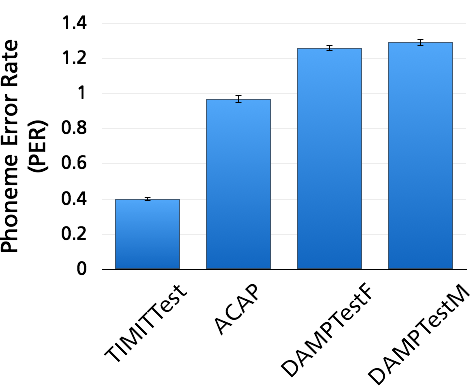
\includegraphics[width=\textwidth]{images/res_timit_per.png}
		\caption{Phoneme error rate}
		
	\end{subfigure}%
	\begin{subfigure}[c]{0.45\textwidth}
		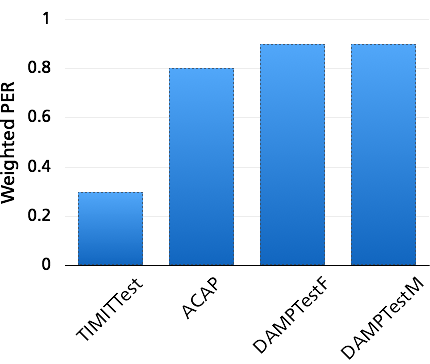
\includegraphics[width=\textwidth]{images/res_timit_wper.png}
		\caption{Weighted phoneme error rate}
	\end{subfigure}
	\caption{Mean phoneme recognition results on the test data sets using acoustic models trained on \textit{TIMIT}.}\label{fig:res_timit}
\end{figure*}



%\section{Phoneme recognition on synthesized singing}
% sinsy; female only
% dnn
%phonerec tested on:
% matched set, acap, dampf
%problem: correct instead of w_per!!
%A first idea to solve the lack of large singing data sets was the use of synthesized singing. For these experiments, the \textit{SYNTH} data set described in section \ref{subsec:data_synth}�was employed. As mentioned, this corpus contains vocal versions of pop songs synthesized with a female voice.\\
%A DNN of the same dimensions as before (1024x850x1024) was trained on the training portion, and then tested on the test portion of \textit{SYNTH}, on the \textit{ACAP} data set, and on the \textit{DAMPTest} sets. The results are displayed in figure \ref{fig:res_synth}.\\

%non-matched: not good (but better than timit??)
% not realistic; just a single voice
% audible accent

\section{Phoneme recognition using models trained on ``songified" speech}
% time stretch, pitch shift
% variants
% dnn vs dbn??
% phonerec tested on: timit, acap
% todo: test on damp

When there is a scarcity of suitable training data, attempts are often made to generate such data artificially from existing data for other conditions. For example, this is often done when models for noisy speech are required \cite{ntimit}\cite{aurora}. Inspired by this, one idea was making existing speech data sets more ``song-like'' and use these modified datasets to train models for phoneme recognition in singing. The \textit{TIMIT} corpus was once again used as a basis for this.\\

An overview of the approach is shown in figure \ref{fig:process_songify}. Five variants of the training part  \textit{TIMIT} were generated first. MFCC features were then extracted from these new datasets and used to train models.\\
Similarly, MFCCs are extracted from the \textit{TIMIT} Test set and from the \textit{ACAP} data set. The previously trained models are used to recognize phonemes on these test datasets. Viterbi decoding can then be used to generate phoneme sequences. Finally, the results are evaluated.

%TODO: check
\begin{figure*}
 \begin{center}
                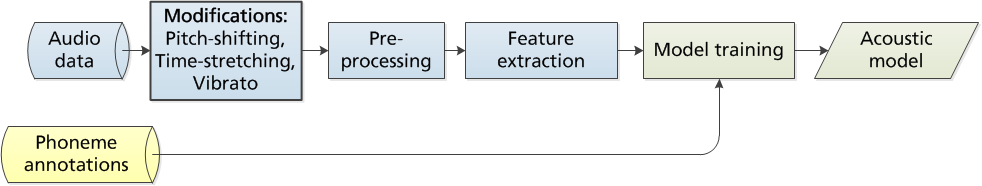
\includegraphics[width=1\textwidth]{images/process_training_phones_songify.png}
                \caption{Overview of the ``songified'' phoneme recognition training process.}
                \label{fig:process_songify}
                 \end{center}
 \end{figure*}
In order to make the training data more ``song-like'', several variants of this dataset were developed. Table \ref{tab:timit_variants} shows an overview over the five datasets generated from \textit{TIMIT} using three modifications. Dataset $N$ is the original \textit{TIMIT} training set. For dataset $P$, four of the eight blocks of \textit{TIMIT} were pitch-shifted. For dataset $T$, five blocks were time-stretched and vibrato was applied to two of them. In dataset $TP$, the same is done, except with additional pitch-shifting. Finally, dataset $M$ contains a mix of these modified blocks.\\
In detail, the modifications were performed in the following way:

\begin{description}
 \item[Time stretching] For time stretching, the phase vocoder from \cite{ellis_pvoc}, which is an implementation of the Flanagan/Dolson phase vocoder \cite{flanagan}\cite{dolson}, was used. This algorithm works by first performing a Short-Time Fourier Transform (STFT) on the signal and then resampling the frames to a different duration and performing the inverse Fourier transform.\\
 As demonstrated in section \ref{sec:sota_speechtosinging}, time variations in singing are mainly performed on vowels and are often much longer than in speech. Therefore, the \textit{TIMIT} annotations were used to only pick out the vowel segments from the utterances. They were modified randomly to a duration between $5$ and $100$ times the original duration and then re-inserted into the utterance. This effectively leads to more vowel frames in the training data, but since there is already a large amount of instances for each phoneme in the original training data, the effects of this imbalance should be negligible. 
 \item[Pitch shifting] To pitch-shift the signal, code from the freely available Matlab tool \textit{AutoTune Toy}\cite{autotunetoy}, which also implements a phase vocoder, was used. In this case, the fundamental frequency is first detected automatically. The signal is then stretched or expanded to obtain the new pitch and interpolated to retain the original duration.\\
 Using the \textit{TIMIT} annotations, utterances were split up into individual words, and then a pitch-shifted version of each word was generated and the results were concatenated. Pitches are randomly selected from a range between $60\%$ and $120\%$ of the original pitch.
 \item[Vibrato] The code for vibrato generation was also taken from \textit{AutoTune Toy}. It functions by generating a sine curve and using this as the trajectory for the pitch shifting algorithm mentioned above. A sine of amplitude $0.2$ and frequency 6Hz was used.\\
 In singing, vibrato is commonly done on long sounds, which are usually vowels. Since spoken vowels are usually very short, vibrato cannot be perceived on them very well. Therefore, vibrato was only added when time stretching was also applied. Vibrato was then added to the extracted and stretched vowels.
\end{description}



\begin{table}
 \begin{center}
  \begin{tabular}{|c||c|c|c|c|c|}
  \hline
   & \textbf{N} & \textbf{P} &\textbf{T} &\textbf{TP} &\textbf{M} \\
  \hline
  DR1 & N & N & N & N & N  \\
  DR2 & N & N & N & N & N \\
  DR3 & N & N & N & N & P\\
  DR4 & N & N & T & TP & TV \\
  DR5 & N & P & T & TP & TPV \\
  DR6 & N & P & T & TP & TV \\
  DR7 & N & P & TV & TPV & P \\
  DR8 & N & P & TV & TPV & TPV \\
  \hline
 \end{tabular}
\end{center}
 \caption{The five TIMIT variants that were used for training (rows are TIMIT blocks, columns are the five datasets).
  Symbols: N - Unmodified; P - Pitch-shifted; T - Time-stretched; V - Vibrato}
 \label{tab:timit_variants}
\end{table}


\begin{figure*}
	\centering
	\begin{subfigure}[c]{0.5\textwidth}
		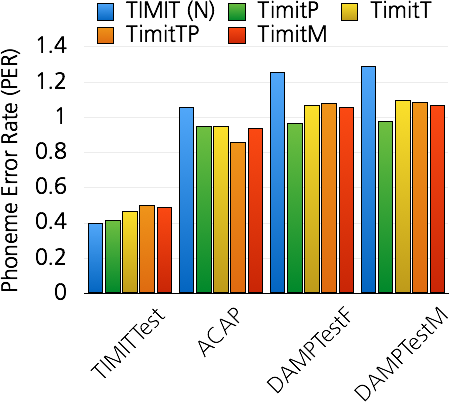
\includegraphics[width=\textwidth]{images/res_songify_per.png}
		\caption{Phoneme error rate}
		
	\end{subfigure}%
	\begin{subfigure}[c]{0.5\textwidth}
		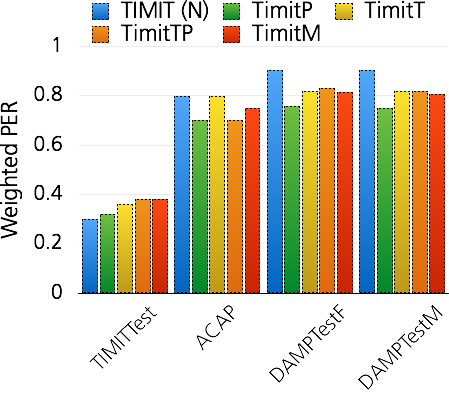
\includegraphics[width=\textwidth]{images/res_songify_wper.png}
		\caption{Weighted phoneme error rate}
	\end{subfigure}
	\caption{Mean phoneme recognition results on the test data sets using acoustic models trained on \textit{TIMIT} and augmented versions thereof.}\label{fig:res_songify}
\end{figure*}
The approach was tested on the various test data sets - namely, the test part of \textit{TIMIT}, the \textit{TIMIT} data set, and the two test sets chosen from the \textit{DAMP} data set. Figure \ref{fig:res_songify} shows the results for the DNN models. As it demonstrates, results for singing are generally worse than for speech. The base result for singing is a Weighted Phoneme Error Rate of $0.8$ for \textit{ACAP}, and of $0.9$ for both \textit{DAMPTestF} and \textit{DAMPTestM} (model trained on the original TIMIT dataset). When comparing the models trained on the various \textit{TIMIT} modifications, an improvement is observed for all variants. In contrast, none of the modifications improved the result on the speech data at all. The base result here $0.3$. (see previous section). This makes sense since all of the modifications make the training data less similar to the test data set.\\
On singing, the Weighted Phoneme Error rate falls by $0.1$ to $0.15$ when using models trained on the pitch-shifted data set (\textit{TimitP}), and by up to $0.08$ when using the time-stretched training data (\textit{TimitT}). The improvements for the corpora with both improvements lie in between. Vibrato does not appear to have a strong influence on the result. The higher error rates for \textit{DAMPTest} can, again, be explained with the fact that this data set has more variation in audio and singing quality.\\
%pitch shift: stronger, actual new feature values instead of just more; more realistic than long vowels because of shaping??
Pitch shifting might have a stronger effect on the recognition result because it is a stronger modification in the sense that it generates actual new feature values. In contrast, time stretching mostly generates new frames with values similar to the ones in the original data set (and only in between those). Additionally, pitch shifting may introduce more variety that is closer to sung sounds because singers do not usually shape long vowels just by stretching out their short versions.\\
Nevertheless, it is interesting to see that both pitch shifting and time stretching improve the result for sung phoneme recognition. This indicates that more variety in the training data is a step in the right direction. However, there is still a lot of room for improvement.





\section{Phoneme recognition using models trained on a-capella singing} \label{sec:phonerec_acap}
%how created?
% dnn
%phonerec tested on:
% acap, dampf/m
%alignment tested on acap; also: hmms!!
In this section, the most salient tested approach for phoneme recognition in singing is presented. For this method, acoustic models were trained on actual singing recordings. A large set of such recordings was already available from the \textit{DAMP} corpus, but no annotations were included with them. Such annotations were generated automatically from text lyrics available on the internet. In the following subsections, this process is described in detail, some variants are tested, and experiments with these new models are presented. 

\subsection{Corpus construction}\label{subsec:phonerec_corpus}



\begin{figure*}
 \begin{center}
                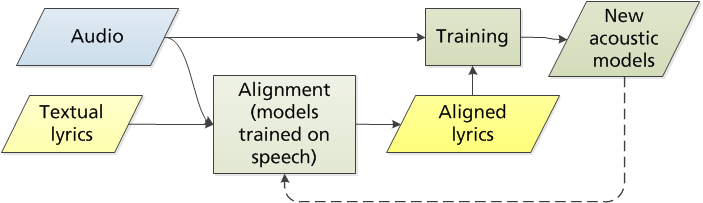
\includegraphics[width=.8\textwidth]{images/process_bootstrap.png}
                \caption{An overview of the alignment process. The dotted line represents the optional bootstrapping.}
                \label{fig:damp_alignment_process}
                 \end{center}
 \end{figure*}
 
As mentioned above, no lyrics annotations are available for the \textit{DAMP} data set, but the textual lyrics can be obtained from the \textit{Smule Sing!} website\footnote{\url{http://www.smule.com/songs}}.  All of them were English-language songs. These lyrics were mapped to their phonetic content using the CMU Pronouncing Dictionary\footnote{\url{http://www.speech.cs.cmu.edu/cgi-bin/cmudict}} with some manual additions of unusual words. As with the other data sets, this dictionary has a phoneme set of 39 phonemes (also see appendix \ref{app:phonemes}).\\
An automatic alignment of these lyrics to the \textit{DAMP} audio was then performed using the HMM acoustic models trained on \textit{TIMIT} (see section \ref{sec:phonerec_timit}). Viterbi alignment was performed on the word and phoneme levels using the HTK framework, using MFCCs and their deltas and double-deltas as features. This is the same principle of so-called ``Forced Alignment" that is commonly used in Automatic Speech Recognition \cite{book:jurafsky} (although it is usually done on shorter utterances). \\
Several different alignment strategies were carried out:
\begin{description}

\item[One state vs. three states per phoneme] Versions with one state per phoneme and three states per phoneme (so-called ``senones'', modeling the start, middle, and end phases) were tested. Since \textit{TIMIT} only contains single-phoneme annotations, this was done by first splitting the phoneme time frames evenly through three, and then re-training the \textit{TIMIT} acoustic model and re-aligning the data set (with the assumption that the transitions between the three states would be ``pulled'' to the correct times).  
\item[One-pass alignment vs. Bootstrapping] On top of a one-pass alignment using the Viterbi algorithm, bootstrapping the acoustic models to improve the alignment was also. To clarify: The alignment was first performed on the \textit{DAMP} data sets using the \textit{TIMIT} models described above, then acoustic models were trained on the resulting phoneme annotations. Then, those models were used to re-align the \textit{DAMP} data, which was again used to train another model. This was done over three iterations.\\
A modified version of the alignment algorithm was used for doing alignment with the models trained on the \textit{DAMP} data sets. This approach is based on doing Dynamic Time Warping on the generated phoneme posteriorgrams without punishing very long states. This is similar to the approach described in \ref{sec:ret_post}.
\end{description}
A graphical overview of the alignment process is given in figure \ref{fig:damp_alignment_process}.\\
Of course, errors cannot be avoided when doing automatic forced alignment. All in all, there were now four combinations of these strategies, which were compared. The next section describes how this alignment procedure was validated and what strategies performed best.\\
Since there is usually a large number of recordings of the same song, an approach using this information to improve the alignment results was also considered, e.g. by averaging time stamps over the alignments of several recordings. This was not done in this work because recordings tend to have different offsets from the beginning (i.e. silence in the beginning), and the singers also do not necessarily pronounce phonemes at the same time. This might be an avenue for future research, though.

%\subsection{Validation}\label{sec:validation}
%Validating the phoneme annotations created in this way is not trivial since there is no ground truth to base them on. Therefore, a two-pronged approach was employed: The same alignment algorithm was first tested on the small, manually annotated \textit{ACAP} data set. Second, new acoustic models were trained on the newly generated training data sets. Then, phoneme recognition was performed on the test data sets, and the results were compared to the expected phoneme strings (which are known from the matching lyrics).

\subsection{Alignment validation}
The alignment approach that was used to create the new \textit{DAMP}-based data sets was first tested on the \textit{ACAP} data set. To recap: This approach employs models trained on the \textit{TIMIT} speech corpus, which are used for Viterbi alignment of the known phonemes to the singing. The result of this is then compared to the manual annotations by calculating the difference between each expected and predicted phoneme transition. As mentioned in \ref{sec:phonerec_timit} and shown in figure \ref{fig:res_alignment}, the mean alignment error for this first approach is $0.16$ seconds for the three-state case, and $0.17$ for single phoneme states.\\

%TODO: other figure
\begin{figure}
	\begin{center}
		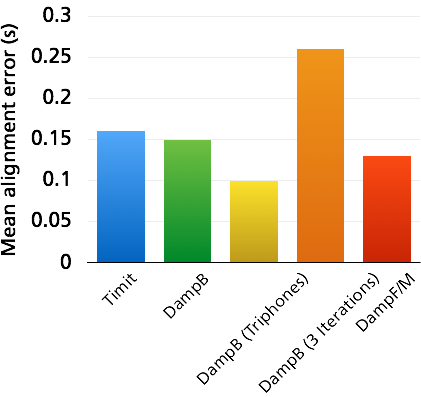
\includegraphics[width=.8\textwidth]{images/res_alignment.png}
		\caption{Mean alignment error in seconds on the \textit{ACAP} data set. \textit{TIMIT} shows the result for the same models used for aligning the new \textit{DAMP}-based data sets.}
		\label{fig:res_alignment}
	\end{center}
\end{figure}


Various models trained on the new \textit{DampB}, \textit{DampF}, and \textit{DampM} training data sets were then tested for the same task. The results are also shown in figure \ref{fig:res_alignment}.\\
Models trained on the monophonic alignments of \textit{DampB} perform slightly better at this task with mean errors of $0.15$ seconds. For the gender-specific models, the error was only calculated for the songs of the matching gender in \textit{ACAP}, resulting in the same average value. Since the gender-specific models do not produce better results, the other experiments were conducted on the mixed training set only. The three-state version of \textit{DampB} performs even better at alignment, with a mean error of $0.1$. This might happen because dedicatedly training the model for the start and end parts of phonemes might make the alignment approach more accurate at finding start and end points.\\
Finally, a model trained on \textit{DampB} over three iterations was also tested for alignment. This model performs much worse at this task with a mean alignment error of $0.26$. This might happen because errors in the original alignment of the phonemes may become amplified over these iterations. The effect is not as pronounced for the three-state version, but it is still present.


\begin{figure*}
	\centering
	\begin{subfigure}[c]{0.5\textwidth}
		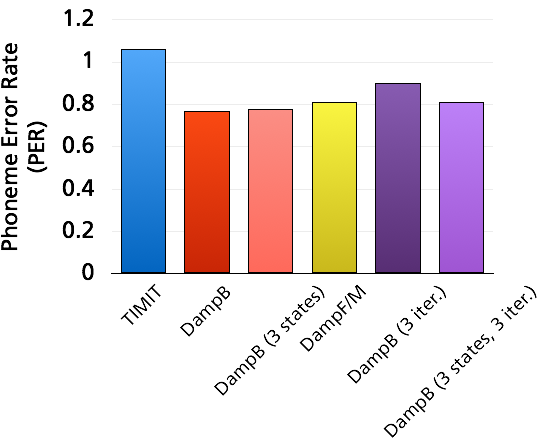
\includegraphics[width=\textwidth]{images/res_phonerec_acap.png}
		\caption{Phoneme error rate}
		
	\end{subfigure}%
	\begin{subfigure}[c]{0.5\textwidth}
		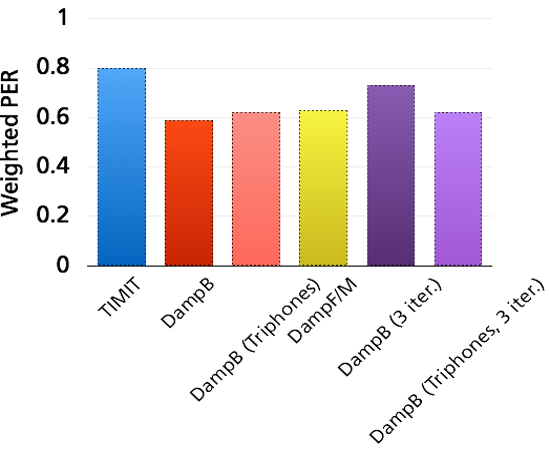
\includegraphics[width=\textwidth]{images/res_phonerec_acap_w.png}
		\caption{Weighted phoneme error rate}
	\end{subfigure}
	\caption{Mean phoneme recognition results on the \textit{ACAP} data set using acoustic models trained on \textit{Timit} and the new \textit{DAMP}-based data sets.}\label{fig:res_phonerec_acap}
\end{figure*}

\begin{figure*}
	\centering
	\begin{subfigure}[c]{0.5\textwidth}
		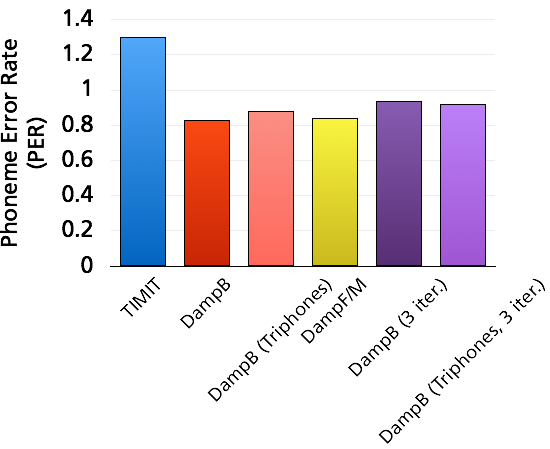
\includegraphics[width=\textwidth]{images/res_phonerec.png}
		\caption{Phoneme error rate}
		
	\end{subfigure}%
	\begin{subfigure}[c]{0.5\textwidth}
		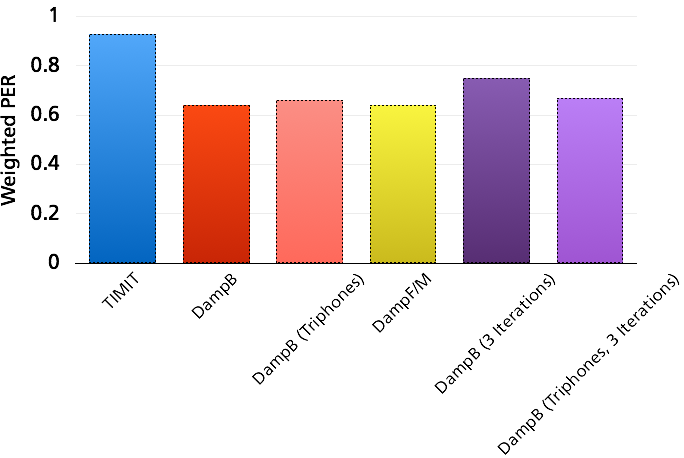
\includegraphics[width=\textwidth]{images/res_phonerec_w.png}
		\caption{Weighted phoneme error rate}
	\end{subfigure}
	\caption{Mean phoneme recognition results on the \textit{DampTest} data sets using acoustic models trained on \textit{TIMIT} and the new \textit{DAMP}-based data sets.}\label{fig:res_phonerec}
\end{figure*}


\begin{figure*}
	\centering
	\begin{subfigure}[c]{0.5\textwidth}
		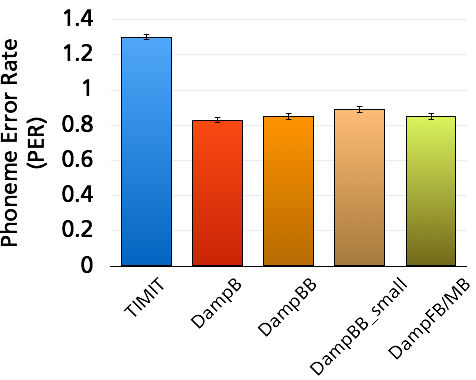
\includegraphics[width=\textwidth]{images/res_phonerec_sizes.png}
		\caption{Phoneme error rate}
		
	\end{subfigure}%
	\begin{subfigure}[c]{0.5\textwidth}
		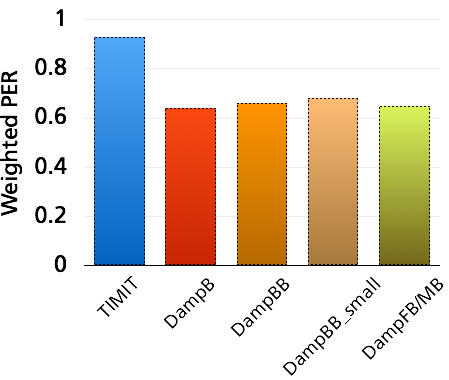
\includegraphics[width=\textwidth]{images/res_phonerec_sizes_w.png}
		\caption{Weighted phoneme error rate}
	\end{subfigure}
	\caption{Mean phoneme recognition results on the \textit{DampTest} data sets using acoustic models trained on \textit{TIMIT} and the new \textit{DAMP}-based data sets.}\label{fig:res_phonerec_sizes}
\end{figure*}

\subsection{Phoneme recognition}
After validating the alignment strategy, phoneme recognition experiments were performed on both the \textit{ACAP} and the \textit{DampTest} corpora. This was possible even though there are no manual annotations for the \textit{DampTest} sets because the expected phonemes are available from the textual lyrics. Again, the phoneme error rate and the weighted phoneme error rate were used as evaluation measures (see \ref{subsec:tech_systems_phonerec}).\\
The results for \textit{ACAP} are shown in figure \ref{fig:res_phonerec_acap}. In general, models trained on \textit{DampB} performed much better at phoneme recognition than those trained on \textit{TIMIT}. Compared to these speech-based models, the phoneme error rate falls from $1.06$ to $0.77$, while the weighted phoneme error rate falls from $0.8$ to $0.59$. As can be seen from both evaluation measures, using alignments with three states per phoneme instead of single states does not improve the results in this case, contrasting with the better alignment results. This might happen because more classes cause more confusion in the model, even though the three-state results were downmapped to single phonemes for calculating the evaluation measures. Additionally, the temporal pronunciation phases may just be too variable in singing, as opposed to speech. As in the alignment results, using gender-specific models does not provide an advantage over a mixed model. (Results for the gender-specific models were only evaluated on songs of the matching gender).\\
As already seen in the alignment validation results, training models on \textit{DampB} over three iterations actually degrades the result. Again, this might happens because phoneme alignment errors become amplified in this way. Interestingly, the effect is not as strong for the three-state models, perhaps because the three classes per phoneme help to alleviate each other's errors.\\

The results for the same procedure on the \textit{DampTest} sets are shown in figure \ref{fig:res_phonerec}. Results over \textit{DampTestF} and \textit{DampTestM} were averaged.
The same general trend can be observed for these results: The phoneme error rate falls from $1.3$ to $0.83$ when compared to models trained on \textit{TIMIT}, with the weighted phoneme error rate decreasing from $0.93$ to $0.64$. Using three states per phoneme does not contribute to the result, and neither does the three-iteration bootstrapping process for training acoustic models. As in the \textit{ACAP} results, not even the gender-specific models improve the result. This effect might occur because the range of pitch and expressions is much wider in singing than in speech, and therefore gender-specific models may not actually learn as much added helpful information. Other experiments indicated that gender-specific models also do not improve the results when using three states or three alignment iterations as with the mixed-gender training data.\\

Going forward, single-state models trained on mixed-gender data (i.e. \textit{DampB}) appear to be the best and simplest solution. To gain insight into the role of the composition of the training data set, more experiments were conducted with the variants of \textit{DampB} described in section \ref{sec:data_damp}. The results are shown in figure \ref{fig:res_phonerec_sizes}.\\

When using the smaller, more balanced version of \textit{DampB} (\textit{DampBB}), the results become somewhat worse, but not much, with a phoneme error rate of $0.85$, and a weighted phoneme error rate of $0.66$. This is particularly interesting because this data set is only 4\% the size of the bigger one and training is therefore much faster. With the smallest data set which is only half the size of \textit{DampBB}, the change is similar: The Phoneme Error Rate rises to $0.89$, the Weighted Phoneme Error Rate to $0.68$. Since this data set has roughly the same amount of phonemes as \textit{TIMIT}, this proves that the improvement is actually caused by the acoustic properties of the training data, rather than just the larger amount of data. (Of course, this factor also contributes). The reduced versions of \textit{DampF} and \textit{DampM} were tested as well, but once again, they do not provide an improvement over the mixed gender model.\\


\subsection{Error sources}\label{subsec:error_sources}
Of course, with an automatic alignment algorithm like this, errors cannot be avoided. To acquire a clearer picture of the reasons for the various misalignments, the audio data where they occurred was analyzed more closely. Some sources of error repeatedly stuck out:
%\begin{compactdesc}
\begin{description}
 \item[Unclear enunciation]{Some singers pronounced words very unclearly, often focusing more on musical performance than on the lyrics.}
 \item[Accents]{Some singers sung with an accent, either their natural one or imitating the one used by the original singer of the song.}
 \item[Young children's voices]{Some recordings were performed by young children.}
 \item[Background music]{Some singers had the original song with the original singing running in the background.}
 \item[Speaking in breaks]{Some singers spoke in the musical breaks.}
 \item[Problems in audio quality]{Some recordings had qualitative problems, especially loudness clipping.}
%\end{compactdesc}
\end{description}
For most of these issues, more robust phoneme recognizers would be helpful. For others, the algorithm could be adapted to be robust to extraneous recognized phonemes (particularly for the speaking problem). If possible, a thorough manual check of the data would be very helpful as well.



\section{Conclusion}
% timit starting point
% songified somewhat better (what?)
% best: actual singing
% problem: no annotations
% solution: get text lyrics, align with timit models; alignment verified on acap
% best results on speech (easiest)
% acap better than damp test sets
% because: better enunciation, homogenous recording quality, fewer annotation errors (!!)
% gender-specific not helpful
%triphones sometimes help, sometimes not
% iterating amplifies errors
% decimating training data still produces good models
% overtraining???
% error sources
In this chapter, new approaches for phoneme recognition in singing were described. As a starting point, DNN models were trained on the \textit{TIMIT} speech corpus. For verification, these models were evaluated on the test section of \textit{TIMIT}, resulting in a Phoneme Error Rate of $0.4$ and a Weighted Phoneme Error Rate of $0.3$. The results on the \textit{ACAP}�singing data set were much worse: A Phoneme Error Rate of $1.06$ and a Weighted Phoneme Error Rate of $0.8$, demonstrating the difficulty of phoneme recognition in singing as opposed to speech. Similarly, the Phoneme Error Rate was $1.28$ on the \textit{DampTest} data sets, with a Weighted Phoneme Error Rate of $0.9$. Generally, results on the \textit{DampTest} sets are worse than on the \textit{ACAP} test set, which presumably happens because the \textit{DampTest} sets are performed by amateurs, whose enunciation is not as clear as that of the professional singers in the \textit{ACAP} set and who may not always sing the correct lyrics, because the recording quality varies much more, and because the annotations may contain errors due to the automatic phoneme alignment (as opposed to the more realiable manual annotations of \textit{ACAP}).\\

In order to make the models better adapted to singing, acoustic modifications were performed on the \textit{TIMIT} training data - namely, pitch shifting and time stretching. This increases the Phoneme Error Rate on speech test data (\textit{TIMITTest}, but improves them on sung data. Pitch shifting appears to have a stronger effect than time stretching, which might happen because this modification results in actual changed feature data, whereas time stretching mainly produces more frames with feature values similar or in between the existing ones. On the \textit{ACAP} test data, the lowest Phoneme Error Rate is $0.95$, and the lowest Weighted Phoneme Error Rate is $0.7$ (with the pitch-shifted models). On \textit{DampTest}, those values are decreased to $0.98$ and $0.76$ respectively.\\

The best-adapted models for recognizing phonemes in singing should be those trained on actual singing data. Unfortunately, there are no big, annotated singing data sets like those for speech. For this reason, the \textit{DAMP} data set, which contains thousands of recordings of unaccompanied amateur singing, was selected, and the text lyrics were obtained from the internet. Then, various strategies for aligning the phonetic content of these lyrics to the audio were tested. In the simplest algorithm, HMM models trained on \textit{TIMIT} were used for Viterbi alignment. This also turned out to be one of the most effective algorithms for the alignment process necessary for constructing this new singing data set.\\

The resulting annotations, together with the singing audio data, were then used to train new DNN models for phoneme recognition. Using 6000 of these recordings of singers of both genders, the Phoneme Error Rate was lowered to $0.77$ on the \textit{ACAP} test set, and the Weighted Phoneme Error Rate was lowered to $0.59$. On the \textit{DampTest} sets, those values decreased to $0.83$ and $0.64$ respectively. Neither employing three states per phoneme instead of a single state nor training gender-specific models provided additional advantages. Iterating the alignment process decreased the result, possibly because errors in the original alignment become amplified over these iterations.\\

The influence of training set size was also investigated on the \textit{DampTest} data. Using a phonetically balanced subset of \textit{DAMP} that was just $4\%$ of the size of the originally selected training set worsened the result by only 2 percent points (both in Phoneme Error Rate and Weighted Phoneme Error Rate). Using an even smaller data set that is roughly the size of \textit{TIMIT} increased the Phoneme Error Rate only by a further 4 percent points (and the Weighted Phoneme Error Rate by 2), thereby proving that the better recognition results are caused by the sung content rather than just the size of the training data.\\
%OVERTRAINING???

%!!!
A manual error analysis was performed on cases where the phoneme recognition failed. Errors are frequently caused by linguistically or acoustically difficult segments in the test data, such as accents, children's voices, background music, or additional speaking.\\

Comparing these results to the state of the art is difficult because of the different testing data used. Considering raw numbers, it can be assumed that the best results are in the range of the best state of the art results, for example those by Mesaros et al. \cite{Mesaros2011} (see section \ref{sec:sota_phonerec}). In contrast to these approaches, no involved post-processing is employed. In the future, integrating such steps as singer adaptation and language modeling would in all probability serve to improve the approach even more.\\
Another option that has not been tested yet is the use of triphones (i.e. training tied models for phonemes with context dependency on their predecessors and successors). This approach is frequently used in ASR.




%TODO: Erw�hnen, welche balancierten Subsets genutzt wurden

\chapter{Sung Language Identification} \label{chap:langid}
%Sung language identification is the task of automatically determining the language of a sung recording. For this task, two algorithms were developed: One based on i-vector extraction, and one based on analysis of the statistics of phoneme posteriorgrams. They will be described in detail in this chapter.\\
%In both cases, the \textit{NIST2003LRE} and \textit{OGIMultilang} corpora were used for testing the algorithms on speech, and the \textit{YTAcap} data set was used for singing (see chapter \ref{chap:datasets}).
\begin{figure}
	\begin{center}
		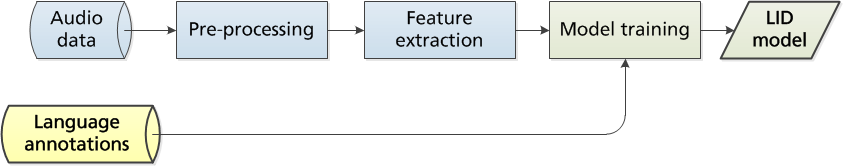
\includegraphics[width=1\textwidth]{images/process_training_lid.png}
		\caption{Schematic of the training procedure for language identification.}
		\label{fig:process_training_lid}
	\end{center}
\end{figure}
\begin{figure}
	\begin{center}
		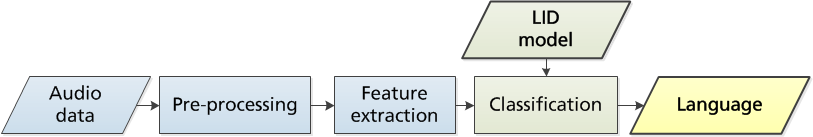
\includegraphics[width=1\textwidth]{images/process_classification_lid.png}
		\caption{Schematic of the classification procedure for language identification.}
		\label{fig:process_classification_lid}
	\end{center}
\end{figure}

Language identification has been extensively researched in the field of Automatic Speech Recognition since the 1980's. A number of successful algorithms has been developed over the years. An overview over the fundamental techniques is given by Zissman in \cite{zissman}.\\
Fundamentally, four properties of languages can be used to discriminate between them:
\begin{description}
	\item[Phonetics] The unique sounds that are used in a given language.
	\item[Phonotactics] The probabilities of certain phonemes and phoneme sequences.
	\item[Prosody] The ``melody'' of the spoken language.
	\item[Vocabulary] The possible words made up by the phonemes and the probabilities of certain combinations of words.
\end{description}
Even modern systems mostly focus on phonetics and phonotactics as the distinguishing factors between languages. Vocabulary is sometimes exploited in the shape of language models.\\
In ASR, the standard technique for language identification is Parallel Phone Recognition followed by Language Modeling (PPRLM). In this approach, acoustic and language models are trained for each language (or, in some cases, only the language models are different and just one acoustic model is used) . Unseen examples are then run through each model or combinations thereof, and the result with the highest likelihood determines the language (e.g. \cite{lid_li_ma} and \cite{lid_matejka}).\\
Other approaches directly train models for each language on the feature vectors (e.g. GMMs). This technique can be considered a ``bag of frames'' approach, i.e. the single data frames are considered to be statistically independent of each other. The trained models then describe probability densities for certain acoustic characteristics of each language. GMM approaches used to perform worse than their PPRLM counterparts, but the development of new features has made the difference negligible \cite{singer}. They are, in general, easier to implement since only audio examples and their language annotations are required. Allen et al. \cite{allen} report results of up to $76.4\%$ accuracy for ten languages. Different backend classifiers, such as Multi-Layer Perceptrons (MLPs) and Support Vector Machines (SVMs) \cite{campbell}, have also been used successfully instead of GMMs.\\
%HERE??
In this work, an approach that trains directly on the acoustic characteristics using i-vector extraction and SVMs is presented. The modifications to the general processing chain are presented in figures \ref{fig:process_training_lid} and \ref{fig:process_classification_lid}.\\
 
Additionally, a second approach based on phoneme posteriorgrams is tested. Statistics from the posteriorgrams are calculated, and then a second model is trained on these. Similar methods have been developed in ASR: Berkling presented an approach that uses sequences of recognized phonemes to discriminate between two languages (English and German), either with statistical modeling or with Neural Networks \cite{phdthesis:berkling_phd}. Mean errors of $0.12$ and $0.07$ on unseen data are achieved for the statistical approach and the Neural Network approach respectively when enough training data is available.\\
Li, Ma, and Lee present a system where acoustic inputs are tokenized into acoustic words, which do not necessarily correspond to phonetic n-grams. Then, language classifiers are trained on statistics of the acoustic words \cite{lid_li_ma_lee}. They obtain an equal error rate of $0.05$ for six languages using a universal phoneme recognizer for tokenization and SVMs for backend language recognition. Peche et al. \cite{peche} attempt a similar approach on languages with limited resources. The performance remains good even when only acoustic models trained on different languages are used.\\
In all of these approaches, tokenization of some sort is performed using the acoustic models. Since phoneme recognition on singing is still relatively unreliable, statistics are calculated directly on the phoneme posteriors in this work.\\


For evaluation, all test examples are classified into exactly one language class. Then, the accuracy (i.e. the average retrieval) is calculated:
 \begin{equation}
    Accuracy = \frac{TP}{N}
 \end{equation}  
 where $TP$ are the True Positives, and $N$ is the number of all documents. In ASR, the average cost measure as recommended in \cite{nist_cavg} is also used widely now; however, to remain in line with other sung language identification approaches such as those described in chapter \ref{chap:sota}, the accuracy was still used in this work.\\
 
 In both approaches, the \textit{NIST2003LRE} and \textit{OGIMultilang} corpora were used for testing the algorithms on speech, and the \textit{YTAcap} data set was used for singing (see chapter \ref{chap:datasets}).



\section{Sung language identification using i-vectors}
%known speakers - unknown speakers - whole documents


As described in section \ref{subsec:tech_ivector}, i-vector extraction is a feature dimension reduction technique that was originally developed for speaker recognition, but has since then been employed successfully for other tasks, including language identification. After the publication of this approach for i-vector extraction for sung language identification, it also started being used for other MIR tasks, such as artist recognition and similarity calculation \cite{eghbal-zadeh1}\cite{eghbal-zadeh2}.

\subsection{Proposed system}
\label{sec:system}
Figure \ref{fig:lid_ivectors} shows a rough overview over the i-vector classification system. 
%\begin{figure}[ht]
%\centerline{\includegraphics[scale=0.3]%{overview.png}}
%\caption{\label{fig:overview}{\it Overview of the steps of our classification system.}}
%\end{figure}
\begin{figure*}
	\begin{center}
		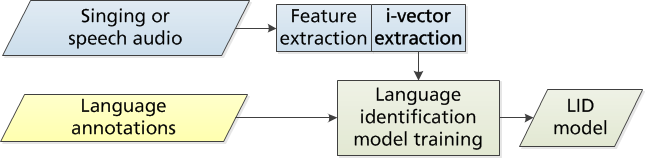
\includegraphics[width=.7\textwidth]{images/lid_ivectors.png}
		\caption{Overview of the process for language identification using i-vector extraction.}
		\label{fig:lid_ivectors}
	\end{center}
\end{figure*}

A number of features were extracted from each audio file. Table \ref{tab:ivec_configs} shows an overview over the various configurations used in training.
\begin{table}[h!tbp]
\scriptsize
  \begin{center}
     \begin{tabular}{|c|c|c|}\hline
     Name & Description & Dimensions \\ \hline
      MFCC  & MFCC, 20 coefficients & 20 \\
      MFCCDELTA  & MFCC, 20 coefficients, deltas and double-deltas & 60 \\
      MFCCDELTASDC  & MFCCDELTA+SDC & 117 \\
      SDC  & SDC with configuration $7-1-3-7$ & 91 \\
      RASTA-PLP & PLP with RASTA processing, model order 13 with deltas and double-deltas & 39 \\
      RASTA-PLP36  & PLP with RASTA processing, model order 36 with deltas and double-deltas  & 96 \\
      PLP  & PLP without RASTA processing, model order 13 deltas and double-deltas  & 39 \\
      COMB & PLP+MFCCDELTA & 99 \\ \hline
    \end{tabular}
  \end{center}
    \caption{{Feature configurations used in language identification training.}}
  \label{tab:ivec_configs}
\end{table}

For classification, Multi-Layer Perceptrons (MLPs) and Support Vector Machines (SVMs) are tested. The MLPs are fixed at three layers, with the middle layer having a dimension of 256. Additional layers do not seem to improve the result. A larger middle layer only improves it slightly. The SVM parameters are determined using a grid-search. For each of those classifiers and data sets, all feature combinations listed in table \ref{tab:ivec_configs} are tested directly and with i-vector processing. All results are obtained using five-fold cross validation. \\


\subsection{Experiments with known speakers}
In the first experiment, MLP and SVM models are trained on randomly selected folds of the training data sets. This means that recordings by the same speaker are spread out between the training and test data sets. In theory, i-vectors could be particularly susceptible to capturing speaker characteristics instead of language characteristics, leading to evaluation results that may not be representative of results for unknown speakers. However, this effect is often ignored in literature \cite{Martin2010}, and an argument can be made that partially training models on speaker properties is realistic for some use cases (i.e. when many of the expected speakers for each language are already known).\\

\begin{figure}[h]
       \centering
      \begin{subfigure}[c]{0.3\textwidth}
                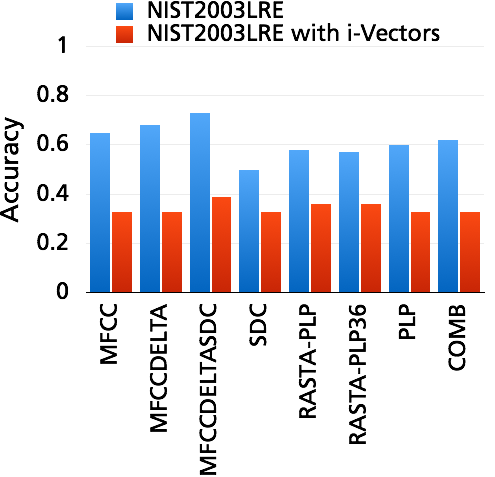
\includegraphics[width=\textwidth]{images/lid_exp1_nist.png}
                \caption{NIST2003LRE}
                \label{fig:lid_exp1_nist}
        \end{subfigure}%
        \begin{subfigure}[c]{0.3\textwidth}
                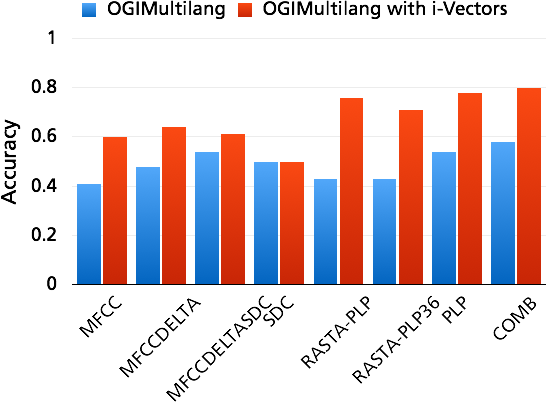
\includegraphics[width=\textwidth]{images/lid_exp1_ogi.png}
                \caption{OGIMultilang}
                \label{fig:exp1_ogi}
        \end{subfigure}
                \begin{subfigure}[c]{0.3\textwidth}
                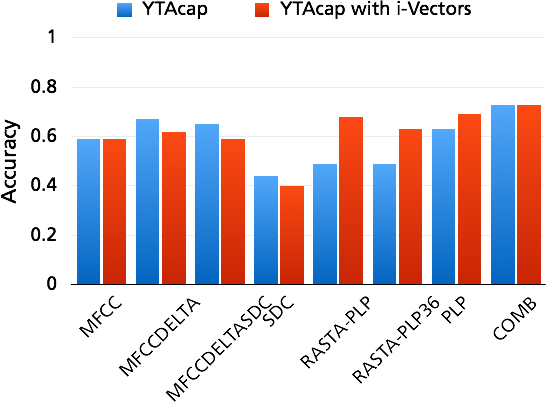
\includegraphics[width=\textwidth]{images/lid_exp1_yt.png}
                \caption{YTAcap}
                \label{fig:exp1_yt}
        \end{subfigure}
        \caption{Results using MLP models on all three language identification data sets, with or without i-vector processing.}\label{fig:lid_exp1}
\end{figure}

The results for the MLP training on the \textit{NIST2003LRE}, \textit{OGIMultilang}, and \textit{YTAcap} data sets are shown in figure \ref{fig:lid_exp1} in terms of accuracy (average retrieval when all documents are classified into exactly one language). \\
As shown in figure \ref{fig:lid_exp1_nist}, the MLP does not produce good results on the \textit{NIST2003LRE} database for any of the feature combinations. \textit{NIST2003LRE} is the smallest of the data sets by a large margin. Since a relatively high-dimensional model is used, this is probably a case of overtraining. The i-vector processing step reduces the training data even further, thus aggravating the problem.\\
The \textit{OGIMultilang} data set contains roughly 4 times as much data as the \textit{NIST2003LRE} set. With enough data, training an MLP classifier works a lot better. Without i-vector processing, this approach still only reaches about 52\% accuracy. i-Vector extraction improves the system massively. The best feature configurations are RASTA-PLP (82\%), PLP (80\%), and COMB (80\%).\\
As with all other experiments, the task becomes harder when attempted on singing data. The results on the \textit{YTAcap} data set are somewhat worse than those on \textit{OGIMultilang}, even though they contain a similar amount of data. The best result without i-vector extraction is still obtained using the COMB feature configuration at 56\% accuracy. Similar to the \textit{OGIMultilang} experiment, i-vector extraction yields a large improvement. COMB remains the best configuration, now at 77\% accuracy.\\

\begin{figure}[h]
       \centering
      \begin{subfigure}[c]{0.3\textwidth}
                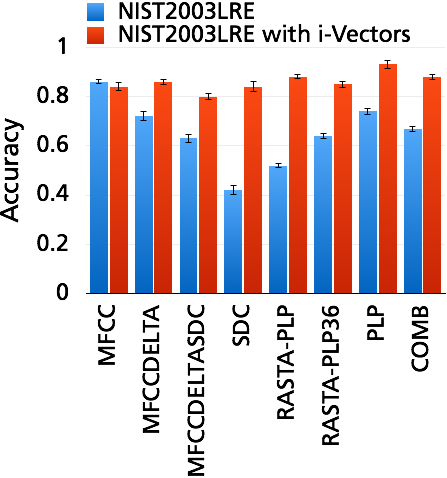
\includegraphics[width=\textwidth]{images/lid_exp1a_nist.png}
                \caption{NIST2003LRE}
                \label{fig:lid_exp1a_nist}
        \end{subfigure}%
        \begin{subfigure}[c]{0.3\textwidth}
                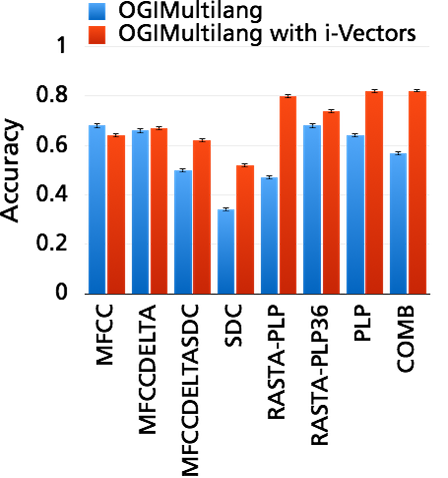
\includegraphics[width=\textwidth]{images/lid_exp1a_ogi.png}
                \caption{OGIMultilang}
                \label{fig:exp1a_ogi}
        \end{subfigure}
                \begin{subfigure}[c]{0.3\textwidth}
                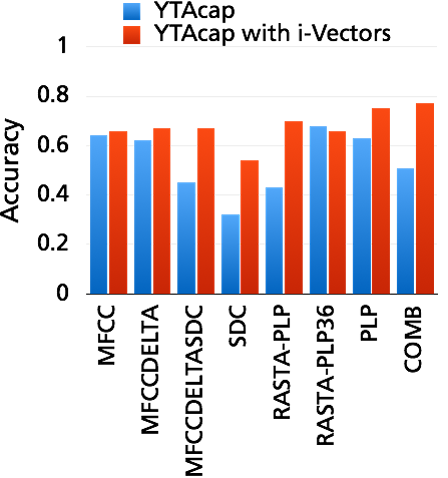
\includegraphics[width=\textwidth]{images/lid_exp1a_yt.png}
                \caption{YTAcap}
                \label{fig:exp1a_yt}
        \end{subfigure}
        \caption{Results using SVM models on all three language identification data sets, with or without i-vector processing, with speakers shared between training and test sets.}\label{fig:lid_exp1a}
\end{figure}


Figure \ref{fig:lid_exp1a} shows the results for the SVM models trained on the same data sets. In general, these models appear to be able to capture the language boundaries better.\\
In contrast to the MLP experiment, SVMs produce good results on the \textit{NIST2003LRE} data set for all of the features. They seem to be able to discriminate very well on this small, clean data set. The best result with i-vector processing is $86\%$ accuracy for MFCC features. When using i-vectors, a 93\% accuracy is achieved with PLP features. This may, in fact, be close to the upper bound for the classification here, which might be caused by annotation errors or ambiguous data.\\
The \textit{OGIMultilang} corpus is bigger and more varied than the \textit{NIST2003LRE} corpus, which makes it harder to classify. As shown, the high-dimensional pure features do not perform as well, with a maximum accuracy of 68\% for MFCCs and RASTA-PLPs with 36 coefficients. Using i-vector extraction improves the result by a large margin. Feature-wise, PLPs without RASTA processing work best at a result of 82\% accuracy. 
%CHECK!!!
MFCC and SDC features did not work quite as well, but did not hurt the result either when combined with PLPs (COMB result). It is interesting to see that the i-vector extraction decreased the results for MFCCs, the feature that worked best without it.\\
%CHECK!!
Similar to the \textit{OGIMultilang} corpus, the \textit{YTAcap} corpus provides very complex and varied data. The same effects occur with the direct feature training here, too: RASTA-PLPs with 36 coefficients provide the best results, but the accuracy is not very high at 68\%. i-Vector extraction once again serves to improve the result. The highest results when using i-vector extraction is a 75\% accuracy when using PLP without RASTA processing, or 77\% for the COMB configuration.

\subsection{Experiments with unknown speakers}

In order to find out what influence the speaker characteristics had on the result, the same experiments were then repeated with training and evaluation sets that strictly separated speakers. This experiment was not performed for the \textit{NIST2003LRE}�corpus because no speaker information is available for it. Since the SVM models performed better in the previous experiment, only these models were tested.\\

\begin{figure}[h]
       \centering
        \begin{subfigure}[c]{0.4\textwidth}
                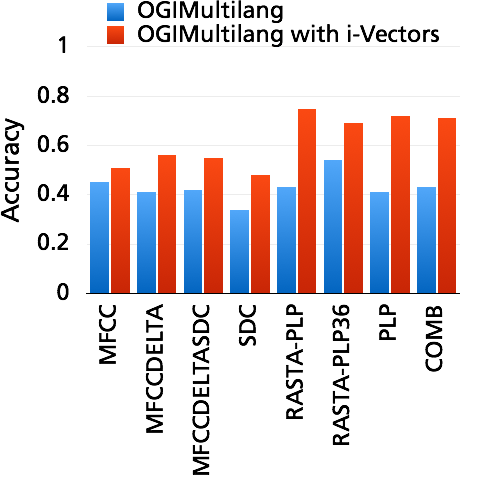
\includegraphics[width=\textwidth]{images/lid_exp2_ogi.png}
                \caption{OGIMultilang}
                \label{fig:exp2_ogi}
        \end{subfigure}
                \begin{subfigure}[c]{0.4\textwidth}
                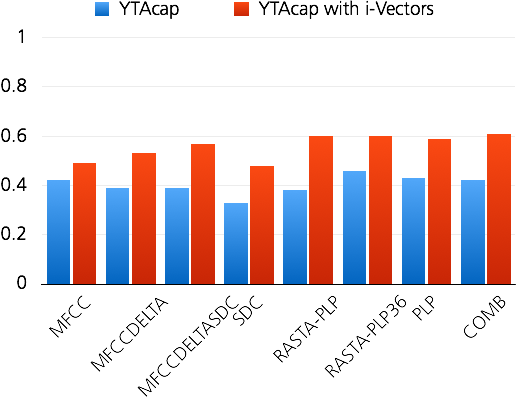
\includegraphics[width=\textwidth]{images/lid_exp2_yt.png}
                \caption{YTAcap}
                \label{fig:exp2_yt}
        \end{subfigure}
        \caption{Results using SVM models, with or without i-vector processing, with speakers separated between training and test sets.}\label{fig:lid_exp2}
\end{figure}

The results are shown in figure \ref{fig:lid_exp2}. In general, all configurations perform worse, indicating that some of the characteristics learned by the models come from the speakers rather than the languages. Apart from this, the general trends for the features remain the same, and i-vector extraction still improves the over-all results.\\

On the \textit{OGIMultilang} corpus, the best result is still obtained with RASTA-PLP features and i-vector processing, but the accuracy falls by around 8 percent points to $75\%$. On \textit{YTAcap}, the effect is even worse: From an accuracy of $77\%$ with the mixed condition, the result decreases to $61\%$ for the separated condition. The reason for this is probably the wider signal variety in singing as opposed to speech; additionally, \textit{YTAcap} also possesses a wider range of recording conditions than the controlled telephone conditions of \textit{OGIMultilang}. Arguably, the solution for this effect would be the use of larger training data sets, which would be able to cover these acoustic and performance conditions better. Conversely, as the previous results show, the approach produces better results when an application scenario can be limited to a range of known speakers, or at least recording conditions (as in the \textit{NIST2003LRE} experiment).


%TODO: info about speakers and material per speaker
\subsection{Experiments with utterances combined by speakers}

All previous experiments were performed on relatively short utterances of a few seconds in duration. In many application scenarios, much more audio data is available to make a decision about the language. In particular, songs are usually a few minutes in length, and in many cases, only one result per document (= song) is required.\\
For this reason, results for the \textit{YTAcap} data set are taken from the previous experiment and a majority voting decision is made for each song (and therefore also for each singer). For the \textit{OGIMultilang} corpus, results for all utterances by the same speaker are aggregated in the same fashion, resulting in similar durations of audio. (Again, this experiment was not performed with the \textit{NIST2003LRE} corpus due to the lack of speaker information).\\

\begin{figure}[h]
       \centering
           \begin{subfigure}[c]{0.4\textwidth}
                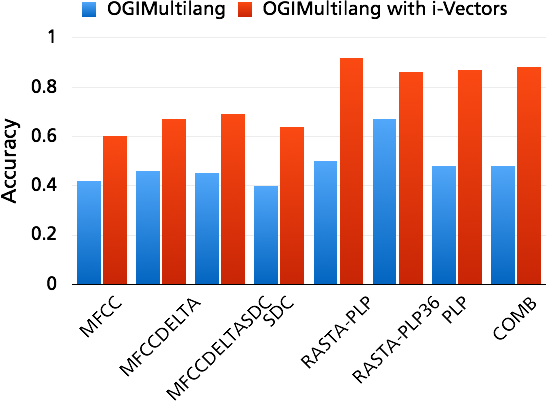
\includegraphics[width=\textwidth]{images/lid_exp3_ogi.png}
                \caption{OGIMultilang}
                \label{fig:exp3_ogi}
        \end{subfigure}
                \begin{subfigure}[c]{0.4\textwidth}
                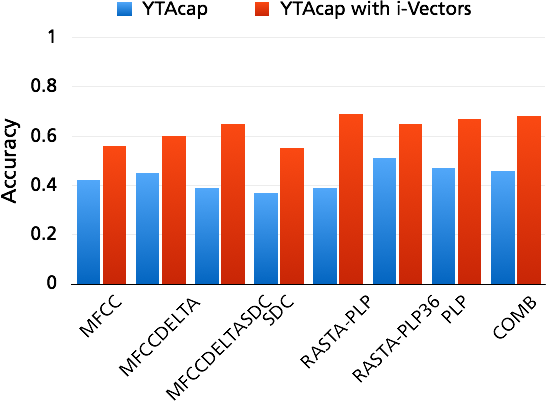
\includegraphics[width=\textwidth]{images/lid_exp3_yt.png}
                \caption{YTAcap}
                \label{fig:exp3_yt}
        \end{subfigure}
        \caption{Document-wise results using SVM models, with or without i-vector processing.}\label{fig:lid_exp3}
\end{figure}

The results are shown in figure \ref{fig:lid_exp3}. Overall, aggregation of multiple utterances by the same speakers seems to balance out some of the speaker-specific effects seen in the previous experiment. Taking more acoustic information into account, the models are able to determine the language with higher accuracy.\\
On the \textit{OGIMultilang} corpus, the result is even better than on the condition with known speakers. The best result rises from $75\%$ accuracy for short utterances to $92\%$ for the aggregated documents (both with the RASTA-PLP feature). On the \textit{YTAcap} data sets, the aggregated result is $69\%$ (compared to $60\%$ for line segments).\\

As suggested in the previous section, the approach produces results that are usable in practice when the problem can be narrowed down, e.g. to known speakers or recording conditions. As this experiment shows, useful results can also be obtained when longer sequences are available for analysis. 


\

%nicht n�tig f�r nist - kleine datenmengen gehen so mit svm. bei mlp aber overfitting.
%ogi: ivec erh�ht Ergebnis massiv. besser als irmfsp (warum?)
%yt: �hnlich ogi. Ergebnisse > sota. 
%features: plp gut, am besten ohne Rasta (warum?). mehr coeffs bringen aber nichts. mfcc f�r sich auch gut, mit delta noch besser, teilweise auch mit sdc.
%combi aus plp_norasta und mfccdelta funktioniert am besten - 2 verschiedene Aspekte abgedeckt (warum?)
%insgesamt: schnelleres training und weniger Speicherplatz als volle features, Irrelevanz reduziert. �hnliche Ergebnisse wie pprlm, aber viel einfacher. weniger Annotationen und leichter zu implementieren.




\section{Sung language identification using phoneme recognition posteriors}\label{sec:lid_stats}
Another developed approach is based upon phoneme statistics derived from phoneme posteriorgrams. To obtain representative statistics for model training, relatively long observations are necessary, but, as described in the previous section, this is the case for many applications, for example when considering song material (e.g. songs of 3-4 minutes in duration). On the other hand, phoneme posteriorgrams need to be calculated for a number of other tasks, such as keyword spotting or lyrics-to-audio alignment. \\

\begin{figure*}
	\begin{center}
		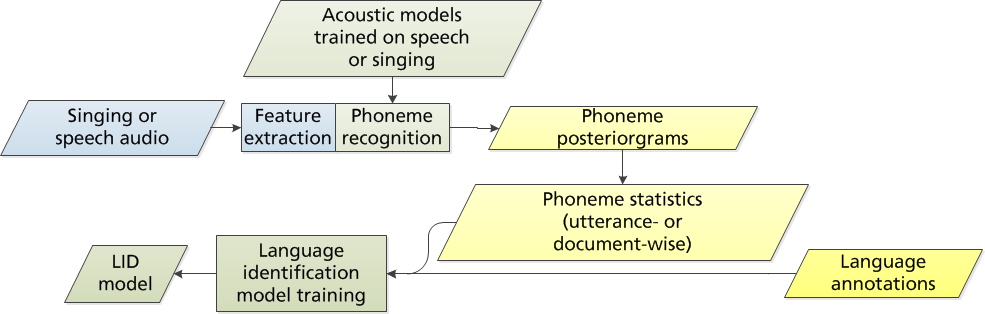
\includegraphics[width=1\textwidth]{images/process_lid_stats.png}
		\caption{Overview of the process for language identification using phoneme statistics.}
		\label{fig:lid_statistics_process}
	\end{center}
\end{figure*}

An overview of the approach is shown in figure \ref{fig:lid_statistics_process}. Posteriorgrams are generated on the test data sets \textit{YTAcap} and \textit{OGIMultilang} using the acoustic models trained on the \textit{TIMIT} speech data set and on the \textit{DAMP} singing data set as described in section \ref{sec:phonerec_acap}. To facilitate the following language identification, phoneme statistics are then calculated in two different ways:
\begin{description}
  \item[Document-wise statistics]{Mean and variances of the phoneme likelihoods over whole songs or sets of utterances of a single speaker are calculated. This results in just two feature vectors per document (one for the means, one for the variances).}
  \item[Utterance-wise statistics]{Means and variances of the phoneme likelihoods over each utterance are calculated (or, in the case of \textit{YTAcap}, over each song segment). For further training, the resulting vectors for each speaker/song (= document) are used as a combined feature matrix. As a result, no overlap of speakers/songs is possible between the training and test sets.}
\end{description}
Naturally, relatively long recordings are necessary to produce salient statistics. For this reason, the aggregation by speaker/song is done in both cases rather than treating each utterance separately. \\

Then, Support Vector Machine (SVM) models are trained on the calculated statistics in both variants with the three languages as annotations. Unknown song/speaker documents can then be subjected to the whole process and classified by language.\\
Again, all results are obtained using 5-fold cross-validation - i.e., SVMs are trained on 4/5 of each corpus, then the remaining 1/5 is classified with the model. This is done 5 times until each song/speaker document has been classified.

\subsection{Language identification using document-wise phoneme statistics}
In the first experiment, SVM classifiers are trained on the document-wise phoneme statistics, and classification is also performed on a document-wise basis (i.e., only one mean and one variance vector per document). The results are shown in figure \ref{fig:lid_statistics_res1}.\\
On the singing test set, results are worst when using acoustic models trained on \textit{TIMIT} at just $53\%$ accuracy, and become better when using the model trained on the ``songified'' \textit{TIMIT} variant \textit{TimitM} (see section \ref{sec:phonerec_songify}), or on the small selection of the singing training set \textit{DampBB\_small} at an accuracy of $59\%$ each. The best result of $63\%$ accuracy is achieved when the models are trained on the full singing data set.\\
Surprisingly, the results on the \textit{OGIMultilang} corpus also improve from $75\%$ with the \textit{TIMIT} models to $84\%$ using the \textit{DampB} models. Since \textit{TIMIT} is a very ``clean'' data set, training on the singing corpus might provide some more phonetic variety, acting as a sort of data augmentation. This could be especially important in this context where phonemes are recognized in three different languages.\\
On both corpora, there is no noticeable bias of the confusion matrix - i.e., the confusions are spread out evenly. This is particularly interesting when considering that the acoustic models were trained on English speech or singing only.
%\begin{figure}[h]
 %       \centering
  %      \begin{subfigure}[c]{0.25\textwidth}
  %              \includegraphics[width=\textwidth]%{figs/stat_acc.png}
   %             \caption{Accuracy}
   %             \label{fig:stat_acc}
  %      \end{subfigure}%
   %     ~ %add desired spacing between images, e. g. ~, \quad, \qquad, \hfill etc.
          %(or a blank line to force the subfigure onto a new line)
   %     \begin{subfigure}[c]{0.25\textwidth}
     %           \includegraphics[width=\textwidth]%{figs/stat_cavg.png}
   %             \caption{Average cost}
  %              \label{fig:stat_cavg}
 %       \end{subfigure}
 %       \caption{Results using document-wise phoneme statistics generated with various acoustic models.}\label{fig:res_stat}
%\end{figure}

\begin{figure*}
	\begin{center}
		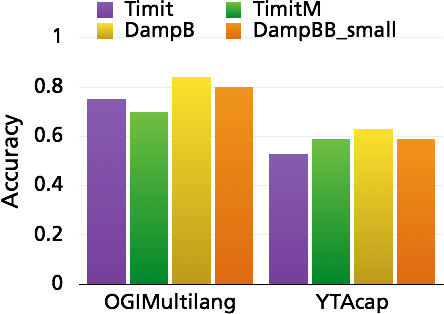
\includegraphics[width=.4\textwidth]{images/lid_statistics_res1.png}
		\caption{Results using document-wise phoneme statistics generated with various acoustic models.}
		\label{fig:lid_statistics_res1}
	\end{center}
\end{figure*}

\subsection{Language identification using utterance-wise phoneme statistics}
Next, language identification was performed with models trained on the statistics of each utterance contained in the document. The recognition process is still performed on the whole document. The results are reported in figure \ref{fig:lid_statistics_res2}.\\
Phoneme statistics may not be as representative when computed on shorter inputs, but they may provide more information for the backend model training when utilized as a combined feature matrix for a longer document. The results on singing improve slightly to $63\%$ accuracy with the acoustic model trained on the small singing corpus (\textit{DampBB\_small}) and decrease slightly for the \textit{DampB} model ($61\%$). However, on the speech corpus, the best result rises to $90\%$.
%why??
%\setlength{\belowcaptionskip}{-0.3cm}
%\begin{figure}[h]
 %       \centering
 %       \begin{subfigure}[c]{0.25\textwidth}
  %              \includegraphics[width=\textwidth]%{figs/stats_acc.png}
  %              \caption{Accuracy}
 %               \label{fig:stats_acc}
%        \end{subfigure}%
 %       ~ %add desired spacing between images, e. g. ~, \quad, \qquad, \hfill etc.
          %(or a blank line to force the subfigure onto a new line)
 %       \begin{subfigure}[c]{0.25\textwidth}
 %               \includegraphics[width=\textwidth]%{figs/stats_cavg.png}
 %               \caption{Average cost}
  %              \label{fig:stats_cavg}
  %      \end{subfigure}
  %      \caption{Results using utterance-wise phoneme statistics generated with various acoustic models.}\label{fig:res_stats}
%\end{figure}
%\setlength{\belowcaptionskip}{-0.1cm}
\begin{figure*}
	\begin{center}
		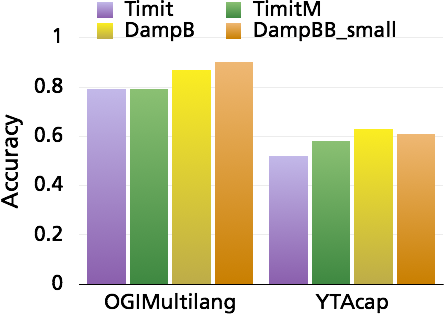
\includegraphics[width=.4\textwidth]{images/lid_statistics_res2.png}
		\caption{Results using utterance-wise phoneme statistics generated with various acoustic models.}
		\label{fig:lid_statistics_res2}
	\end{center}
\end{figure*}

\subsection{For comparison: Results for the i-vector approach}
For comparison, models from the previous approach were also trained on the same time scales. i-Vectors were calculated on the utterance- or the document-wise scale. This was done for PLP and MFCC features. The resulting i-vectors were then used to train SVMs in the same manner as in the previous experiments. (The difference here is that the models are already trained on the aggregated i-vectors, either with those for a whole document or with all i-vectors of the utterances constituting each document aggregated). The results are shown in figure \ref{fig:lid_statistics_res3}.\\
The best result obtained on \textit{YTAcap} data set is $68\%$ accuracy. This is only 5 percent points higher than the approach based on phoneme statistics, which is easier to implement. On the \textit{OGIMultilang} corpus, the difference is only 3 percent points ($93\%$). Of course, the advantage of the i-vector approach is that it can also be performed on much shorter inputs.\\

\begin{figure*}
	\begin{center}
		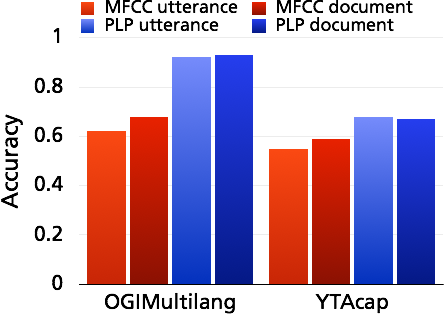
\includegraphics[width=.4\textwidth]{images/lid_statistics_res3.png}
		\caption{Results using utterance- and document-wise i-vectors calculated on PLP and MFCC features.}
		\label{fig:lid_statistics_res3}
	\end{center}
\end{figure*}
%\begin{figure}[h]
 %       \centering
%        \begin{subfigure}[c]{0.25\textwidth}
 %               \includegraphics[width=\textwidth]%{figs/ivec_acc.png}
  %              \caption{Accuracy}
   %             \label{fig:ivec_acc}
  %      \end{subfigure}%
  %      ~ %add desired spacing between images, e. g. ~, \quad, \qquad, \hfill etc.
          %(or a blank line to force the subfigure onto a new line)
 %       \begin{subfigure}[c]{0.25\textwidth}
 %               \includegraphics[width=\textwidth]%{figs/ivec_cavg.png}
 %               \caption{Average cost}
  %              \label{fig:ivec_cavg}
  %      \end{subfigure}
  %      \caption{Results using utterance- and document-wise i-vectors calculated on PLP and MFCC features.}\label{fig:res_ivec}
%\end{figure}

\section{Conclusion}\label{sec:lid_conclusion}
In this section, two approaches to singing language identification were presented: One based on i-vector processing of audio features, and one based on the computation of phoneme statistics from posteriorgrams. In both cases, machine learning models were trained on the resulting data.\\

In the first approach, PLP, MFCC, and SDC features are extracted from audio data, and then run through an i-vector extractor. The generated i-vectors are then used as inputs for MLP and SVM training. The basic idea behind the i-vector approach is the removal of language-independent components of the signal. This effectively reduces irrelevance to the language identification tasks and also reduces the amount of training data massively.\\
The smallest data set is the \textit{NIST2003LRE} corpus. No feature configuration achieves good results when using the MLP backend. In this case, the small size of the corpus may lead to overtraining. i-Vector processing only amplifies this problem by reducing the amount of data even further. The SVM backend, however, produces good results of up to 93\% for PLP features with i-vector extraction.\\
The \textit{OGIMultilang} corpus is a much bigger speech corpus. Training without i-vector extraction does not work well for any feature configuration. The best accuracy for this scenario was 68\%. Results of up to 83\% are achieved with i-vector processing. There does not seem to be a large difference between SVM and MLP training, with SVMs having just a slight advantage.\\
Language identification for singing was expected to be a harder task than for speech due to the factors described in section \ref{sec:sota_speechtosinging}. The results on the \textit{YTAcap} corpus turn out to be somewhat worse than those for the \textit{OGIMultilang} corpus, which is of similar size. Once again, i-vector extraction improves the results from 63\% to 73\%.\\
The same experiment is repeated with no speaker overlap between training and test sets. The results fall significantly, indicating speaker influence on the model training. In a third experiment, the results are aggregated into documents by each speaker, which again leads to improved results. The best accuracy on \textit{OGIMultilang} is $92\%$, while on \textit{YTAcap}, it is $69\%$. Both experiments demonstrate that useful results can be obtained when limiting the task, e.g. by training on a set of known speakers or recording conditions, or by analyzing documents of longer durations. Alternatively, a wider range of speakers in the training data could lead to models that generalize better.\\
Overall, i-vector extraction reduces irrelevance in the training data and thereby leads to a more effective training. As additional benefits, the training process itself is much faster and less memory is used due to its data reduction properties. Most of the state-of-the-art approaches are based on PPRLM, which requires phoneme-wise annotations and a highly complex recognition system, using both acoustic and language models. In this respect, this system is easier to implement and merely requires language annotations.\\

The second presented method is a completely new language identification approach for singing. It is based on the output of various acoustic models, from which statistics are generated and SVM models are trained. In contrast to similar approaches for speech, no voice tokenization is performed. Since phoneme recognition on singing is not always reliable, the statistics are calculated directly on the phoneme posteriorgrams, although this does not take any temporal information into account. The acoustic models are trained only on English-language material (speech and singing); it would be interesting to test this with multi-language training data. Due to the statistics-based nature of the approach, it is not suited for language identification of very short audio recordings.\\
The accuracy of the result for singing is somewhat worse than the results obtained with the i-vector based approach. However, this new approach is much easier to implement and the feature vectors are shorter. For many applications, such posteriors need to be extracted anyway and can efficiently be used for language identification when long observations are available. The best accuracy of $63\%$ is obtained with acoustic models trained on the \textit{DampB} singing corpus.\\
Interestingly, the best result on the \textit{OGIMultilang} speech corpus is also obtained with these acoustic models (and is only 3 percent points below the one obtained with the i-vector approach). This possibly happens because the singing corpora provide a wider range of phoneme articulations. It would be interesting to try out these acoustic models for other phoneme recognition tasks on speech where robustness to varied pronunciations is a concern.




\chapter{Sung keyword spotting experiments and results} \label{chap:kws}
Keyword spotting is another task for which the new acoustic models described in chapter \ref{chap:phonerec} were employed. A keyword-filler HMM algorithm was selected due to its independence on phoneme durations, which is a condition that cannot be fulfilled easily in singing. As described in section \ref{sec:tech_kwfhmm}, keyword-filler HMMs consist of two sub-HMMs: One to model the keyword and one to model everything else (=filler). The keyword HMM has a simple left-to-right topology with one state per keyword phoneme. The filler HMM is a fully connected loop of all phonemes. When the Viterbi path with the highest likelihood passes through the keyword HMM rather than the filler loop, the keyword is detected. Keyword detection was performed on whole songs, which is a realistic assumption for many practical applications. The \textit{ACAP} and \textit{DampTest} data sets were used for evaluation with the keyword set described in section \ref{sec:data_kws}. Song-wise $F_1$ measures were calculated for evaluation.

\section{Keyword spotting using keyword-filler HMMs}
\subsection{Comparison of acoustic models}
Phoneme posteriorgrams were generated with the various acoustic models described in section \ref{sec:phonerec_acap}. The results in terms of $F_1$ measure across the whole \textit{DampTest} sets are shown in figure \ref{fig:kws_exp1}. Figure \ref{fig:kws_exp1_acap} show the results of the same experiment on the small \textit{ACAP} data set.

Across all keywords, a document-wise $F_1$ measure of $0.35$ is obtained using the posteriorgrams generated with the \textit{TIMIT} model on the \textit{DampTest} data sets. This result is slightly higher for the \textit{TimitM} models trained on ``songified'' speech, and rises to $0.45$ using the model trained on the small \textit{DampBB\_small} singing data set. Surprisingly, the model trained on \textit{DampBB} is only slightly better than the much smaller one. Using the very big \textit{DampB} training data set, the $F_1$ measure reaches $0.47$. 

On the hand-annotated \textit{ACAP} test set, the difference is even more pronounced, rising from $0.29$ for the \textit{TIMIT} model to $0.5$ for \textit{DampB}. This might, again, be caused by the more accurate annotations or by the higher-quality singing. Additionally, the data set is much smaller with fewer occurrences of each keyword, which could emphasize both positive and negative tendencies in the detection.

%TODO: recall vs. precision -> �berleitung zu duration modeling


\begin{figure}
        \centering
        \begin{subfigure}[t]{0.4\textwidth}
		 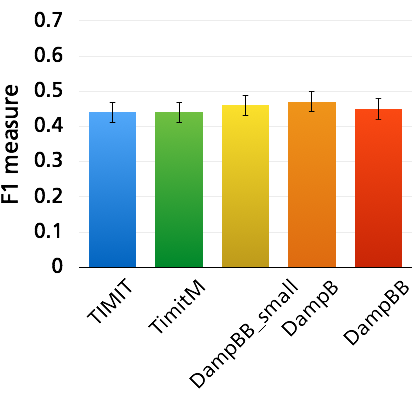
\includegraphics[width=\textwidth]{images/kws_exp1.png}
                \caption{$F_1$ measures for keyword spotting results on the \textit{DampTest} data sets.}
                \label{fig:kws_exp1}

        \end{subfigure}%
        \hfill
         %add desired spacing between images, e. g. ~, \quad, \qquad, \hfill etc.
          %(or a blank line to force the subfigure onto a new line)
        \begin{subfigure}[t]{0.4\textwidth}
                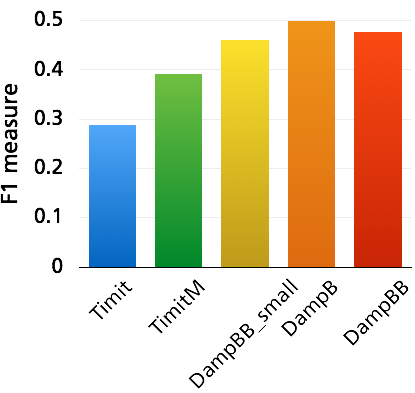
\includegraphics[width=\textwidth]{images/kws_exp1_acap.png}
                \caption{Keyword spotting results on the \textit{ACAP} data set.}
                \label{fig:kws_exp1a}
        \end{subfigure}
        \caption{$F_1$ measures for keyword spotting results using posteriorgrams generated with various acoustic models.}
          \end{figure}
%\vspace{-5px}

\subsection{Gender-specific acoustic models}
%TODO: ACAP??
Keyword spotting was also performed on the posteriorgrams generated with the gender-dependent models trained on \textit{DampF} and \textit{DampM} (also described in section \ref{sec:phonerec_acap}. The results are shown in figure \ref{fig:kws_exp2}.

In contrast to the phoneme recognition results from Experiment C, the gender-dependent models perform slightly better for keyword spotting than the mixed one of the same size, and almost as good as the one trained on much more data (\textit{DampB}). The $F_1$ measures for the female test set are  $0.48$ for the \textit{DampB} model, $0.45$ for the \textit{DampBB} model, and $0.46$ for the \textit{DampFB} model. For the male test set, they are $0.46$ and $0.45$ for the first two, and $0.46$ for the \textit{DampMB} model.



\subsection{Individual analysis of keyword results}
%TODO: ACAP??
Figure \ref{fig:kws_exp3} shows the individual $F_1$ measures for each keyword using the best model (\textit{DampB}), ordered by their occurrence in the \textit{DampTest} sets from high to low (i.e. number of songs which include the song). There appears to be a tendency for more frequent keywords to be detected more accurately. This happens because a high recall is often achievable, while the precision depends very much on the accuracy of the input posteriorgrams. The more frequent a keyword, the easier it also becomes to achieve a higher precision for it.

As shown in literature \cite{phdthesis:thambiratnam}, the detection accuracy also depends on the length of the keyword: Keywords with more phonemes are usually easier to detect. This might explain the relative peak for ``every", ``little", and ``always", in contrast to ``eyes" or ``world". Since keyword detection systems tend to perform better for longer words and most of the keywords only have 3 or 4 phonemes, this result is especially interesting.

One potential source of error are sequences of phonemes that overlap with keywords, but are not included in the calculation of the precision. Words spelled the same were included, but split phrases or other spellings were not (e.g. ``away" as part of ``castaway" would be counted, but ``a way" would not be counted as ``away"). This might artificially lower the results and could be an avenue for future improvement. Additionally, only one pronunciation for each keyword was provided, but there may be several possible.

\begin{figure}
 \begin{center}
                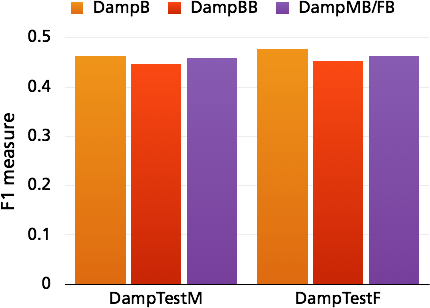
\includegraphics[width=0.5\textwidth]{images/kws_exp2.png}
                \caption{$F_1$ measures for keyword spotting results on the \textit{DampTestM} and \textit{DampTestF} data sets using mixed and gender-dependent models.}
                \label{fig:kws_exp2}
                 \end{center}
 \end{figure}

\begin{figure}
 \begin{center}
                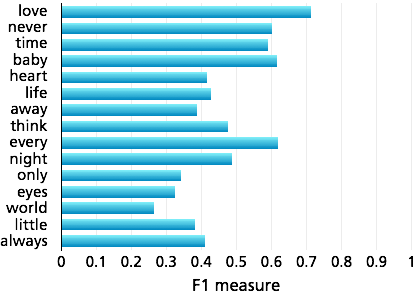
\includegraphics[width=0.5\textwidth]{images/kws_exp3.png}
                \caption{Individual $F_1$ measures for the results for each keyword, using the acoustic model trained on \textit{DampB}.}
                \label{fig:kws_exp3}
                 \end{center}
 \end{figure}
%\vspace{-5px}





\section{Keyword spotting using duration-informed keyword-filler HMMs}
As mentioned above, a high recall is easily achievable with the described approach, but the comparatively low precision decreases the over-all result. Therefore, using additional information to sort out false positives would be a helpful next step.\\
One such source of information are the durations of the detected phonemes. As shown in figure \ref{fig:phone_durations}, each phoneme in the \textit{TIMIT} speech database has a fairly fixed duration. In singing, the vowels' durations vary a lot, but the consonants' are still quite predictable. Standard HMMs do not impose any restrictions on the state durations, resulting in a geometric distribution which does not correspond to naturally observed phoneme durations. \\
As first described in \cite{ferguson}, introducing restrictions on state durations can improve the recognition results. In \cite{juang}, Juang et al. present two basic approaches for duration modeling in HMMs: Internal duration modeling and Post-processor duration modeling.\\

%todo: DOPPELT!!
In internal duration modeling, the durations are incorporated directly into the Viterbi alignment. This means that the Viterbi output will already be a state sequence that is optimal with regards to the a-priori phoneme duration knowledge. It is, however, computationally expensive. In previous experiments \cite{kruspe_kws2}, this approach did not produce better results than the much easier to implement post-processor duration modeling. Therefore, this section will focus on that approach.\\

When using post-processor duration modeling, knowledge about plausible phoneme durations is imposed on the result of the Viterbi alignment, the obtained state sequence. This is computationally cheap, but only results in a new likelihood score for the obtained sequence and does not provide better possible state sequences. The state sequence obtained from the Viterbi alignment is afterwards re-scored as described in section \ref{sec:tech_duration_modeling}, and all occurrences of the keyword with a score below a certain threshold are discarded.



%TODO: clean up
\section{Conclusion}\label{sec:kws_conclusion}
%insgesamt besser
%huge DampB set best, but 3% DampBB almost as good
% even v small DampBB_small better than Timit
% context does not help
% gender models slightly better for kws, not better for phone rec --> variability?
% results phonerec
% results kws - esp. interesting because short
%---auto alignment error source

In this chapter, an approach for keyword spotting using the new acoustic models trained on singing was described. This was done by extracting phoneme posteriorgrams generated with these new models from the audio and then running them through a keyword-filler approach to detect 15 keywords. The resulting $F_1$ measure rises from $0.35$ for the models trained on speech (\textit{TIMIT}) to $0.47$ for the new models. This result is especially interesting because most of the keywords have few phonemes.Gender-dependent models perform slightly better than mixed-gender models of the same size.\\
This approach was only tested with MFCC features. As preliminary experiments suggest \cite{kruspe_kws1}, other features like TRAP or PLP may work better on singing. So-called log-mel filterbank features have also been used successfully with DNNs \cite{hinton}. Another interesting factor is the size and configuration of the classifiers, of which only one was tested (after a small grid search to validate this choice). Other experiments also suggest that incorporating certain phoneme duration information into the recognition can improve the over-all results \cite{kruspe_kws2}.\\
As in the phoneme recognition experiments, there is only a slight amount of improvement between the acoustic model trained on all 6000 songs of the \textit{DAMP} data set and the one trained only on $4\%$ of this data. It would be interesting to find the exact point at which additional training data does not further improve the models. On the evaluation side, a keyword spotting approach that allows for pronunciation variants or sub-words may produce better results. Language modeling might also help to alleviate some of the errors made during phoneme recognition.\\
These models have not yet been applied to singing with background music, which would be interesting for practical applications. Since this would probably decrease the result when used on big, unlimited data sets, more specified systems would be more manageable, e.g. for specific music styles, sets of songs, keywords, or specialized applications. Searching for whole phrases instead of short keywords could also make the results better usable in practice.\\
As shown in \cite{mesaros_alignment} and \cite{goto_alignment} and in the next chapter, alignment of textual lyrics and singing already works well. A combined approach that also employs textual information could be very practical.


\chapter{Lyrics Retrieval and Alignment} \label{chap:retrieval_alignment}

Lyrics retrieval and alignment are related tasks: The retrieval task can be interpreted as an alignment of all possible lyrics sequences to the query audio, and a subsequent selection of the best-matching result. This is done in all described algorithms.\\
As a starting point, a traditional HMM-based algorithm for Forced Alignment was tested. Building on top of the posteriorgrams extracted with the new acoustic models as described in chapter \ref{chap:phonerec}, a new algorithm using Dynamic Time Warping (DTW) was developed and evaluated for both alignment and retrieval. Next, another processing step for explicitly extracting phonemes from the posteriorgrams was included; the resulting method was also tested for both alignment and retrieval. All three mentioned algorithms were entered into the 2017 \textit{MIREX} challenge for lyrics-to-audio alignment, in which the algorithms were tested on Hansen's dataset, both in the singing-only and polyphonic conditions (\textit{ACAP} and \textit{ACAP\_Poly}, see sections \ref{subsec:data_hansen} and \ref{subsec:data_hansen_polyphonic}), and on Mauch's alignment data set (\textit{Mauch}, see section \ref{subsec:data_mauch_alignment}). The results can be viewed on \url{http://www.music-ir.org/mirex/wiki/2017:Automatic_Lyrics-to-Audio_Alignment_Results} (last checked: ???).\\
Finally, a practical application for lyrics alignment is presented: Automatic expletive detection in rap songs.


\section{HMM-based lyrics-to-audio alignment}\label{sec:ret_hmm}
For this algorithm, monophone Hidden Markov Models were trained on the \textit{TIMIT} speech data using the HTK framework \cite{htk}. Then, Viterbi alignment was run to align the phonemes to the singing audio. These are the same models used to align lyrics to the \textit{DAMP} audio data to generate the training data set described in section \ref{sec:phonerec_acap}. The results in the \textit{MIREX} challenge are shown in figure \ref{fig:results_align_hmm}. The detailed results for all tested songs are given in appendix \ref{app:mirex_htk}.\\
On the unaccompanied data set, the mean error is $5.11s$, while the median error is $0.67s$. The large difference comes about because one of the tested songs (``Clocks'') produced high error values in every approach. Considering only the other songs, the highest error is $1.45s$, and all others are lower than $1s$. This is a good result, especially considering that the approach is relatively simple and trained on speech data only. A manual check suggests that the results are usable in practice.\\
On the accompanied version of the same data set, the average error is $13.96s$ and the median error is $7.64$. On the \textit{Mauch} data set, the mean error is at $17.7s$ and the median error is at $10.14s$. Once again, the error varies widely across the songs. As expected, the result is worse since no measures were taken make the approach robust to background music. Interestingly, other submitted approaches that employ sources separation did not fare much better on this data set either, suggesting that the core algorithm may be better. It would be interesting to see results for the HMM-based algorithm on polyphonic music with a source separation step (or at least a vocal activity detection step) included.\\
%TODO erkl�ren
\begin{figure}
 \begin{center}
                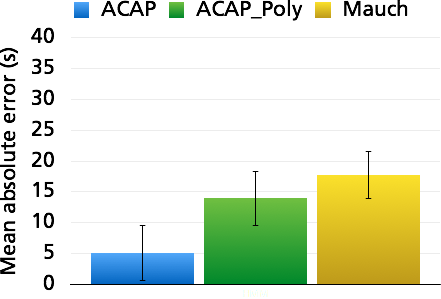
\includegraphics[width=0.5\textwidth]{images/res_align_hmm.png}
               \caption{\textit{MIREX} results on all three data sets using the HMM-based approach.}
                \label{fig:results_align_hmm}
                 \end{center}
 \end{figure}


\section{Posteriorgram-based retrieval and alignment}\label{sec:ret_post}

\begin{figure}
 \begin{center}
                \includegraphics[width=0.8\textwidth]{images/retrieval_dtw_process.png}
                \caption{Overview of the DTW-based lyrics alignment and retrieval method.}
                \label{fig:retrieval_dtw_process}
                 \end{center}
 \end{figure}

A new approach is based on the posteriorgrams generated with the DNN acoustic models described in section \ref{sec:phonerec_acap}; an overview is illustrated in figure \ref{fig:retrieval_dtw_process}. In order to align lyrics to these posteriorgrams, binary templates are generated from the text lyrics on the phoneme scale. These can be seen as oracle posteriorgrams, but do not include any timing information.\\
Between this template and the query posteriogram, a similarity matrix is calculated using the cosine distance. On the resulting matrix, Dynamic Time Warping (DTW) is then performed using the implementation from \cite{ellis_dtw} to obtain the alignment. An example is shown in figure \ref{fig:retrieval_dtw}.\\
Two optimizations were made to the algorithm. The first one was a sub-sampling of the phoneme posteriorgrams by the factor 10 (specifically, the mean for 10 consecutive frames was calculated). This increased the speed of the DTW for the individual comparisons and also produced better results. Longer windows were also tested, but this had a negative impact on the result.\\
Secondly, squaring the posteriorgrams before the similarity calculation produced slightly better results. This makes the posteriorgrams more similar to the binary lyrics templates used for comparison. Binarizing them was also tested, but this emphasized phoneme recognition errors too much.\\

In the retrieval case, the binary templates are generated for all possible lyrics in the database, and the DTW calculation is performed for each of them with the query posteriorgram. The DTW cost is used as the measure to obtain the best-matching lyrics. Since the phoneme durations in the actual recording and the lyrics templates have different lengths, the length of the warping path should not be a detrimental factor in cost calculation. 
Therefore, the accumulative cost of the best path is divided by the path length and then retained as a score for each possible lyrics document. In the end, the lyrics document with the lowest cost is chosen as a match (or, in some experiments, the N documents with the lowest costs).\\
As an additional experiment, both the textual lyrics corpus and the sung inputs were split into smaller segments roughly corresponding to one line in the lyrics each (around 12,000 lines). The retrieval process was then repeated for these inputs. This allowed an evaluation as to how well lyrics could be retrieved from just one single sung line of the song. (Sub-sequence DTW could also be used for this task instead of splitting both corpora.)\\


\begin{figure}
	\centering
	\begin{subfigure}[t]{0.5\textwidth}
		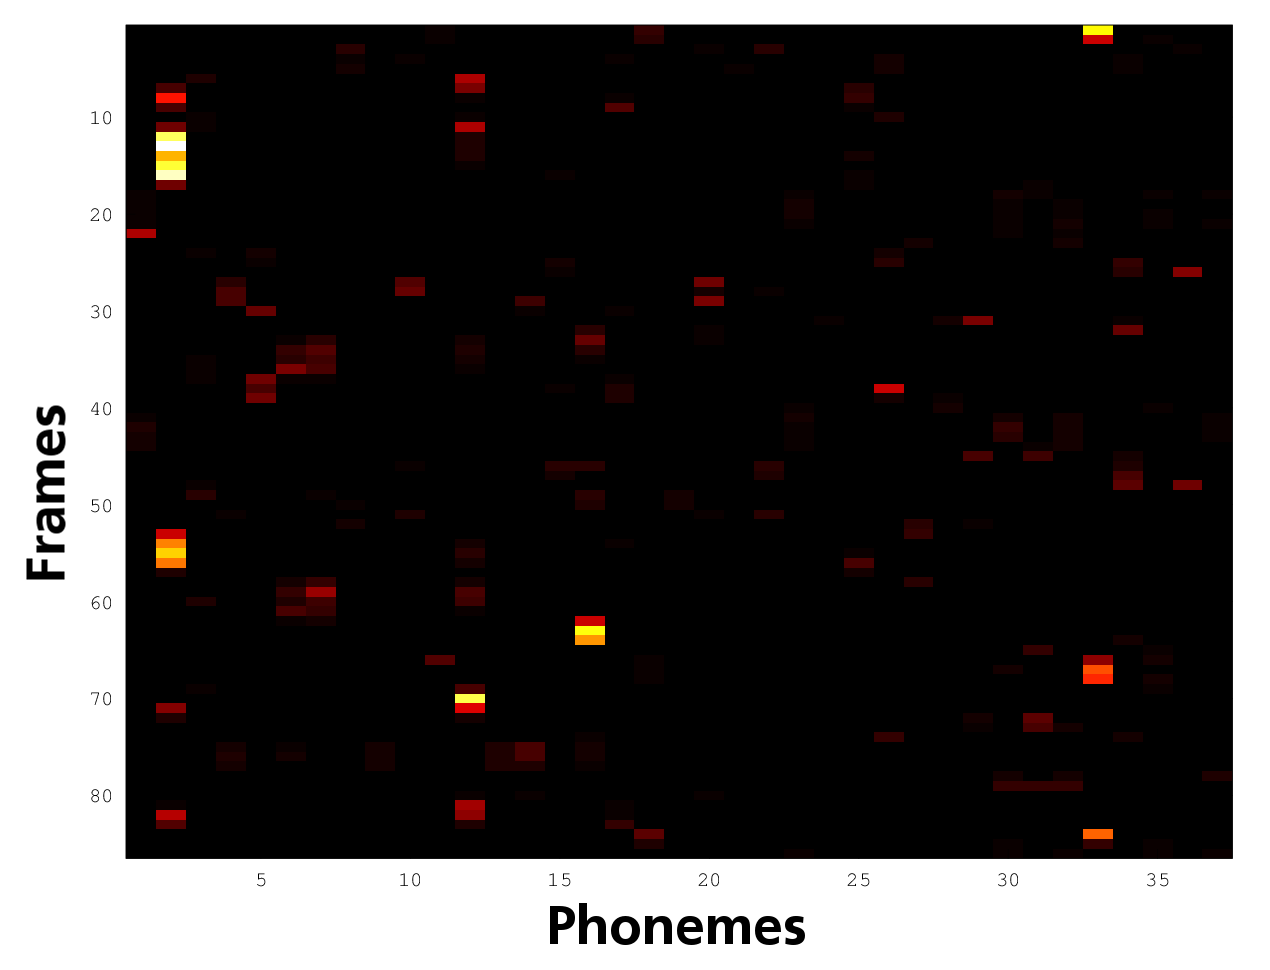
\includegraphics[width=\textwidth]{images/retrieval_posts.png}
		\caption{Phoneme posteriorgram}
		
	\end{subfigure}%
	%add desired spacing between images, e. g. ~, \quad, \qquad, \hfill etc.
	%(or a blank line to force the subfigure onto a new line)
	\begin{subfigure}[t]{0.5\textwidth}
		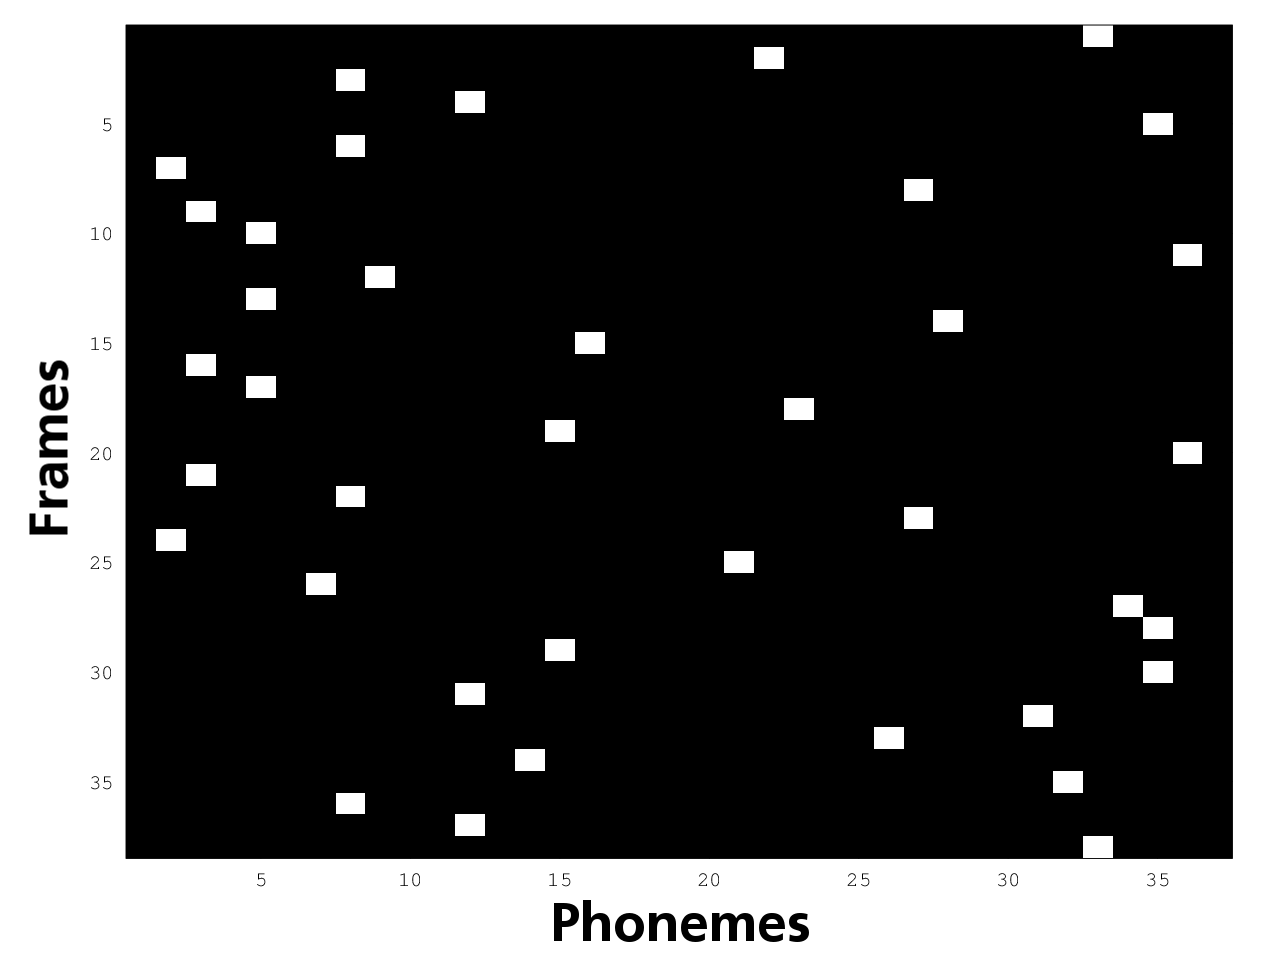
\includegraphics[width=\textwidth]{images/retrieval_template.png}
		\caption{Phoneme template}
	\end{subfigure}

	\begin{subfigure}[t]{0.5\textwidth}
		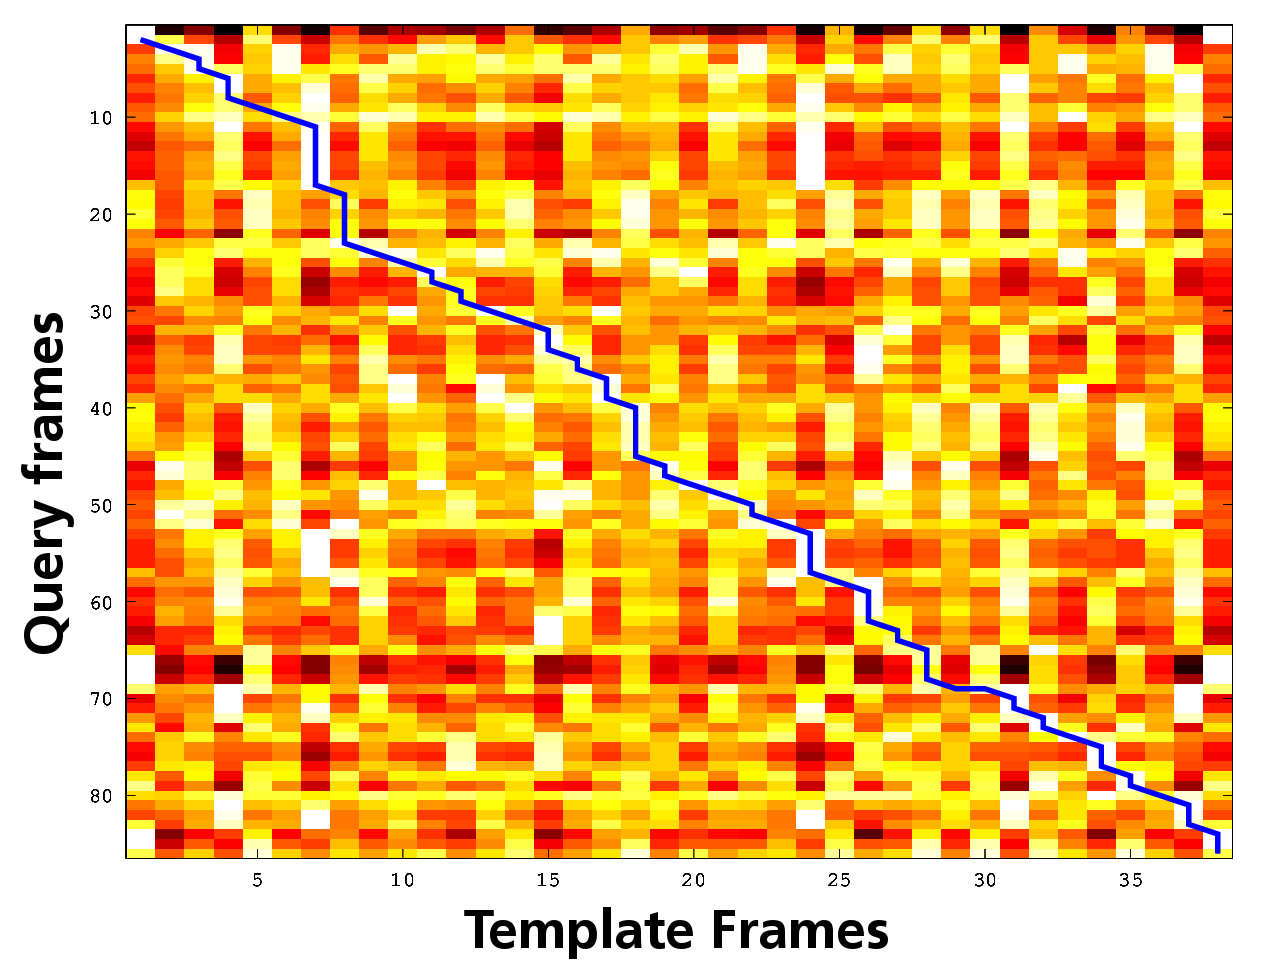
\includegraphics[width=\textwidth]{images/retrieval_similarity.png}
		\caption{Similarity matrix with cheapest path (blue)}
	\end{subfigure}
	\caption{Example of a similarity calculation: Phoneme posteriorgrams are calculated for the audio recordings \textbf{(a)}. Phoneme templates are generated for the textual lyrics \textbf{(b)}. Then, a similarity matrix is calculated using the cosine distance between the two, and DTW is performed on it \textbf{(c)}. The accumulated cost divided by the path length is the similarity measure.}\label{fig:retrieval_dtw}
\end{figure}

\subsection{Alignment experiments}
The results for this approach in the \textit{MIREX} challenge are displayed in figure \ref{fig:results_align_dtw}, with the detailed results given in appendix \ref{app:mirex_dtw}. Overall, errors are much higher than with the HMM-based approach: The mean error is $9.77s$ for the \textit{ACAP} data set, $27.94s$ on the \textit{ACAP\_Poly} data set, and $22.23s$ on the \textit{Mauch} data set. This presumably happens because in contrast to the HMM approach, the algorithm does not have any information about phoneme priors and transition probabilities, neither implicitly nor explicitly. DTW on the posteriorgram is a relatively rudimentary method for performing alignments. Nevertheless, a manual check of the results suggests that the algorithm is still able to produce usable results in many cases, with many song-wise results for the \textit{ACAP} data set still below $1s$. In particular, it works acceptably when the posteriorgram is not too noisy. This is also corroborated by the retrieval results for unaccompanied queries presented in the following.\\
As a future step, incorporating prior phoneme information (e.g. in the form of DNN-HMMs) could serve to mitigate some of the noise in the posteriorgram caused by model inaccuracies or by background music.

\begin{figure}
 \begin{center}
                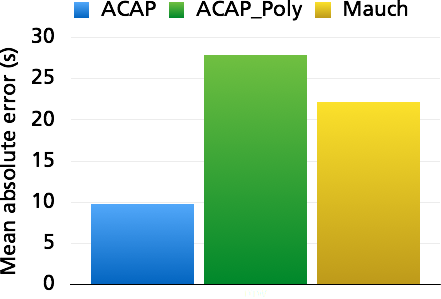
\includegraphics[width=0.8\textwidth]{images/res_align_dtw.png}
               \caption{\textit{MIREX} results on all three data sets using the DTW-based approach.}
                \label{fig:results_align_dtw}
                 \end{center}
 \end{figure}



\subsection{Retrieval experiments on whole song inputs}
In the first experiment, similarity measures were calculated between the lyrics and recordings of whole songs using the described process. This was tested with phoneme posteriorgrams obtained with all five acoustic models on the female and the male test sets (\textit{DampTestF} and \textit{DampTestM}). The accuracy was then calculated on the 1-, 3-, and 10-best results for each song (i.e., how many lyrics are correctly detected when taking into account the 1, 3, and 10 lowest distances?). The results on the female test set are shown in figure \ref{fig:retrieval_dtwres_testF}, the ones for the male test set in figure \ref{fig:retrieval_dtwres_testM}.

\begin{figure}
       \centering
        \begin{subfigure}[b]{0.4\textwidth}
	    \includegraphics[width=\textwidth]{images/retrieval_dtwres_testF.png}
                \caption{DampTestF}
                \label{fig:retrieval_dtwres_testF}
        \end{subfigure}%
         %add desired spacing between images, e. g. ~, \quad, \qquad, \hfill etc.
          %(or a blank line to force the subfigure onto a new line)
         \vspace{10px}
        \begin{subfigure}[b]{0.4\textwidth}
	  \includegraphics[width=\textwidth]{images/retrieval_dtwres_testM.png}
                \caption{DampTestM}
                \label{fig:retrieval_dtwres_testM}
        \end{subfigure}

        \caption{Accuracies of the results for lyrics detection on the whole song for the \textit{DampTest} sets using the DTW-based approach with five different acoustic models, and evaluated on the 1-, 3-, and 10-best results.}\label{fig:retrieval_dtwres}
\end{figure}

 These results show that phoneme posteriorgrams obtained with models trained on speech data (\textit{TIMIT}) generally produce the lowest results in lyrics retrieval. The difference between the two test sets is especially interesting here: On the male test set, the accuracy for the single best result is $58\%$, while on the female set it is only $39\%$. Previous experiments showed that the phoneme recognition itself performs somewhat worse for female singing inputs. This effect is compounded in these lyrics retrieval results. This may happen because the frequency range of female singing is even further removed from that of speech than the frequency range of male singing is \cite{sundberg}. Even female speech is often performed at the lower end of the female singing frequency range. The frequency range of male singing is better covered when training models on speech recordings (especially when speech recordings of both genders are used).\\
 This effect is still visible for the \textit{TimitM} models, which is the variant of \textit{Timit} that was artificially made more ``song-like''. However, the pitch range was not expanded too far in order to keep the sound natural.\\
The results improve massively when acoustic models trained on any of the \textit{DAMP} singing corpora are used. The difference between the male and female results disappears, which supports the idea that the female pitch range was not covered well by the models trained on speech. Using the models trained on the smallest singing data set (\textit{DampBB\_small}), which is slightly smaller than \textit{Timit}, the results increase to $81\%$ and $83\%$ for the single best result on the female and the male test set respectively. With the models trained on the \textit{DampBB} corpus, which is about twice as big, they increase slightly more to $85\%$ on the female test set. Gender-specific models of the same size do not improve the result in this case.\\
Finally, the results obtained with the acoustic models trained on the largest singing corpus (\textit{DampB}) provide the very best results at accuracies of $87\%$ and $85\%$.\\
For some applications, working with the best N instead of just the very best result could be useful (e.g. for presenting a selection of possible lyrics to a user). When the best 3 results can be taken into account, the accuracies on the best posteriorgrams rise to $89\%$ and $88\%$ on the female and male test sets respectively. When the best 10 results are used, they reach $92\%$ and $89\%$.

\subsection{Lyrics retrieval experiments on line-wise inputs}
\vspace{-2px}
In the second retrieval experiment, the same process was performed on single lines of sung lyrics as inputs (usually a few seconds in duration). Costs were then calculated between the posteriorgrams of these recordings and all 12,000 available lines of lyrics. Lines with fewer than 10 phonemes were not taken into account.\\
Then, evaluation was performed as to whether a line from the correct song was retrieved in the N-best results. In this way, confusions between repetitions of a line in the same song did not have an impact on the result. However, repetitions of lyrical lines across multiple songs are a possible source of confusion. The results for the female test set are shown in figure \ref{fig:retrieval_dtwres_testF_line}, the ones for the male test set in figure \ref{fig:retrieval_dtwres_testM_line}.
\begin{figure}
        \centering
        \begin{subfigure}[b]{0.4\textwidth}
	    \includegraphics[width=\textwidth]{images/retrieval_dtwres_testF_line.png}
                \caption{DampTestF}
                \label{fig:retrieval_dtwres_testF_line}
        \end{subfigure}%
        %add desired spacing between images, e. g. ~, \quad, \qquad, \hfill etc.
          %(or a blank line to force the subfigure onto a new line)
          \vspace{10px}
       \begin{subfigure}[b]{0.4\textwidth}
	  \includegraphics[width=\textwidth]{images/retrieval_dtwres_testM_line.png}
                \caption{DampTestM}
                \label{fig:retrieval_dtwres_testM_line}
       \end{subfigure}
        \caption{Accuracies of the results for lyrics detection on separate lines of sung lyrics for the \textit{DampTest} sets using the DTW-based approach with five different acoustic models, and evaluated on the 1-, 3-, 10-, 50-, and 100-best results.}\label{fig:retrieval_dtwres_line}
\end{figure}

Again, a difference between both test sets is visible when generating posteriograms with the \textit{TIMIT} models. The accuracy on the best result is $14\%$ for the male test set, but just $7\%$ for the female test.\\
The results for the \textit{DAMP} models show the same basic tendencies as before, although naturally much lower. For the single best result, the accuracies when using the \textit{DampB} model are $38\%$ and $36\%$ on the female and male test sets respectively. For this task, gender-dependent models produce slightly higher results than the mixed-gender ones of the same size.\\



\section{Phoneme-based retrieval and alignment}
Next, another step was introduced to improve the previous approach and make it more flexible. This step serves to compress the posteriorgrams down to a plausible sequence of phonemes, which can then be used to search directly on a textual lyrics database. Text comparison is much cheaper than the previous comparison strategy, and enables quick expansion of the lyrics database.\\
In parallel, the lyrics database is prepared by converting it into phoneme sequences as described in section \ref{}. The key algorithms are (a) how to generate plausible phoneme sequences from the posteriorgrams, and (b) how to compare these against the sequences in the database. These parts will be described in more detail in the following. An overview is given in figure \ref{fig:retrieval_phone_overview}.

%TODO: phoneme seqs erkl�ren
\begin{figure}
 \begin{center}
                \includegraphics[width=.8\textwidth]{images/retrieval_phone_overview.png}
                \caption{Overview of the phoneme-based lyrics retrieval process.}
                \label{fig:retrieval_phone_overview}
                 \end{center}
 \end{figure}

\vspace{-5pt}
\paragraph{Symbolic mapping} \label{par:symbolic_mapping}
As described before, starting from the sung recording used as a query, MFCC features are extracted and run through the acoustic model trained on singing to recognize the contained phonemes. This produces a phoneme posteriorgram, such as the one shown in figure \ref{fig:posteriorgram}; i.e., probabilities of each phone over each time frame. These probabilities contain some noise, both due to inaccuracies in the model and due to ambiguities or actual noise in the performance.\\ %Why not HMMSs??
The following steps are undertaken to obtain a plausible phoneme sequence from the posteriorgram:
\begin{description}
	\item[Smoothing] First, the posteriorgram is smoothed along the time axis with a window of length 3 in order to remove small blips in the phoneme probabilities. 
	\item[Maximum selection and grouping] Then, the maximum bin (i.e. phoneme) per frame is selected, and consecutive results are grouped. An example is given in figure \ref{fig:retrieval_phone_block1}.
	\item[Filtering by probability and duration] These results can then be pre-filtered to discard those that are too short or to improbable. This is done with different parameterizations for vowels and consonants since vowels are usually longer in duration. This yields a first sequence of phonemes, each with duration and sum probability information, which is usually too long and noisy. In particular, a lot of fluctuations between similar phonemes occur. %; an example is shown in figure \ref{fig:}.
	\item[Grouping by blocks and filtering through confusion matrix] This problem is solved by first grouping the detected phonemes into blocks, in this case vowel and consonant blocks (shown in figure \ref{fig:block2}). Then, a decision needs to be made as to which elements of these blocks are the ``true'' phonemes and which ones are noise. This is done by taking each phoneme's probability as well as the confusion between phonemes into account. The confusion is calculated in advance by running the classifier on an annotated test set; the result covers both the confusion by inaccuracies in the classifier as well as perceptual or performance-based confusions (e.g. transforming a long \textit{[ay]} sound into \textit{[aa - ay - iy]} during singing). An example is shown in figure \ref{fig:retrieval_phone_confusion}. The product of the probabilities and the confusions are calculated for the highest combinations up to a certain threshold, and all other detected phonemes are discarded. This results in a shorter, more plausible phoneme sequence (figure \ref{fig:retrieval_phone_block3}).% such as the example shown in figure \ref{fig:}.
\end{description}
%listing?

  \begin{figure}

	\centering
	\begin{subfigure}[t]{0.4\textwidth}
		\includegraphics[width=.8\textwidth]{images/retrieval_phone_block1.png}
		\caption{Original phoneme sequence}\label{fig:retrieval_phone_block1}
	\end{subfigure}%
	\begin{subfigure}[t]{0.4\textwidth}
		\includegraphics[width=.8\textwidth]{images/retrieval_phone_block2.png}
		\caption{Grouped into blocks (with probabilities in italics)}\label{fig:retrieval_phone_block2}
	\end{subfigure}
	\begin{subfigure}[t]{0.4\textwidth}
		\includegraphics[width=.8\textwidth]{images/retrieval_phone_block3.png}
		\caption{Filtered result}\label{fig:retrieval_phone_block3}
	\end{subfigure}

	\caption{Example of the block grouping of the phoneme sequence and subsequent filtering by probabilities and confusions.}\label{fig:retrieval_phone_blocking}
\end{figure}

\begin{figure}
	\begin{center}
		\includegraphics[width=.8\textwidth]{images/retrieval_phone_confusion.png}
		\caption{Example of a confusion matrix for an acoustic model. (Note that \textit{[pau]} confusions are set to 0).}
		\label{fig:retrieval_phone_confusion}
	\end{center}
\end{figure}

\begin{table}[h!tp]
\footnotesize
\begin{center}
\begin{tabular}{|c||c|c|c||c|c|c||c|c|c|}
\hline
 & \multicolumn{3}{|c|}{Female} & \multicolumn{3}{|c|}{Male} & \multicolumn{3}{|c|}{Author} \\
 & Top1 & Top3 & Top10 & Top1 & Top3 & Top10 & Top1 & Top3 & Top10 \\
\hline \hline
Baseline & .25 & .25 & .35 & .1 & .1 & .2 & .1 &.23 &.36 \\
\hline
Posteriorgram smoothing & .65 & .7 & .90 & .5 & .65 &.65 &.61 &.67 &.76 \\
\hline
Filtering blocks by probabilities and confusions & .8 & .85 &.96 & .75 &.8 &.85 &.74 &.78 &.82 \\
\hline
Substitution weights & .9 &.95 &.95 &.65 &.8 &.9 &.76 &.78 &.83 \\
\hline
Substitution + Insertion weights & 1 & 1 & 1 & .75 & .85 &.9 &.81 &.84 &.9 \\
\hline
\end{tabular}
\end{center}
\caption{Results of the retrieval algorithm for three test data sets with various improvement steps.}
\label{tab:results}
\end{table}%

\vspace{-5pt}
\paragraph{Distance calculation} \label{par:lev_distance}
Then, the distances between the extracted phoneme sequence and the ones provided in the lyrics database are calculated.\\
First, an optional step to speed up the process is introduced. Each sequence's number of vowels is counted in advance, and the same is done for the query sequence. Then, only sequences with roughly the same amount of vowels are compared (with some tolerance). This slightly decreases accuracies, but drastically speeds up the calculation time.\\
The similarity calculation itself is implemented with a modified Levenshtein distance. Again, the classifier's confusion between phonemes is taken into account. These confusions are used as the Levenshtein weights for substitutions. Surprisingly, using them for insertion weights improves the results as well. This probably happens because of the effect described above: A singer will in many cases vocalize an phoneme as multiple different ones, particularly for vowels with long durations. This will result in an insertion in the detected phoneme sequence, which is not necessarily a ``wrong'' classification by the acoustic model, but does not correspond to the expected sequence for this line of lyrics. For this reason, such insertions should not be harshly penalized. For deletions, the weight is set to $.5$ to balance out the lower insertion and substitution weights.



\subsection{Alignment experiments}
\textit{MIREX} results for this approach are shown in figure \ref{fig:results_align_phone}; the detailed results can be found in appendix \ref{app:mirex_phone}. Over-all, this approach produces much lower error values than the other two, and was in fact the winning algorithm in the competition. This confirms that the phoneme detection strategy is a feasible alternative to the HMM-based approach. On the \textit{ACAP} data set, the mean error is at $2.87s$ and the median is $0.26s$. On \textit{ACAP\_Poly}, these values are $7.34s$ and $4.55s$ respectively, and on \textit{Mauch}, they are $9.03s$ and $7.52s$. Once again, the results are much higher on polyphonic data than on unaccompanied singing, for which the models were trained. However, the error is still lower than with the submitted methods that include source separation. Therefore, future experiments that also employ pre-processing of this kind would be very interesting. Looking at the song-wise results, songs with heavier and noisier accompaniment generally receive higher errors than others.
\begin{figure}
 \begin{center}
                \includegraphics[width=0.5\textwidth]{images/res_align_phone.png}
               \caption{\textit{MIREX} results on all three data sets using the phoneme-based approach.}
                \label{fig:results_align_phone}
                 \end{center}
 \end{figure}
 

\subsection{Retrieval experiments: Calibration}
For calibrating the algorithm's parameters quickly, two smaller data sets were used: \textit{DampRetrieval}, which consists of 20 female and 20 male hand-selected sung segments with clear pronunciation and good audio quality, and \textit{AuthorRetrieval}, which consists of 90 small performances of phrases in the \textit{DAMP} data set by the author. Both are described in sections \ref{subsec:data_damp} and \ref{subsec:data_retrieval}. This was done to ensure that the results were not influenced by flaws in the data set (such as unclear or erroneous pronunciation or bad quality). Lyrics can still come from the whole \textit{DAMP} lyrics set, resulting in 12,000 lines of lyrics from 300 songs.\\
Table \ref{tab:results_retrieval_phone} shows an overview over the experimental results. Retrieval rates are reported for the Top 1 result (i.e. the one with the lowest Levenshtein distance), the Top 3, and the Top 10 results. Queries were allowed to be one to three consecutive lines of songs, increasing the number of ``virtual'' database entries to around 36,000 (12,000 lines as 1-, 2-, and 3-grams). It should be noted that a result counts as correct when the correct song (out of 300) was detected; this was done as a simplification because the same line of lyrics is often repeated in songs. For possible applications, users are most probably interested in obtaining the correct full song lyrics, rather than a specific line. Picking random results would therefore result in a retrieval rate of $.003$.\\
The various improvement steps of the algorithm were tested as follows:
\begin{description}
\item[Baseline] This is the most straightforward approach: Directly pick the phonemes with the highest probabilities for each frame from the posteriorgram, group them by consecutive phonemes, and use the result of that for searching the lyrics database with a standard Levenshtein implementation. This results in retrieval rates of $.25$, $.1$, and $.23$ for the Female, Male, and Author test sets respectively.
\item[Posteriorgram smoothing] This is the same as the baseline approach, but the posteriorgram is smoothed along the time axis as described in paragraph \ref{par:symbolic_mapping}. This already improves the result by around $.4$ for each test set.
\item[Filtering blocks by probabilities and confusions] This includes the last step described in paragraph \ref{par:symbolic_mapping}. The result is improved further by $.13$ to $.25$.
\item[Substitution and insertion weights] Finally, the modified Levenshtein distance as described in paragraph \ref{par:lev_distance} is calculated. When using the confusion weights for phoneme substitutions only, the result increases further, and even more so when they are also used for the insertion weights. The final Top 1 retrieval rates are $1$, $.75$, and $.81$ for the three test sets respectively.
\end{description}

\subsection{Retrieval experiments: Full data set}
The full algorithm was then also run on the full \textit{DampTest} data sets in the same way as the DTW-based approach.


\begin{figure}
	\centering
	\begin{subfigure}[b]{0.4\textwidth}
		\includegraphics[width=\textwidth]{images/retrieval_levres_testF.png}
		\caption{DampTestF}
		\label{fig:retrieval_levres_testF}
	\end{subfigure}%
	%add desired spacing between images, e. g. ~, \quad, \qquad, \hfill etc.
	%(or a blank line to force the subfigure onto a new line)
	\vspace{10px}
	\begin{subfigure}[b]{0.4\textwidth}
		\includegraphics[width=\textwidth]{images/retrieval_levres_testM.png}
		\caption{DampTestM}
		\label{fig:retrieval_levres_testM}
	\end{subfigure}
	
	\caption{Accuracies of the results for lyrics detection on the whole song for the \textit{DampTest} sets using the phoneme-based approach with five different acoustic models, and evaluated on the 1-, 3-, and 10-best results.}\label{fig:retrieval_levres}
\end{figure}

\begin{figure}
	\centering
	\begin{subfigure}[b]{0.4\textwidth}
		\includegraphics[width=\textwidth]{images/retrieval_levres_testF_line.png}
		\caption{DampTestF}
		\label{fig:retrieval_levres_testF_line}
	\end{subfigure}%
	%add desired spacing between images, e. g. ~, \quad, \qquad, \hfill etc.
	%(or a blank line to force the subfigure onto a new line)
	\vspace{10px}
	\begin{subfigure}[b]{0.4\textwidth}
		\includegraphics[width=\textwidth]{images/retrieval_levres_testM_line.png}
		\caption{DampTestM}
		\label{fig:retrieval_levres_testM_line}
	\end{subfigure}
	\caption{Accuracies of the results for lyrics detection on separate lines of sung lyrics for the \textit{DampTest} sets using the phoneme-based approach with five different acoustic models, and evaluated on the 1-, 3-, 10-, 50-, and 100-best results.}\label{fig:retrieval_levres_line}
\end{figure}


\section{Application: Expletive detection}

Lots of song lyrics contain expletives. There are many scenarios in which it is necessary to know when these words occur, e.g. for airplay and for the protection of minors. In the case of airplay, they are commonly ``bleeped" or acoustically removed. The alignment strategies described previously are employed for the practical scenario of finding such expletives automatically.\\
The test data set is the one compiled by Queen Mary University, described in section \ref{subsec:data_qmul}.\\

A direct keyword spotting approach was also considered, but this did not generate sufficient results since most of the expletives only consist of 2 or 3 phonemes. Keyword spotting becomes notoriously hard for such short keywords as described in chapter \ref{chap:kws}.\\
Since textual lyrics are usually easily available on the internet, a new approach utilizing those was developed:
\begin{enumerate}
\item Automatically align textual lyrics to audio (as described above)
\item Search for pre-defined expletives in the result
\item If necessary, remove those expletives. A stereo subtraction approach was used, which works adequately for this case since the removed timespans are short. Alternatively, keywords can be masked with a bleep or similar.
\end{enumerate}
The data flow is shown in figure \ref{fig:expletive_dataflow}.
\begin{figure}
\begin{center}
                \includegraphics[width=0.6\textwidth]{images/expletive_approach.png}
                \caption{Data flow in the expletive detection approach.}
                \label{fig:expletive_dataflow}
                 \end{center}
 \end{figure}

The alignment was performed using the HMM-based alignment described in section \ref{sec:ret_hmm}, and the DTW alignment from section \ref{sec:ret_post} using the DNN acoustic models trained on \textit{TIMIT} and on \textit{DampB}. Accuracy was then calculated by evaluating how many of the annotated expletives were recognized at their correct timestamps (with various tolerances). The results are shown in figure \ref{fig:expletive_results}.
\begin{figure}
 \begin{center}
                \includegraphics[width=0.6\textwidth]{images/expletive_results.png}
               \caption{Results for the expletive detection approach at various tolerances.}
                \label{fig:expletive_results}
                 \end{center}
 \end{figure}
 %analyze?

In this small practical example, only two alignment strategies were tested, but there are others that could provide better results. Whenever the alignment failed, it was mostly due to solo instruments. In order to remedy this, vocal detection (and possibly source separation) could be employed prior to alignment. Additionally, a more sophisticated removal approach could be implemented to remove the expletives.\\
Lyrics collected from the internet are often incorrect, e.g. because repetitions are not spelled out, because of spelling errors, or because they refer to different versions of a song. This approach could be expanded to allow for some flexibility in this respect. At the moment, these lyrics need to be provided manually. In the future, those could be retrieved automatically (e.g. using the approaches described above).\\


%TODO: Clean up!
\section{Conclusion}
%error sources: same as mentioned in phonerec because same data!!
%error source: amateur recordings
In this paper, we presented an approach to retrieving the matching lyrics for a singing recording from a fixed database of 300 textual lyrics. To do this, we first extract phoneme posteriorgrams from the audio and generate phoneme templates from all possible lyrics. We then perform Dynamic Time Warping on all combinations to obtain distance measures.\\
When the whole song is used as the input, we obtain an accuracy of $86\%$ for the single best result. If the 10 best results are taken into account, this rises to $91\%$. When using only short sung lines as input, the mean 1-best accuracy for retrieving the correct song lyrics of the whole song is $37\%$. For the best 100 results, the accuracy is $67\%$.\\
An interesting result was the difference between the female and the male test sets: On the female test set, retrieval with models trained on speech was significantly lower than on the male set ($39\%$ vs. $58\%$ on the song-wise task). We believe this happens because the frequency range of female singing is not covered well with speech data only. When using acoustic models trained on singing, this difference disappears and the results become significantly higher in general. Even for a model trained on less data than that contained in \textit{Timit}, the average accuracy is $82\%$.\\
When looking at possible sources of error, many of them had to do with enunciation issues (clarity, accents, or children's voices) or issues with the recording itself (background music, clipping, extraneous speaking). These problems would not be as prevalent in professional recordings. However, some of them could be fixed with adaptations to the algorithm.

As mentioned before, we would like to improve our algorithm to be more robust to the detected error sources. Other possible points of improvement include the choice of the distance metric or of the acoustic models. Preliminary tests suggest that combining results of different phoneme recognizers could improve the over-all result.\\
We have not tested this approach on singing with background music yet, which could be an interesting next step. So far, only a fixed corpus of possible lyrics was taken into account. Opening the approach up to larger databases would make it more flexible. This could be combined with Semantic Web technologies to automatically find lyrics on the internet.\\
When the space of possible lyrics becomes larger, techniques for scalability will be necessary. One such idea could be a rough search with smaller lyrical ``hashes'' to find possible matches, and then a refinement with our current approach. This is similar to techniques that are already used in audio fingerprinting \cite{shazam}.


In this paper, we presented a new approach for retrieving textual lyrics from single lines of sung queries. To this end, we first extract phoneme posteriorgrams from the audio recording with acoustic models trained on a large singing database. Then, we employ a new algorithm to map the result to a symbolic representation (i.e. a phoneme sequence). This sequence is then compared to the ones in the lyrics database using a modified Levenshtein distance.\\
We found several improvements to this basic algorithm. First, we noticed that smoothing the posteriorgram along the time axis with a short window removes spurious probability fluctuations. The mapping from the posteriorgram to the symbolic representation can be improved by filtering the phonemes with the highest probabilities with the known phoneme confusions. Finally, we modified the Levenshtein distance by also utilizing these confusions for substitution and insertion weights. The final results range between $.75$ and $1$ for the Top 1 result, and between $.9$ and $1$ for the Top 10.

In the next step, we would like to perform a more extensive evaluation of the various components of the algorithm. In particular, it would be interesting to research the relationship between retrieval rate and the number of phonemes in the query in more detail. Related to this, we would like to evaluate the approach for speeding up the search by filtering by number of vowels more closely.\ As mentioned in section \ref{sec:approach}, HMMs are an alternative for obtaining the phoneme sequence from the posteriorgram which would be interesting to test.\\
%The suggested approach can be integrated into various systems as described in section \ref{sec:intro}; one particularly interesting application is the search of lyrics on the internet without a prepared database. Our method could be expanded to enable this. Additionally, the described algorithm can also be employed for lyrics-to-singing alignment by calculating the Levenshtein alignment between the detected and the expected phoneme sequence. This algorithm performed best at 2017's \textit{MIREX} challenge for lyrics-to-audio alignment\footnote{\url{http://www.music-ir.org/mirex/wiki/2017:Automatic_Lyrics-to-Audio_Alignment_Results}}.

\chapter{Conclusion} \label{chap:conclusion}
\section{Summary}
\section{Contributions}
%limitations?
\section{Future work}
%applications - genre, mood, similarity
% robustness for asr tasks
%other languages
%polyphonic
%\chapter{Future work} \label{chap:future}

%applications - genre, mood, similarity
% robustness for asr tasks
%other languages
%polyphonic


%TODO: contributions...?

% Literaturverzeichnis
%\addcontentsline{toc}{chapter}{Bibliography}
\cleardoublepage
\footnotesize
\ihead[]{Bibliography}
\bibliographystyle{IEEEbib}
\bibliography{literatur} 
\normalsize

% Abbildungsverzeichnis
%\addcontentsline{toc}{chapter}{List of Figures}
\cleardoublepage
\ihead[]{List of Figures}
\listoffigures

% Tabellenverzeichnis
%\addcontentsline{toc}{chapter}{List of Tables}
\cleardoublepage
\ihead[]{List of Tables}
\listoftables

% Abkürzungsverzeichnis
%\addcontentsline{toc}{chapter}{List of Abbreviations and Symbols}
%\chapter*{Abbreviations}

\cleardoublepage
\ihead[]{List of Abbreviations and Symbols}
\addcontentsline{toc}{chapter}{List of Abbreviations and Symbols}
\renewcommand{\nomname}{List of Abbreviations and Symbols}
\setlength{\nomlabelwidth}{.20\hsize}
\renewcommand{\nomlabel}[1]{#1 \dotfill}
% Zeilenabstnde verkleinern
\setlength{\nomitemsep}{-\parsep}
\markboth{\nomname}{\nomname}

\nomenclature{$A_C$}{Class-Wise Accuracy}
\nomenclature{$A_M$}{Multi-Class Accuracy}
\nomenclature{ACF}{Auto-Correlation Function}
\nomenclature{ASE}{Audio Spectral Envelope}
\nomenclature{BPM}{Beats per minute}
\nomenclature{CFS}{Correlation-Based Feature Selection}
\nomenclature{CUIDADO}{Content-based  Unified  Interfaces and Descriptors for  Audio/Music  Databases  available  Online}
\nomenclature{DCT}{Discrete Cosine Transform}
\nomenclature{EPCP}{Enhanced Pitch Class Profile}
\nomenclature{ETD}{Equal-Tempered Deviation}
\nomenclature{$F$}{$F$ measure}
\nomenclature{FFT}{Fast Fourier Transform}
\nomenclature{FIR}{Finite Impulse Response}
\nomenclature{Fraunhofer IDMT}{Fraunhofer Institute for Digital Media Technology}
\nomenclature{GMM}{Gaussian Mixture Model}
\nomenclature{H2A}{Harmonic-to-Attack Ratio}
\nomenclature{HMM}{Hidden Markov Model}
\nomenclature{Hz}{Hertz}
\nomenclature{IRMFSP}{Inertia Ratio Maximization using Feature Space Projection}
\nomenclature{ITU-T}{International Telecommunication Union, Telecommunication Standardization Sector} 
\nomenclature{kbps}{Kilobit per second}
\nomenclature{KEFIR}{Knowledge Expert Framework for Information Retrieval}
\nomenclature{KNN}{$k$-Nearest Neighbour (Classifier)}
\nomenclature{LDA}{Linear Discriminant Analysis}
\nomenclature{MARSYAS}{Music Analysis, Retrieval and Synthesis for Audio Signals}
\nomenclature{MFCC}{Mel-Frequency Cepstral Coefficient(s)}
\nomenclature{MIDI}{Musical Instrument Digital Interface}
\nomenclature{MIR}{Music Information Retrieval}
\nomenclature{MIREX}{Music Information Retrieval Evaluation eXchange}
\nomenclature{MPEG}{Moving Picture Experts Group}
\nomenclature{NN}{Neural Networks}
\nomenclature{$P$}{Precision}
\nomenclature{PCA}{Principal Component Analysis}
\nomenclature{$R$}{Recall}
\nomenclature{RAS}{Rhythmic Auditory Stimulation}
\nomenclature{RBF}{Radial Basis Function}
\nomenclature{SCM}{Spectral Crest Measure}
\nomenclature{SFM}{Spectral Flatness Measure}
\nomenclature{SVM}{Support Vector Machine}
\nomenclature{UNESCO}{United Nations Educational, Scientific and Cultural Organization}
\nomenclature{ZCR}{Zero-Crossing Rate}


% \printglossary
\printnomenclature

% Anhang
%%
%% Anhang
%%
\cleardoublepage
\ihead[]{Appendix}
\ohead[]{\pagemark}
\begin{appendix}
\chapter{Appendix}

\section{Phoneme set}\label{app:phonemes}
The employed phoneme set is \textit{ARPABET}, which is also used in CMU Sphinx\footnote{\url{http://www.speech.cs.cmu.edu/cgi-bin/cmudict}} and in the \textit{TIMIT} annotations. It contains 39 phonemes. The listing in table \ref{tab:app_phonemes} taken from the Sphinx documentation:
\begin{table}[h!]
\footnotesize
\begin{center}
\begin{tabular}[h!]{|c||c|c|c|}
\hline
Phoneme & IPA Symbol & Example & Translation \\ \hline
        aa & \textipa{A} & odd &  aa d \\
        ae & \textipa{\ae} & at & ae t\\
        ah & \textipa{2} & hut & hh ah t\\
        ao & \textipa{O} & ought & ao t\\
        aw & \textipa{aU} & cow & k aw\\
        ay & \textipa{aI} & hide & hh ay d\\
        b & \textipa{b} & be & b iy\\
        ch & \textipa{tS} & cheese & ch iy z\\
        d & \textipa{d} & dee & d iy\\
        dh & \textipa{D} & thee & dh iy\\
        eh & \textipa{E} & Ed & eh d\\
        er & \textipa{3\textrhoticity} & hurt & hh er t\\
        ey & \textipa{eI} & ate & ey t\\
        f & \textipa{f} & fee & f iy\\
        g  & \textipa{g} & green & g r iy n\\
        hh & \textipa{h} & he & hh iy\\
        ih & \textipa{I} & it & ih t\\
        iy & \textipa{i} & eat & iy t\\
        jh & \textipa{dZ} & gee & jh iy\\
        k  & \textipa{k} & key & k iy\\
        l  & \textipa{l} & lee & l iy\\
        m  & \textipa{m} & me & m iy\\
        n  & \textipa{n} & knee & n iy\\
        ng & \textipa{N} & ping & p ih ng\\
        ow & \textipa{oU} & oat & ow t\\
        oy & \textipa{oI} & toy & t oy\\
        p & \textipa{p} & pee & p iy\\
        r  & \textipa{\*r} & read & r iy d\\
        s  & \textipa{s} & sea & s iy\\
        sh & \textipa{S} & she & sh iy\\
        t & \textipa{t} & tea & t iy\\
        th & \textipa{T} & theta & th ey t ah\\
        uh & \textipa{U} & hood & hh uh d\\
        uw & \textipa{u} & two & t uw\\
        v  & \textipa{v} & vee & v iy\\
        w  & \textipa{w} & we & w iy\\
        y  & \textipa{j} & yield	 & y iy l d\\
        z  & \textipa{z} & zee & z iy\\
        zh & \textipa{Z} & seizure & s iy zh er\\

\hline
\end{tabular}
\end{center}
\caption{Phoneme set used throughout this work.}
\label{tab:app_phonemes}
\end{table}%

\section{Keywords}\label{app:keywords}
Table \ref{tab:app_kw} contains a list of the keywords used for the keyword spotting tasks in this work. It also shows the keywords' pronunciations with number of phonemes and the number of occurrences in the \textit{ACAP} and \textit{DampTest} data sets.
\begin{table}[h!]
		\footnotesize
\begin{center}
\begin{tabular}{|c||c|c|c|c|}\hline

Keyword & Pronunciation & \#Phonemes & \#Occ. \textit{ACAP} & \#Occ. \textit{DampTest} \\ \hline
love & l ah v & 3 & 156 & 748\\
baby & b ey b iy & 4 & 84 & 467\\
never & n eh v er & 4  & 106 & 246\\
heart & hh aa r t & 4 & 80 & 207\\
life & l ay f & 3 & 77 & 165\\
think & th ih ng k & 4 & 65 & 202\\
every & eh v er iy & 4 & 60 & 163\\
night & n ay t & 3 & 59 & 162\\
always & ao l w ey z & 5 & 49 & 122\\
world & w er l d & 4 & 54 & 113\\
eyes & ay z & 2 & 56 & 89\\
away & ah w ey & 3 & 69 & 187\\
time & t ay m & 3 & 102 & 243\\
only & ow n l iy & 4 & 58 & 164\\
little & l ih t ah l & 4 & 53 & 121 \\
\hline
\end{tabular}
\end{center}
\caption{Set of keywords used in the keyword spotting tasks with pronunciation, number of phonemes, and number of occurrences in the \textit{ACAP} data set and the \textit{DampTest} data sets.}
\label{tab:app_kw}
\end{table}%


\section{Data sets}

\subsection{Links to the \textit{YTAcap} songs}\label{app:ytacap}
The following table lists the IDs of the videos on \texttt{http://www.youtube.com} that were used to generate the \textit{YTAcap} data set for singing language identification. The full URL is formed by pre-pending \texttt{http://www.youtube.com/watch?v=} to the ID. Please note that this list was created in 2012, and videos may not be available any longer.
	\footnotesize
\begin{longtable}[h!]{|p{.3\textwidth} | p{.3\textwidth} | p{.3\textwidth} |} 
\hline
\textbf{English} & \textbf{German} & \textbf{Spanish} \\
\hline
0Etj1j0G1HI	&	051PuPcvGXM	&	01rWqAmipLo	\\
0V7Am6ZowM0	&	0eU5piFUrh4	&	0NEk0aVONfo	\\
1IYjoYG8O6g	&	0vYEgQr6XsM	&	0vGblvchoqw	\\
1gN\_BXUa1pE	&	1Io79wz1HPg	&	0z73yLt4r2s	\\
1uto5cAJ7JE	&	2HTna6FFaf4	&	18kJKv7fZyo	\\
2\_sFPBAq69E	&	2Tdl6Zxy5BM	&	1IKxPEE52OQ	\\
3cjjETCrk5Q	&	2eZV9-goQl4	&	1LVNr2ABe-I	\\
3oAawKMZrJ8	&	3hL2GH-XGrg	&	1QzvHBjXUeU	\\
4j\_kHq\_2EqY	&	4YYYjCKbrFA	&	1dtsE0CGk58	\\
4yx8bpJXvfE	&	5uA87nebFNo	&	1h0Y2GKmkpU	\\
5P30UtOkR98	&	6P\_aok\_YaF4	&	1lhAwKtC\_HA	\\
5VtZwpu68bA	&	6mn78r3JTf8	&	1vTMNKD6u0k	\\
5sDXzTFDmcw	&	6tdqMoOmb7I	&	25\_OmbxR0AE	\\
61tZQxgyslU	&	71pTFZKqU00	&	2BGWJT9oWFY	\\
6FDRq2UkbU4	&	735rb-y-E9Y	&	2a8G4mIscJw	\\
6W-4KM1Bh4w	&	8\_MKu\_hBH20	&	3AyylrG4j\_c	\\
6j7qDjXXy5s	&	8tz-fY4\_rIY	&	3Q9KbjohXR8	\\
6qbrwu-gYXg	&	9-rs2NbvLM8	&	3Uw3uGnBpv8	\\
7Ll73o2oPsU	&	9iiNcg1Vo6A	&	3aJo70bfxpI	\\
7n1Kurj5DoA	&	A-NDpqmFaZc	&	3id3ij6UTxg	\\
8C7XmDFtMd8	&	A0NGgnLy3oA	&	3vDpw2IIIgM	\\
8K8-JeThiyk	&	A3TnoPKpCqA	&	4GFTBVMQdsM	\\
8mMjQVeGeH0	&	ATeDuGRtBpY	&	58VWYsiumAs	\\
8mf1je4N1MM	&	AsiEpUUi3VU	&	5EygGxuaEJw	\\
913d-ZUevlM	&	AyUQdo8-ca0	&	5USj1Nh7t1s	\\
9KUX0w-wNJI	&	BXqyNQpmWEM	&	5kGsASMR3Vo	\\
9nuJnNdEdKc	&	CigIPV\_c\_JM	&	64jknG0EfPg	\\
AQUJ\_yvhIpg	&	CkVn3e90ZmQ	&	7DX6fs5zdfw	\\
AjqAF-cMhLk	&	E0ZRN6z5Epg	&	8DtHjRYOf-0	\\
Bj6YCDLTFw	&	EDTyGgpwsWc	&	8Ff\_s83LCq4	\\
CM5lkWQHnoE	&	Ea9cDpJIxJE	&	8H5bKJk6j8g	\\
CO6QMRV-Rn4	&	Fdx-iIegUq8	&	8JymxjeJxGU	\\
CP4Mvx0jtRM	&	GBuf6tJaAsY	&	8ZZ9GvWcYS8	\\
CQoADIX6r3c	&	H1iuZFpVqDU	&	9LRMZcABlU8	\\
D7q18pMi0BY	&	HZ1RUOHW4vQ	&	9Q2ahLvQdGw	\\
D\_cF3Xn1oEU	&	JAqGCIYRbMk	&	9iEcH4tvew0	\\
DvvnskRPCKQ	&	JmC44NnxID4	&	ALcyPQp6MaE	\\
EIi5jrbKETw	&	K7\_9KJ1H7so	&	AiZ8uU4JhYo	\\
ERLMNVIm3ug	&	Kk8J8Ugzd1A	&	B17oafBr\_dI	\\
F2h4ABL0FUs	&	KkNeQgwC8e8	&	CVMLShBfiP4	\\
FkTTLv\_K\_-8	&	Krm5-5WDrDE	&	Ck\_\_A5-saNU	\\
G3RoSdcy-x4	&	KyLXLJVX1SA	&	DeytgA94IDU	\\
G82CvOH8D14	&	L0GHWCNUQK4	&	DfksCfRtSmY	\\
Ghk5Cia6ekM	&	LYCTjMAS3Bg	&	DqmgMY-70sI	\\
GodyygWDpek	&	LzzUxuq4LCA	&	Dvq5TTBTp40	\\
GqCYQMNN0ks	&	MZ43kZPwywg	&	EeTP5XwqSyo	\\
GtTgKzOx1gA	&	N7SIGXl6u0o	&	F0TDfVZiOBg	\\
Gwz6P2gsp\_Y	&	N9lzHVS7\_C0	&	F9eL0oxLBjg	\\
H3GdU7cLrjo	&	O3jec1vlbOo	&	FEE9KERZovU	\\
HMKRY\_Jyxks	&	OER2e4-w368	&	GIObQf19GXc	\\
HjOC4P9ovjA	&	OuKqZyBIYAo	&	GOEiGQ7RlgQ	\\
HurjdE2ry0o	&	PhQzx2IW\_G4	&	GP2UomvOUgk	\\
I5o7k\_x0vwY	&	QA4l\_q6HuGw	&	H2mXZIunNpk	\\
IBaZQtLKZ\_k	&	Qvg1tIaTrc0	&	H5dhyhOcFKI	\\
IHOwfQsrjtQ	&	Ra7hF1ZJ\_CY	&	IAbXYQlz\_v8	\\
IZisx1p6QJU	&	TLfitdm7KT0	&	IL0W8DTjkMc	\\
IbRpHgNpYsI	&	TUYRUfR3nls	&	JI52mwGIuGs	\\
ImsQAWkoxg	&	TnIyQdHRmDI	&	JQTvisnmvKk	\\
IpkbpAbkDIg	&	Ts6A6RR3dVQ	&	JVNRdGsa6rw	\\
J5ftgv3BHd0	&	Uc97016ScmM	&	JyzGr1pjrZk	\\
JHL62QDtTB0	&	V3F7TfiqOcA	&	LaMQ3qGGIEk	\\
JMYxs6gooao	&	VRKkQXVYIhk	&	LvX8gZEnqkE	\\
JO9wyuVfbD4	&	WGqH91-Vtpk	&	Lz9Ztx04YKg	\\
JuXDcCO9Ds4	&	WJvrZP50vts	&	MELXF9E\_RUs	\\
K1aiMNdrlUg	&	X37jDiiXCM4	&	M\_FIpjLG7Ic	\\
K9iPEoAbOio	&	X4iwbgRXKvk	&	N2LMCIcSG8w	\\
KjC9qUN3yz4	&	\_X0SqViRKH4	&	NV6C5BgHpFQ	\\
L04SUurMfG0	&	\_jgaKt-hh1E	&	NiJcUeB-jkY	\\
L8Vl05blL\_U	&	\_po0UMyKOJ4	&	OCQ9l4oQ5tI	\\
Ldft2mDyK3g	&	aB48LiXRxyI	&	OEwXady1LYU	\\
Lgqdp7RHS0s	&	adTvK02FcBc	&	OMAjbgbgyqA	\\
LjtWvf-Q9rs	&	bTN5ltEqyp8	&	Or\_l4D3d2Rk	\\
LqVzlJqK63M	&	bgFvyNMgj4Q	&	P0QsWO5CjUA	\\
LzzrH4X-Tfg	&	cF1rLiZLCDo	&	P978\_D2KU\_Y	\\
MGburXoemRY	&	cdIKwN0JtHk	&	PNcqRRvtt7Q	\\
MW3QgexqaCY	&	dMvUNlprrWc	&	Pm\_EUWf\_LyI	\\
MoCb8KDv9k	&	dma-KHqbhr8	&	Pw-9oSroQNs	\\
MvtWociP\_18	&	eR16KXkGzA8	&	Q6KEL0\_t2-M	\\
NFGviYQiFII	&	eaeS-t24PYU	&	Q9g1Nw7ubSI	\\
NTLm8D9L6dg	&	eb-psejW3qk	&	QcvV2HwRn\_0	\\
O-9BotdD9xg	&	f\_2L50a7Qf4	&	QeeFDwaaJjQ	\\
OA1egRiv2fY	&	fko0ZFgFDy0	&	RJgvf\_RMQYU	\\
OSJ2vY4iMUw	&	h2bJcbAxLXE	&	S6JYr18vzHQ	\\
OkM0bfuJU3o	&	hEqQj4ZskXs	&	S8WdHaepufc	\\
OkOQCWKyC7c	&	iJtWrAmSsmk	&	SKH69nNPHPI	\\
OykxqG-4BbQ	&	jCx1\_wEOBOE	&	SX\_GlrVvZrg	\\
PRtzf-l2iDk	&	kBg\_j4YYLVk	&	SfvMpYwhyc0	\\
Pcb7I7-gQNA	&	kgIlQObqDTk	&	SsJIc4KlZoI	\\
PlVKF6JJ4xE	&	l4JcgU4ZOMI	&	T7wjg-teZR4	\\
PniKj-dSL5A	&	lNKW624AwTc	&	THEGo\_JIrSM	\\
Q26t\_7AopZo	&	lhVHpSUSTLg	&	TykvEinDRQQ	\\
QRJ\_6JaTGLI	&	llKcF2sy8Kc	&	U4cQIn7fXG4	\\
QjKs2Qxmt5c	&	m6ToAmRuW7Q	&	Un2ZSvFgc70	\\
Qvm\_i0MZHbI	&	mzx3u2SW\_tA	&	UoY44kksjV4	\\
R-6o0gWkX8U	&	ndw3-gmSGoE	&	Uy9cXGrU8Ro	\\
R5UOX4JhlIM	&	oCtjjekZUYg	&	WL-mNud6EqY	\\
RNokB071frc	&	ofDDUyZO7Gs	&	Wmygy5VFuGE	\\
RrjLqGRwbNs	&	omaowxzbPuc	&	Y1s0SKXFPUo	\\
SXDCoYsq3q4	&	oq1kUR8D1LE	&	YBbbXX5eWTI	\\
Sb2sTtQYIBs	&	pg0GOlQWirQ	&	YZvbQFojujA	\\
TgvmkWsrhUM	&	q4iV\_6IHRKk	&	ZOnk4LF6fM	\\
TyvpprJ4oiI	&	qu37HjY4Vhw	&	ZhixuUUsX8c	\\
Ud\_-38UsxWI	&	sKX-c-YW-hU	&	\_49Y0j\_ehgA	\\
UgUgiD5o79c	&	troRgJeGzq0	&	\_CKmhhxzv40	\\
V9m0xiTKLc0	&	ukpfCgdXrBE	&	aHkR7aIosXk	\\
VN49ug6Myc4	&	x3ZXVIJsXfQ	&	bUeb4oR8ZJ8	\\
VSX17QtHhHU	&	xGS9d4RdvMs	&	cgPbNnJ01r8	\\
VkqvucQlqpI	&	xaoB5FVMd5M	&	cpiOte96Fks	\\
W--i8xt1YeQ	&	xj5zOlhqq7w	&	cs7gJF15oAM	\\
W2HwbGsYiQM	&	xvufjYH2-h0	&	d7mV519bpaU	\\
WE1-qIAzTIo	&	xwMWjccMGbo	&	dHs\_lyaBLzY	\\
XdpgKoWGCc8	&	xyM3jt3NvRM	&	dOLQtcQwC8E	\\
XmER3o7e378	&	y5yL90GvV1g	&	dRKBrwpDFkk	\\
YlgGKAfTkr0	&	ykFB4uRdC\_s	&	dWbX9nzVL9w	\\
Z64EQpg3NAc	&	zFaIvUNO2cs	&	ddWiUtDJU0g	\\
Z7HkWqwzD3I	&	zRBnTvsFgw0	&	e2SdXuargrs	\\
Zf219ojN9-4	&		&	eZkqnXujr9k	\\
Zs3Dc2LHrWk	&		&	elDYQFD19RY	\\
\_5H0bH5xEBY	&		&	fJaZkGw4tmk	\\
\_I6p0BxEFBk	&		&	gSbFsY3k\_7c	\\
\_\_6SVhuzGtagg	&		&	hoAnYHumgp8	\\
\_mAJzWEQ8qQ	&		&	hpF15BblllQ	\\
aTbnDpA-O2s	&		&	i-L42kh\_6os	\\
a\_xY-ygZweo	&		&	i9DIJO9S93c	\\
bnfboHHE\_rc	&		&	izjhS54Tk5I	\\
bsfgprLcC7E	&		&	jI6znjXUbz8	\\
cPk59Rh8F3I	&		&	jdW2wSkVA9U	\\
cQYFuKLcAqs	&		&	jkdj1GEmn78	\\
ceUmCF1SWqw	&		&	jm1fK7VjKSA	\\
ckMyV5\_gJZE	&		&	k4BxYgTTn6c	\\
e-flDUF5p0Q	&		&	kXNp-WuJock	\\
eAWjHIeYwDE	&		&	lHvT-S9AkjA	\\
eInIWR4VGFE	&		&	l\_PEHry-dPM	\\
eKeeJytYzHI	&		&	mZtlJvNHAvU	\\
frOdnyWiz44	&		&	n11MX1aBadw	\\
g0Y5d-B1hM0	&		&	n4KT1Avkqq8	\\
g6uKANq9c6M	&		&	nEhBtBOA-2E	\\
gme\_UzNXwTk	&		&	nIyR4rFxMjI	\\
grAMUFnUYQw	&		&	oZOzkay1GZs	\\
h5aE-xpeyDQ	&		&	pMSe7pb-dRM	\\
hH5G7C8Hj-w	&		&	plZaeKjxrh4	\\
i1BTgCd2oOA	&		&	qXMYAAT5RZs	\\
iJWGNG7TxQk	&		&	qriW2UfovN8	\\
idD-cvfKT0U	&		&	qyvNJI0w4d8	\\
iklsH1a6VKQ	&		&	r-E9FQQ0Q6I	\\
jpBvDaG9oi4	&		&	rpv0VR3Pei8	\\
jzeRWTekkuk	&		&	rx4LI022q28	\\
k0GhTaWYrQo	&		&	s--yg\_2Dijc	\\
k4xRBmrJvLc	&		&	s-vO0SsJ3C4	\\
kMo0H-19-Ds	&		&	s6eKgncyVjQ	\\
kXHJH742wFI	&		&	sF-bbPpMlGY	\\
kkrxVtOpNII	&		&	sN\_TA\_04OFI	\\
l3mbigRjqNk	&		&	sR37oYPYUg	\\
lJRDw53PmOM	&		&	s\_AE8EIT\_UU	\\
lfrnSPSqbGw	&		&	su5tmhU-XWc	\\
lhVSFF1i2\_c	&		&	szoQHxTFz98	\\
lrg5GEQ8Jrw	&		&	t2o-RdQBr0U	\\
mCpFxN8-wZQ	&		&	tRZKF9ji5Dc	\\
mcEbVc0P3HU	&		&	tgeqcB3wCow	\\
mdIdJ\_7-kwM	&		&	tn5qVbwVemY	\\
nM-Y5scZeNE	&		&	uCYRqzIdno0	\\
nZLiwfTALdw	&		&	uLtFgMXOM8E	\\
nyl4DkN2BTY	&		&	uReM42ilasA	\\
qQK2aA5l6Zg	&		&	uTKwYD12-N0	\\
qSe1-hfYn3U	&		&	uU4cYT-w7Wk	\\
qW2jplF-gTc	&		&	uURah2jjzXY	\\
q\_vbueFu\_8E	&		&	urzAA6j9p-Y	\\
qdmNhKoFWIw	&		&	utaYpgBACRM	\\
qyNIuXPDKW0	&		&	uydkjfyLYkE	\\
qyRpIJ5x844	&		&	v1Cyf7CTO2w	\\
rF5vYT4D6Kk	&		&	v3qymv087ok	\\
rgeK2k7DTJM	&		&	vAWlag2XU9E	\\
s5cl6d\_vIVA	&		&	vWFwTPhGSj4	\\
sEuGSkeuVD0	&		&	v\_PMeW7Wgn8	\\
shalynntSLA	&		&	wAfc-CoRK8k	\\
sn1jYpwGwXM	&		&	wHUBFj1eRaw	\\
svZh-Sv3RVA	&		&	wbs5kkU\_toc	\\
syOgD4uzckE	&		&	whyT9oZxBnQ	\\
t0kT00Evc6Y	&		&	xi4uG0scevI	\\
u\_Kx-FmIuGw	&		&	xtuPiEukh9Y	\\
uplAoM2JQKc	&		&	xuQLKFLPp6M	\\
uvtoieki4vw	&		&	y9TA3Zjp9wQ	\\
vOI9i1e-eX8	&		&	yRObnYLH1QA	\\
vQBKvXuywLA	&		&	yhtvr5hoy5Y	\\
vW9ib--AWv4	&		&	yqdLJ2ePmlA	\\
veZNUBbbF9g	&		&	zFq6PKGL-RQ	\\
vuHguigYmi0	&		&	zdS79QzfKAY	\\
wAsbX6JHYnU	&		&		\\
wvdUoUu9sns	&		&		\\
xR9bD7OEo\_M	&		&		\\
yEvQkkuGvEE	&		&		\\
yG5lLYVSFFc	&		&		\\
yH5pcXrNC34	&		&		\\
yvJNb2slxAY	&		&		\\
zEN3zenkTOE	&		&		\\
zdMNrFWVeA0	&		&		\\
\hline
\caption{List of \textit{YouTube} IDs used for the \textit{YTAcap} data set.}
\label{tab:app_ytacap}
\end{longtable}

\subsection{Songs in the \textit{ACAP} data set}\label{app:acap}
Table \ref{tab:app_acap} shows a list of all the songs in the \textit{ACAP} data set, and includes information whether phoneme annotations for these songs are available or not.

\begin{table}[h]	\footnotesize
\begin{center}
\begin{tabular}{|c|c|c|}\hline

Title & Artist & Phoneme annotations available \\ \hline
Africa & Toto & Yes \\
Beautiful Stranger & Madonna & Yes \\
Beggin' & Frankie Valli \& The Four Seasons & No \\
Clocks & Coldplay & Yes \\
Complicated & Avril Lavigne & No \\
Forca & Nelly Furtado & Yes \\
I Kissed A Girl & Katy Perry & Yes \\
Love Me Two Times & The Doors & Yes \\
No One & Alicia Keys & No \\
No Rain & Blind Melon & No \\
Rehab & Amy Winehouse & Yes \\
Rolling In The Deep & Adele & Yes \\
She's Leaving Home & The Beatles & No \\
Smells Like Teen Spirit & Nirvana & Yes \\
Sunrise & Norah Jones & Yes \\ 
This Afternoon & Nickelback & Yes \\
Trick Me & Kelis & Yes \\
Umbrella & Rihanna & No \\
Viva La Vida & Coldplay & Yes\\
\hline
\end{tabular}
\end{center}
\caption{Songs in the \textit{ACAP} data set.}
\label{tab:app_acap}
\end{table}%

\subsection{Songs in the \textit{DAMP} data set}\label{app:damp}

Table \ref{tab:app_damp} is a list of all titles in the \textit{DAMP} data set. The column ``\#Perf.'' displays the number of performances in the original data set. For the subsets used in this work, around 20 performances of each song were used for balance. For the \textit{DampTest} data sets, one performance of each song was randomly selected.
	\footnotesize
\begin{longtable}[h!]{|p{.4\textwidth}|p{.4\textwidth}|p{.1\textwidth}|} \hline

Title & Artist & \#Perf.\\ \hline
Let It Go & From ``Frozen'' & 2038 \\ Stay & Rihanna ft. Mikky Ekko & 946 \\
Say Something & Great Big World & 903 \\ Cups & From ``Pitch Perfect'' & 767 \\
When I Was Your Man & Bruno Mars & 579 \\ Miley Cyrus & The Climb & 552 \\
My Heart Will Go On & Celine Dion & 485 \\ Let Her Go & Passenger & 468 \\
I Won't Give Up & Jason Mraz & 462 \\ Hallelujah & Rufus Wainwright & 460 \\
Apologize & OneRepublic & 449 \\ Part Of Your World & From ``The Little Mermaid'' & 419 \\
Demons & Imagine Dragons & 398 \\ Because Of You & Kelly Clarkson & 379 \\
Killing Me Softly & The Fugees & 337 \\ Counting Stars & OneRepublic & 325 \\
Summertime Sadness & Lana Del Rey & 312 \\ Grenade & Bruno Mars & 305 \\
Beautiful & Christina Aguilera & 293 \\ A Thousand Miles & Vanessa Carlton & 284 \\
Over The Rainbow & From ``The Wizard Of Oz'' & 284 \\ The Wind Beneath My Wings & Bette Midler & 267 \\
Hey There Delilah & Plain White T's & 262 \\ Colors Of The Wind & From ``Pocahontas'' & 256 \\
Adore You & Miley Cyrus & 239 \\ I Dreamed A Dream & From ``Les Miserables'' & 239 \\
Hero & Mariah Carey & 236 \\ Crazy & Patsy Cline & 228 \\
Radioactive & Imagine Dragons & 228 \\ I'm Yours & Jason Mraz & 221 \\
Human & Christina Perri & 217 \\ The A Team & Ed Sheeran & 215 \\
Call Me Maybe & Carly Rae Jepsen & 207 \\ The Rose & Bette Midler & 205 \\
Happy & Pharrell Williams & 204 \\ Amazing Grace & Elvis & 201 \\
Pompeii & Bastille & 199 \\ Neon Lights & Demi Lovato & 197 \\
Bubbly & Colbie Caillat & 195 \\ Don't Know Why & Norah Jones & 186 \\
If I Ain't Got You & Alicia Keys & 178 \\ You Are Not Alone & Michael Jackson & 177 \\
Stand By Me & Ben E. King & 174 \\ Ain't No Sunshine & Bill Withers & 170 \\
Before He Cheats & Carrie Underwood & 170 \\ Alone & Heart & 161 \\
At Last & Etta James & 160 \\ Just The Way You Are & Bruno Mars & 157 \\
You Raise Me Up & Josh Groban & 157 \\ On My Own & From ``Les Miserables'' & 156 \\
Twinkle Twinkle Little Star & Traditional & 153 \\ Clarity & Zedd ft. Foxes & 152 \\
Kiss Me & Sixpence None The Richer & 152 \\ Lean On Me & Bill Withers & 150 \\
She Will be Loved & Maroon 5 & 149 \\ House Of The Rising Sun & The Animals & 149 \\
Valerie & Amy Winehouse & 149 \\ Total Eclipse Of The Heart & Bonnie Tyler & 148 \\
Landslide & Fleetwood Mac & 147 \\ More Than Words & Extreme & 144 \\
Boyfriend & Justin Bieber & 143 \\ America The Beautiful & K. L. Bates \& S. A. Ward & 140 \\
All I Want For Christmas & Mariah Carey & 140 \\ What Makes You Beautifule & One Direction & 135 \\
Somewhere Only We Know & Keane & 134 \\ Reflection & From ``Mulan'' & 132 \\
From This Moment On & Shania Twain & 132 \\ ...Baby, One More Time & Britney Spears & 131 \\
Love You Like A Love Song & Selena Gomez \& The Scene & 131 \\ I Believe I Can Fly & R. Kelly & 131 \\
Burn & Ellie Goulding & 130 \\ F**kin' Perfect & P!nk & 127 \\
It Will Rain & Bruno Mars & 127 \\ You Know I'm No Good & Amy Winehouse & 125 \\
Fireflies & Owl City & 124 \\ I Hope You Dance & Lee-Ann Womack & 124 \\
This Little Light Of Mine & Traditional & 124 \\ Danny Boy & Traditional & 124 \\
Your Song & Elton John & 123 \\ Breakaway & Kelly Clarkson & 123 \\
Airplanes & B.o.B. ft. Hayley Williams & 122 \\ Need You Now & Lady Antebellum & 120 \\
Stay With Me & Sam Smith & 119 \\ Zombie & The Cranberries & 117 \\
Sweater Weather & The Neighbourhood & 115 \\ Count On Me & Bruno Mars & 108 \\
Love The Way You Lie & Eminem ft. Rihanna & 106 \\ It's All Coming Back To Me Now & Celine Dion & 106 \\
Jesus, Take The Wheel & Carrie Underwood & 104 \\  Applause & Lady Gaga & 104 \\
Wanted & Hunter Hayes & 103 \\ Wake Me Up & Avicii ft. Aloe Blacc & 103 \\
O Holy Night & Traditional & 102 \\ Saving All My Love For You & Whitney Houston & 99\\
Bad Romance & Lady Gaga & 98 \\ All By Myself & Eric Carmen & 98 \\
Hey Brother & Avicii & 98 \\ You Are So Beautiful & Joe Cocker & 97 \\
Songbird & Eva Cassidy & 97 \\ How Great Thou Art & Traditional & 97\\
Toxic & Britney Spears & 95 \\ Naturally & Selena Gomez \& The Scene & 95 \\
Rehab & Amy Winehouse & 94 \\ I'll Be & Edwin McCain & 94 \\
A Whole New World & From ``Aladdin'' & 93 \\ Forget You & CeeLo Green &  91 \\
Mama's Broken Heart & Miranda Lambert & 91 \\ Wherever You Will Go & The Calling & 90 \\
Baby & Justin Bieber & 90 \\ Hush, Little Baby & Traditional & 89 \\
The Alphabet Song & Traditional & 89 \\ Have I Told You Lately (I Love You) & Rod Stewart & 88\\
True Colors & Cyndi Lauper & 88 \\ How You Remind Me & Nickelback & 87 \\
Georgia On My Mind & Ray Charles & 87 \\ Love Song & Sara Bareilles & 87 \\
Give Your Heart A Break & Demi Lovato & 86 \\ Breakeven (Falling To Pieces) & The Script & 86 \\
Want U Back & Cher Lloyd & 86 \\ Ironic & Alanis Morissette & 84 \\
My Favorite Things & From ``The Sound Of Music'' & 84 \\ All Out of Love & Air Supply & 84 \\
Castle On A Cloud & From ``Les Miserables'' & 84 \\ Uninvited & Alanis Morissette & 84 \\
Always On My Mind & Willie Nelson & 83 \\ My Girl & The Temptations & 83 \\
I Will Survive & Gloria Gaynor & 83 \\ Bingo & Traditional & 82 \\
Can't Fight This Feeling & REO Speedwagon & 82 \\ Ben & Michael Jackson & 80 \\
Brave & Sara Bareilles & 80 \\ The Worst & Jhene Aiko & 79 \\
L O V E & Frank Sinatra & 79 \\ You Found Me & The Fray & 79 \\
Marry You & Bruno Mars & 79 \\ I Want It That Way & Backstreet Boys & 78 \\
Fly Away & Amanda Brown & 76 \\ And I Am Telling You & From ``Dreamgirls'' & 76 \\
One Of Us & Joan Osborne & 73 \\ You And I & Lady Gaga & 71 \\
Try & P!nk & 71 \\ Stay & Lisa Loeb & 71 \\
Home & Phillip Phillips & 71 \\ Hand In My Pocket & Alanis Morissette & 70 \\
Circle Of Life & From ``The Lion King'' & 70 \\ Can You Feel The Love Tonight & From ``The Lion King'' & 70 \\
The First Cut Is The Deepest & Sheryl Crow & 69 \\ You've Got A Friend In Me & From ``Toy Story'' & 69 \\
How To Save A Life & The Fray & 69 \\ Let Me Love You & Mario & 69 \\
All Star & Smash Mouth & 68 \\ Head Over Feet & Alanis Morissette & 68 \\
Row Row Row Your Boat & Traditional & 67 \\ Top Of The World & Carpenters & 67 \\
All The Man That I Need & Whitney Houston & 67 \\ Never Say Never & The Fray & 67 \\
All The Small Things & blink-182 & 66 \\ Just A Kiss & Lady Antebellum & 66 \\
You Oughta Know & Alanis Morissette & 66 \\ Lights & Ellie Goulding & 66 \\
I Look To You & Whitney Houston & 66 \\ Blurred Lines & Robin Thicke ft. T.I. + Pharrell Williams & 65 \\
Billionaire & Travie McCoy ft. Bruno Mars & 54 \\ Sway & Michael Bubl� & 65 \\
Careless Whisper & George Michael & 65 \\ As Long As You Love Me & Backstreet Boys & 64\\
Lucky & Britney Spears & 64 \\ Santeria & Sublime & 63\\
Super Bass & Nicki Minaj & 62 \\ Heart Attack & Demi Lovato & 62 \\
Always Be My Baby & Mariah Carey & 62  \\ Piano Man & Billy Joel & 61\\
Kryptonite & 3 Doors Down & 61 \\ Do You Hear What I Hear & Traditional & 61 \\
Beauty And The Beast & From ``Beauty And The Beast'' & 61 \\ Just The Way You Are & Billy Joel & 61 \\
Love Somebody & Maroon 5 & 61 \\ Drink A Beer & Luke Bryan & 60 \\
Love Me Again & John Newman & 60 \\ More Than This & One Direction & 60 \\
Locked Out Of Heaven & Bruno Mars & 59 \\ The Star-Spangled Banner & Whitney Houston & 58\\
Silent Night & Traditional & 57 \\ Alejandro & Lady Gaga & 57\\
Best Song Ever & One Direction & 57 \\ Achy Breaky Heart & Billy Ray Cyrus & 57\\
The Greatest Love Of All & Whitney Houston & 56 \\ Sitting On The Dock of The Bay & Otis Redding & 56\\
Everybody Hurts & R.E.M. & 56 \\ Glad You Came & The Wanted & 56 \\
Losing my Religion & R.E.M. & 55 \\ Gorilla & Bruno Mars & 55\\
Blue Christmas & Elvis Presley & 55 \\ Eye Of The Tiger & Survivor & 54\\
Girls Just Want To Have Fun & Cyndi Lauper & 54 \\ Safe And Sound & Capital Cities & 54\\
Don't Rain On My Parade & Barbra Streisand & 54 \\ Can't Remember To Forget You & Shakira ft. Rihanna & 53\\
Two Black Cadillacs & Carrie Underwood & 53 \\ Every Rose Has Its Thorn & Poison & 53\\
Body Party & Ciara & 53 \\ American Pie & Don McLean & 53\\
This Love & Maroon 5 & 52 \\ Simple Man & Lynyrd Skynyrd & 53\\
A Horse With No Name & America & 52 \\ 15 Seconds Of Fame & Johnny Burgos & 52\\
Under The Sea & From ``The Little Mermaid'' & 52 \\ Fallin' For You & Colbie Caillat & 51\\
One Thing & One Direction & 51 \\ Oops, I Did It Again & Britney Spears & 51\\
Frere Jacques & Traditional & 51 \\ Somebody To Love & Queen & 51\\
Sometimes & Britney Spears & 50 \\ It's Time & Imagine Dragons & 50\\
Baby, I Love Your Way & Peter Frampton & 50 \\ Good Girl & Carrie Underwood & 50\\
Just When I Needed You Most & Randy VanWarmer & 50 \\ Yesterday Once More & Carpenters & 49\\
A Holly Jolly Christmas & Lady Antebellum & 48 \\ The Lazy Song & Bruno Mars & 48\\
Treasure & Bruno Mars & 48 \\ Paparazzi & Lady Gaga & 47\\
Worshipper & Hunter Sparkman & 47 \\ All-American Girl & Carrie Underwood & 46\\
Borderline & Madonna & 46 \\ Don't Let The Sun Go Down On Me & Elton John & 46\\
Candle In The Wind & Elton John & 46 \\ Dark Side & Kelly Clarkson & 46\\
We've Only Just Begun & Carpenters & 46 \\ Adorn & Miguel & 45\\
Whatcha Say & Jason Derulo & 46 \\ I Wanna Dance With Somebody & Whitney Houston & 45\\
Name & Goo Goo Dolls & 44 \\ Down & Jay Sean ft. Lil Wayne & 44\\
I Want To Hold Your Hand & The Beatles & 44 \\ Hit Me With Your Best Shot & Pat Benatar & 44\\
Secrets & OneRepublic & 43 \\ Kiss The Girl & From ``The Little Mermaid'' & 43\\
Young Girls & Bruno Mars & 42 \\ Endless Love & Lionel Richie \& Diana Ross & 42\\
That's The Way It Is & Celine Dion & 42 \\ Runaway Train & Soul Asylum & 42\\
The Way You Look Tonight & Tony Bennett &  41 \\ Gangsta's Paradise & Coolio & 41\\
Betcha By Golly, Wow & The Stylistics & 40 \\ Climax & Usher & 40\\
Disturbia & Rihanna & 40 \\ Closing Time & Semisonic & 39\\
The Way I Am & Ingrid Michaelson & 39 \\ Umbrella & Rihanna & 39\\
OMG & Usher ft. will.i.am & 39 \\ Summer & Calvin Harris & 39\\
Bye Bye Bye & N\*SYNC & 39 \\ God Bless The USA & Lee Greenwood & 39\\
When A Man Loves A Woman & Percy Sledge & 38 \\ Won't Go Home Without You & Maroon 5 & 38\\
Behind Blue Eyes & The Who & 38 \\ King Of Anything & Sara Bareilles & 37\\
Rainy Days And Mondays & Carpenters & 37 \\ For The First Time & The Script & 37\\
Animal & Neon Trees & 37 \\ Born This Way & Lady Gaga & 37\\
Merry Christmas, Darling & Carpenters & 36 \\ Friends In Low Places & The Nashville All Stars & 36\\
Linger & The Cranberries & 36 \\ The Edge Of Glory & Lady Gaga & 36\\
Didn't We Almost Have It All & Whitney Houston & 36 \\ Cooler Than Me & Mike Posner & 36\\
Faith & George Michael & 35 \\ Jingle Bell Rock & Bobby Helms & 35\\
\#thatPOWER & will.i.am ft. Justin Bieber & 35 \\ New York, New York & Frank Sinatra & 34\\
Poker Face & Lady Gaga & 34 \\ The Little Drummer Boy & K. Davis & 34\\
Cruise & Florida Georgia Line & 34 \\ The One I Love & R.E.M. & 34\\
Lovefool & The Cardigans & 34 \\ No Air & Jordin Sparks ft. Chris Brown & 34\\
Feel Like Makin' Love & Bad Company & 34 \\ Save The Last Dance For Me & The Drifters & 33\\
Breakfast At Tiffany's & Deep Blue Something & 33 \\ Stronger & Britney Spears & 33\\
Twist And Shout & The Beatles & 32 \\ I'm A Slave 4 U & Britney Spears & 32\\
Baby Love & The Supremes & 32 \\ Home & Daughtry & 32\\
Stronger (What Doesn't Kill You) & Kelly Clarkson & 30 \\ Send In The Clowns & From ``Pippin'' & 30\\
Bed Intruder & The Gregory Brothers & 29 \\ Summertime & From ``Porgy And Bess'' & 29\\
Rocket Man & Elton John & 29 \\ Drift Away & Dobie Gray & 29\\
Seasons Of Love & From ``Rent'' & 29 \\ You Make Me Feel Brand New & Stylistics & 28\\
In My Head & Jason Derulo & 27 \\ Making Memories Of Us & Keith Urban & 27\\
She's Always A Woman & Billy Joel & 26 \\ Luka & Suzanne Vega & 22\\
Broken Wings & Mr. Mister & 22 \\ You Drive Me Crazy & Britney Spears & 21\\
Say Somethin' & Austin Mahone & 21\\
\hline
\caption{All songs in the \textit{DAMP} data set.}
\label{tab:app_damp}
\end{longtable}%


\subsection{Phrases in the \textit{DampRetrieval} data sets}\label{app:dampRetrieval}
Tables \ref{tab:app_dampretf} and \ref{tab:app_dampretm} contain listings of the lyric phrases selected for the \textit{DampRetrievalF} and \textit{DampRetrievalM} data sets respectively. The songs were taken from the \textit{DampTestF} and \textit{DampTestM} data sets and are therefore contained in table \ref{tab:app_damp} above. 
\begin{table}[h!]\footnotesize
\begin{center}
\begin{tabular}{|p{.6\textwidth}|p{.4\textwidth}|}\hline
Phrase & Song \\ \hline
All those flames that burned before him & Alejandro \\
Can't read my, can't read my, no, he can't read my poker face & Poker Face \\
I'm getting tired and I need somewhere to begin & Somewhere Only We Know \\
Up above the world so high & Twinkle, Twinkle, Little Star \\
I may not make it through the night, I won't go home without you & Won't Go Home Without You\\
Somebody once asked, could I spare some change for cash, I need to get myself away from this place & All Star\\
I'm a thousand miles away, but girl, tonight you look so pretty, yes, you do & Hey There, Delilah\\
The sun goes down, the stars come out & Glad You Came\\
And don't be alarmed if I fall head over feet & Head Over Feet\\
There is wonder in most everything I see & Top Of The World\\
And you cast your fear aside and you know you can survive & Hero\\
I love you like a love song, baby, I & Love You Like A Love Song\\
Oh, oh, baby, I reconsider my foolish notion & Faith\\
But I can I dream and in my dreams & Merry Christmas, Darling\\
She's better off, but maybe worse & 15 Seconds Of Fame\\
Dance with me, make me sway & Sway\\
And I'd gladly stand up next to you and defend her still today & God Bless The USA\\
Now I know we said things, did things that we didn't mean & Love The Way You Lie\\
What you don't understand is I'd catch a grenade for you & Grenade\\
When he come up in the club he blazin' up & Super Bass\\
\hline
\end{tabular}
\end{center}
\caption{Phrases in the \textit{DampRetrievalF} data set.}
\label{tab:app_dampretf}
\end{table}%

\begin{table}[h!]\footnotesize
\begin{center}
\begin{tabular}{|p{.6\textwidth}|p{.4\textwidth}|}\hline
Phrase & Song \\ \hline
So hush, little baby, don't you cry & Summertime \\
I'm your biggest fan, I'll follow you until you love me, papa, paparazzi & Paparazzi \\
Behind your make-up, nobody knows who you even are & Cooler Than Me\\
I should've changed my stupid lock & I Will Survive\\
Come sit beside me, my only son & Simple Man\\
They say bad things happen for a reason & Breakeven\\
You'll still be standing next to me & Safe And Sound\\
Now I can see that we're falling apart & I Want It That Way\\
I'm forced to fake a smile, a laugh, every day of my life & Because Of You\\
Sleep out in the rain & When A Man Loves A Woman\\
So let's pretend we're running out of time & Neon Lights\\
Jesus, take the wheel & Jesus, Take The Wheel\\
I never loved no one but you & Baby Love\\
I'll get him hot, show him what I've got & Poker Face\\
Who died and made you king of anything & King Of Anything\\
Every little thing that you have said and done & As Long As You Love Me\\
I'm high, but I'm grounded & Hand In My Pocket\\
Every day I sit and I ask myself, how did love slip away & You Are Not Alone\\
And I won't denied by you, the animal inside of you, oh & Animal\\
What would I give if I could live out of these waters & Part Of Your World\\
 \hline
\end{tabular}
\end{center}
\caption{Phrases in the \textit{DampRetrievalM} data set.}
\label{tab:app_dampretM}
\end{table}%

\subsection{Phrases in the \textit{AuthorRetrieval} data set}\label{app:authorRetrieval}
The following table displays the phrases performed in the \textit{AuthorRetrieval} data set. The songs were taken from the \textit{DAMP} data set as well. (The list does not add up to 90 entries because some phrases were repeated).

	\footnotesize
	\begin{longtable}[h!]{|p{.4\textwidth}|p{.4\textwidth}|p{.1\textwidth}|} \hline
Phrase & Song \\ \hline
Hey, I just met you, and this is crazy &  Call Me Maybe\\
Yeah, I wanna dance with somebody, I wanna feel the heat with somebody &  I Wanna Dance With Somebody\\
Whatcha say &  Whatcha Say\\
Summertime and the living is easy &  Summertime\\
Summertime, summertime sadness &  Summertime Sadness\\
And they she's in the class A team, stuck in her daydream &  The A Team\\
Saying ``I love you'' is not the words I want to hear from you &  More Than Words\\
I heard there was a secret chord that David played and it pleased the lord &  Hallelujah\\
'Cause darling, I would catch a grenade for you &  Grenade\\
Out of the sea, wish I could be, part of that world &  Part Of Your World\\
It's the circle, the circle of life &  Circle Of Life\\
I'm never gonna dance again, guilty feet have got no rhythm &  Careless Whisper\\
There's a land that I heard of once in a lullaby &  Over The Rainbow\\
Because of you I never stray too far from the sidewalk &  Because Of You\\
So wake me up when it's all over &  Wake Me Up\\
Lost and insecure, you found me, you found me &  You Found Me\\
I waited 'til I saw the sun &  Don't Know Why\\
Don't call me name, don't call me name, Alejandro &  Alejandro\\
Nothing I can say, a total eclipse of the heart &  Total Eclipse Of The Heart\\
I don't care 'bout anything but you &  Lovefool\\
If I can fall into the sky &  A Thousand Miles\\
You drive me crazy, I just can't sleep &  You Drive Me Crazy\\
All you gotta do is stay &  Stay\\
Come along if you feel like a room without a roof &  Happy\\
I'm on the top of the world looking down on creation &  Top Of The World\\
And she will be loved &  She Will Be Loved\\
'Cause you make me feel like I've been locked out of heaven &  Locked Out Of Heaven\\
When the sun shine, we shine together, told you I'd be here forever &  Umbrella\\
Can you sing with all the voices of the mountain &  Colors Of The Wind\\
Can't remember to forget you &  Can't Remember To Forget You\\
Start spreading the news, I'm leaving today &  New York, New York\\
Million fireflies, I'm weird 'cause I hate goodbyes &  Fireflies\\
Didn't we almost have it all &  Didn't We Almost Have It All\\
Only know your lover when you let her go &  Let Her Go\\
I'm not that innocent &  Oops, I Did It Again\\
When I'm gone, when I'm gone, oh, you're gonna miss me when I'm gone &  Cups\\
Say something, I'm giving up on you &  Say Something\\
If our love is tragedy, why are you my clarity &  Clarity\\
Even if the sky is falling down, I know that we'll be safe and sound &  Safe And Sound\\
And that's the way it is &  That's The Way It Is\\
Oh, I want some more, oh, what are you waiting for &  Animal\\
Tale as old, song as old as rhyme, beauty and the beast &  Beauty And The Beast\\
I'm not gonna write you a love song &  Love Song\\
And the way you look tonight &  The Way You Look Tonight\\
Sing us a song, you're the piano man &  Piano Man\\
And I am telling you I'm not going &  And I Am Telling You\\
Ooh baby, I love your way &  Baby, I Love Your Way\\
I want your love and I want your revenge, you and me could write a bad romance &  Bad Romance\\
When I met you in the summer, summer, to my heartbeat's sound &  Summer\\
Save the last dance for me &  Save The Last Dance For Me\\
And when the hero comes along &  Hero\\
Hey there, Delilah, what's it like in New York City &  Hey There, Delilah\\
I love you just the way you are &  Just The Way You Are (Billy Joel)\\
When Marimba rhythms start to play &  Sway\\
And I'm all out of love, I'm so lost without you &  All Out Of Love\\
Well, I guess it would be nice if I could touch your body &  Faith\\
I hope you don't mind, I hope you don't mind &  Your Song\\
So why don't we go somewhere only we know &  Somewhere Only We Know\\
All the small things &  All The Small Things\\
I believe I can fly, I believe I can touch the sky &  I Believe I Can Fly\\
Let it go, let it go, can't hold it back anymore &  Let It Go\\
Can you feel the love tonight &  Can You Feel The Love Tonight\\
On my own, pretending he's beside me &  On My Own\\
Love me, love me, say that you love me &  Lovefool\\
I was lost [sic] to my own devices &  Pompeii\\
Oops, I did it again, I played with your heart, got lost in the game &  Oops, I Did It Again\\
I dreamed a dream in time gone by &  I Dreamed A Dream\\
And it's too late to apologize &  Apologize\\
Don't tell me not to fly, I've simply got to &  Don't Rain On My Parade\\
Come home in the morning light, my mother says ``when you gonna live your life right'' &  Girls Just Wanna Have Fun\\
I'm on the edge of glory &  The Edge Of Glory\\
Since I've come on home, well, my body's been a mess, and I miss your ginger hair and the way you like to dress &  Valerie\\
When a heart breaks, no, it don't break even &  Breakeven\\
Been spending most their lives living in a gangsta's paradise &  Gangsta's Paradise\\
My heart will go on and on &  My Heart Will Go On\\
Five hundred twenty-five thousand six hundred minutes &  Seasons Of Love\\
O holy night, the stars are brightly shining &  O Holy Night\\
 \hline

\caption{Phrases in the \textit{AuthorRetrieval} data set.}
\label{tab:app_authorret}
\end{longtable}%

\subsection{Songs in the \textit{Mauch}  data set}\label{app:mauch}
The songs in the \textit{Mauch} data set for lyrics alignment evaluation are listed in table \ref{tab:app_mauch}
\begin{table}[h!] \footnotesize
\begin{center}
\begin{tabular}{|l|l|}\hline
Title & Artist \\ \hline
Knowing Me, Knowing You & Abba\\
Eternal Flame & The Bangles\\
Call Me &Blondie\\
Warwick Avenue & Duffy\\
Ordinary World & Duran Duran\\
Do You Want To & Franz Ferdinand\\
Toy Soldiers & Martika\\
Guiding Light & Muse\\
The Dock Of The Bay & Otis Redding\\
We Are The Champions & Queen\\
RM-P082 12.210 & (RWC database)\\
RM-P084 1.519 & (RWC database)\\
Addicted To Love & Robert Palmer\\
Black Magic Woman & Santana\\
Back For Good & Take That\\
What's Love Got To Do With It & Tina Turner\\
Africa & Toto\\
With Or Without You & U2\\
She & Zweieck\\
\hline
\end{tabular}
\end{center}
\caption{Songs in the \textit{Mauch} data set.}
\label{tab:app_mauch}
\end{table}%

\subsection{Songs in the \textit{QMUL Expletive} data set}\label{app:qmul}
Table \ref{tab:app_qmul} shows a list of the songs in the \textit{QMUL Expletive} data set, all of which contain expletives. This data set was used for expletive detection.
	\footnotesize
	\begin{longtable}[h!]{|p{.6\textwidth}|p{.4\textwidth}|} \hline
			Title & Artist \\ \hline
Hanging On			&	Ellie Goulding	ft.	Tinie Tempah		\\
Talk That Talk	&	Rihanna	ft.		Jay Z	\\
Pink Matter			&	Frank Ocean	ft.	Andre 3000		\\
You Da One	&	Rihanna	\\
Airplanes (pt. 2)	&	Bob	ft.		Eminem	\\
Mockingbird	&	Eminem	\\
Get Yourself Back Home			&	Gym Class Heroes	\\
Bangarang		&	Skrillex				\\
The Best		&	Nicki Minaj		\\
Read All About It			&	Professor Green	ft.	Emilie Sande		\\
Traktor			&	Wretch 32	ft.	L Marshall		\\
Love The Way You Lie	&	Eminem	ft.		Rihanna	\\
Crew Love		&	Drake	ft.		The Weeknd	\\
Heartbeat			&	Childish Gambino	\\
Castle Walls			&	TI	ft.		Christina Aguleria	\\
Drop The World		&	Lil Wayne	ft.	Eminem		\\
Empire State Of Mind		&	Jay Z	ft.		Alicia Keys	\\
Hitz			&	Chase \& Status	ft.	Tinie Tempah		\\
Remember Me		&	Daley	ft.		Jessie J	\\
Fire Fly			&	Childish Gambino	\\
Made In America &	Jay Z ft. Kanye West			\\
Roman's Revenge		&	Nicki Minaj	ft.	Eminem		\\
Strange Clouds		&	Bob	ft.		Lil Wayne	\\
Lord Knows		&	Drake	ft.		Rick Ross	\\
Poetic Justice		&	Kendrick Lamar	ft.	Drake		\\
Best I Ever Had	&	Drake			\\
Good Morning		&	Kanye West		\\
Encore	&	Jay Z			\\
I Need A Doctor	&	Eminem	ft.		Dr. Dre	\\
6 Ft 7 Ft		&	Wiz Khalifa			\\
My Band	&	D12		\\
Purple Pills	&	D12			\\
Bass Down Low		&	Dev	ft.		Tinie Tempah	\\
Shot For Me		&	Drake	ft.		The Weeknd	\\
The Way I Am	&	Eminem				\\
Spacebound	&	Eminem			\\
Without Me	&	Eminem				\\
Run This Town		&	Jay Z	ft.		Kanye West	\\
That's My Bitch		&	Jay Z	ft.		Kanye West	\\
AYO TECHNOLOGY 			&	50 Cent	ft.		Justin Timberlake	\\
Like Toy Soldiers	&	Eminem			\\
Cleaning Out My Closet	&	Eminem.			\\
Stan 	&	Eminem	ft.		Dido	\\
?		&	Labrinth				\\
Pizza Boy		&	Chip	ft.		Meek Mill	\\
Beautiful	&	Chip		\\
Superman	&	Eminem				\\
25 To Life	&	Eminem				\\
My Name Is	&	Eminem				\\
No Love		&	Eminem	ft.		Lil Wayne	\\
Lose Yourself	&	Eminem				\\
The Real Slim Shady	&	Eminem				\\
All Of The Lights		&	Kanye West	ft.	Various		\\
LOST IN THE WORLD			&	Kanye West	ft.	Gil Scot Heron		\\
Dark Fantasy		&	Kanye West			\\
Jesus Walks		&	Kanye West				\\
Paris (NIGGERS In)		&	Jay Z	ft.		Kanye West	\\
Lighters		&	Eminem 	ft.		Royce Da 5"9	\\
Evil Deeds	&	Eminem			\\
Yellow Brick Road	&	Eminem				\\
Mosh	&	Eminem		\\
Puke	&	Eminem				\\
My First Single	&	Eminem				\\
Rain Main	&	Eminem			\\
Big Weenie	&	Eminem		\\
Crazy In Love	&	Eminem			\\
Ass Like That	&	Eminem			\\
Cold Winds Blow	&	Eminem			\\
Hailie's Song	&	Eminem			\\
Lose Yourself	&	Eminem			\\
Murder To Excellence 		&	Jay Z	ft.		Kanye West	\\
Why I Love You		&	Jay Z	ft.		Kanye West	\\
Welcome To The Jungle		&	Jay Z	ft.		Kanye West	\\
Arena	&	Bob	ft.		T.I	\\
Thrift Shop		&	Macklemore			\\
Who Gon Stop Me		&	Jay Z	ft.		Kanye West	\\
Prime Time		&	Jay Z	ft.		Kanye West	\\
Otis		&	Jay Z	ft.		Kanye West	\\
No Church In The Wild 		&	Jay Z	ft.		Kanye West	\\
Lift Off		&	Jay Z	ft.		Kanye West	\\
\hline

\end{longtable}%

\section{Results of the \textit{MIREX} 2017 Lyrics-to-Audio alignment challenge}\label{app:mirex}

\subsection{Results on the \textit{ACAP} data set}
Table \ref{tab:app_mirex1} displays the results on the \textit{ACAP} data set in the \textit{MIREX} challenge. ``HMM'', ``DTW'', and ``LEV'' correspond to the three approaches described in chapter \ref{chap:retrieval_alignment}. ``DMS1'' and ``DMS2'' are the two approaches submitted by other parties. Table \ref{tab:app_mirex1a} show the individual song results.

\begin{table}[h]
\begin{center}
\begin{tabular}{|c||c|c|c|}\hline
Submission & Mean error (s) & Median error (s) & St. dev. error (s)\\ \hline
HMM & 13.96 & 7.64	 & 12.73\\
DTW & 27.94 & 19.58 & 31.86\\
LEV & 7.34 & 4.55 & 7.71\\
DMS1 & 26.70 & 14.94 & 29.97\\
DMS2 & 10.57 & 2.02 & 23.30\\
\hline
\end{tabular}
\end{center}
\caption{\textit{MIREX} results on the \textit{ACAP} data set.}
\label{tab:app_mirex1}
\end{table}%

\begin{table}[h]
	\begin{center}
		\begin{tabular}{|c||c|c|c|c|c|}\hline
			Song & HMM & DTW & LEV & DMS1 & DMS2 \\ \hline
Clocks & 41.510 	73.56	&	21.89	&	34.71	&	34.71	\\
I Kissed A Girl & 0.180 	0.27	&	0.14	&	0.16	&	0.16	\\
Rehab & 0.040 	0.29	&	0.07	&	0.11	&	0.11	\\
Rolling In The Deep & 0.860 	3.93	&	1.06	&	1.22	&	1.22	\\
Sunrise & 0.670 	0.47	&	0.76	&	0.36	&	0.36	\\
This Afternoon & 0.990	1.82	&	0.26	&	1.32	&	1.32	\\
Trick Me & 0.170 	0.11	&	0.14	&	0.19	&	0.19	\\
Umbrella & 1.450 	2.04	&	1.3	&	1.72	&	1.72	\\
Viva La Vida & 0.120 	5.47	&	0.21	&	0.37	&	0.37	\\
	
			\hline
		\end{tabular}
	\end{center}
	\caption{Individual \textit{MIREX} song results on the \textit{ACAP} data set.}
	\label{tab:app_mirex1a}
\end{table}%

\subsection{Results on the \textit{ACAP\_Poly} data set}

Similarly, table \ref{tab:app_mirex2} shows the results on the \textit{ACAP\_Poly} dataset, with ``HMM'', ``DTW'', and ``LEV'' being the approaches for alignment described in this work. Table \ref{tab:app_mirex2a} contains the individual song results.

\begin{table}[h]
	\begin{center}
		\begin{tabular}{|c||c|c|c|}\hline
			Submission & Mean error (s)& Median error (s) & St. dev. error (s)\\ \hline
			HMM & 13.96 & 7.64 & 12.73\\
			DTW & 27.94 & 19.58 & 31.86\\
			LEV & 7.34 & 4.55 & 7.71\\
			DMS1 & 26.70 & 14.94 & 29.97\\
			DMS2 & 10.57 & 2.02 & 23.30\\	
			\hline
		\end{tabular}
	\end{center}
	\caption{\textit{MIREX} results on the \textit{ACAP\_Poly} data set.}
	\label{tab:app_mirex2}
\end{table}%

\begin{table}[h]
	\begin{center}
		\begin{tabular}{|c||c|c|c|c|c|}\hline
			Song & HMM & DTW & LEV & DMS1 & DMS2 \\ \hline
Clocks	&	42.76	&	107.72	&	22.69	&	65.43	&	76.2	\\
I Kissed A Girl	&	7.64	&	6.59	&	0.49	&	5.72	&	1.46	\\
Rehab	&	6.04	&	5.78	&	0.5	&	5.66	&	0.55	\\
Rolling In The Deep	&	2.99	&	31.66	&	2.66	&	19.39	&	7.53	\\
Sunrise	&	3.24	&	4.26	&	4.55	&	14.94	&	2.02	\\
This Afternoon	&	2.65	&	24.2	&	3.29	&	17.31	&	0.7	\\
Trick Me	&	18.13	&	1.8	&	6.4	&	9.91	&	0.39	\\
Umbrella	&	16.33	&	49.87	&	5.61	&	95.47	&	2.65	\\
Viva La Vida	&	25.82	&	19.58	&	19.83	&	6.44	&	3.63	\\

			\hline
		\end{tabular}
	\end{center}
	\caption{Individual \textit{MIREX} song results on the \textit{ACAP\_Poly} data set.}
	\label{tab:app_mirex2a}
\end{table}%

\subsection{Results on the \textit{Mauch} data set}
Last, the \textit{MIREX} results on the \textit{Mauch} data set are shown in table \ref{tab:app_mirex3}, and the song-wise results are displayed in table  \ref{tab:app_mirex3a}.
\begin{table}[h]
	\begin{center}
		\begin{tabular}{|c||c|c|c|}\hline
			Submission & Mean error (s)& Median error (s) & St. dev. error (s)\\ \hline
			HMM & 17.70 & 10.14 & 17.01\\
			DTW & 22.23 & 16.38 & 22.08\\
			LEV & 9.03 & 7.52 & 7.23\\
			DMS1 & 14.91 & 10.14 & 15.30\\
			DMS2 & 11.64 & 5.12 & 13.31\\
			\hline
		\end{tabular}
	\end{center}
	\caption{\textit{MIREX} results on the \textit{Mauch} data set.}
	\label{tab:app_mirex3}
\end{table}%

\begin{table}[h]
	\begin{center}
		\begin{tabular}{|c||c|c|c|c|c|}\hline
			Song & HMM & DTW & LEV & DMS1 & DMS2 \\ \hline
Knowing Me, Knowing You	&	9.4	&	4.25	&	4.72	&	18.91	&	4.31	\\
Eternal Flame	&	38.27	&	6.68	&	23.56	&	4.01	&	3.08	\\
Call Me	&	34.34	&	5.98	&	8.37	&	8.11	&	4.08	\\
Warwick Avenue	&	7.2	&	16.04	&	2.33	&	3.35	&	9.4	\\
Ordinary World	&	12.78	&	53.46	&	6.8	&	6.25	&	4.32	\\
Do You Want To	&	5.52	&	18.41	&	2.66	&	5.28	&	42.67	\\
Toy Soldiers	&	20.05	&	30.37	&	10.32	&	11.15	&	17.6	\\
Guiding Light	&	66.17	&	94.14	&	28.46	&	35.62	&	48.8	\\
The Dock Of The Bay	&	0.92	&	1.38	&	1.78	&	3.66	&	0.38	\\
We Are The Champions	&	6.43	&	18.5	&	6.8	&	9.12	&	5.43	\\
RM-P082	&	43.13	&	14.4	&	9.91	&	12.43	&	12.21	\\
RM-P084	&	9.52	&	12.17	&	8.09	&	15.19	&	1.51	\\
Addicted To Love	&	10.75	&	20.84	&	4.51	&	8.32	&	4.82	\\
Black Magic Woman	&	39.87	&	16.72	&	15.86	&	21.84	&	16.83	\\
Cecilia	&	5.94	&	7.43	&	9.36	&	5.18	&	29.23	\\
Back For Good	&	3.09	&	3.93	&	0.75	&	4.13	&	1.73	\\
What's Love Got To Do With It	&	10.85	&	6.86	&	10.58	&	30.02	&	9.7	\\
Africa	&	4.65	&	41.39	&	6.96	&	12.42	&	2.39	\\
With Or Without You	&	19.57	&	51.36	&	17.84	&	70.16	&	11.79	\\
She	&	5.61	&	20.24	&	0.94	&	13.05	&	2.48	\\

			
			\hline
		\end{tabular}
	\end{center}
	\caption{Individual \textit{MIREX} song results on the \textit{Mauch} data set.}
	\label{tab:app_mirex3a}
\end{table}%


% Selbstständigkeitserklärung
%
\begin{otherlanguage}{ngerman}

\chapter{Erkl�rung}

Ich versichere, dass ich die vorliegende Arbeit ohne unzul�ssige Hilfe Dritter und ohne Benutzung anderer als der angegebenen Hilfsmittel angefertigt habe. Die aus anderen Quellen direkt oder indirekt �bernommenen Daten und Konzepte sind unter Angabe der Quelle gekennzeichnet. Bei der Auswahl und Auswertung folgenden Materials haben mir die nachstehend aufgef�hrten Personen in der jeweils beschriebenen Weise entgeltlich/unentgeltlich
geholfen:\\\\
1. .........\\
2. .........\\
3. .........\\\\

Weitere Personen waren an der inhaltlich-materiellen Erstellung der vorliegenden Arbeit nicht beteiligt. Insbesondere habe ich hierf�r nicht die entgeltliche Hilfe von Vermittlungs- bzw. Beratungsdiensten (Promotionsberater oder anderer Personen) in Anspruch genommen. Niemand hat von mir unmittelbar oder mittelbar geldwerte Leistungen f�r Arbeiten erhalten, die im Zusammenhang mit dem Inhalt der vorgelegten Dissertation stehen. Die Arbeit wurde bisher weder im In- noch im Ausland in gleicher oder �hnlicher Form einer Pr�fungsbeh�rde vorgelegt.\\
Ich bin darauf hingewiesen worden, dass die Unrichtigkeit der vorstehenden Erkl�rung als T�uschungsversuch bewertet wird und gem�� � 7 Abs. 10 der Promotionsordnung den Abbruch des Promotionsverfahrens zur Folge hat.\\
\\[2cm]
Ilmenau, 08.05.2018
\hfill
Anna Marie Kruspe


\end{otherlanguage}

 





% Thesen
%\chapter*{Thesis Summary}
\thispagestyle{empty}

\begin{enumerate}

\item Scissors cuts paper, paper covers rock, rock crushes lizard, lizard poisons Spock, Spock smashes scissors, scissors decapitates lizard, lizard eats paper, paper disproves Spock, Spock vaporizes rock, and as it always has, rock crushes scissors.

\item I'm not insane, my mother had me tested!

\item All I need is a healthy ovum and I can grow my own Leonard Nimoy!

\end{enumerate}
\newpage
\section*{Thesen}
\thispagestyle{empty}
\begin{enumerate}
\item These 1
\item These 2
\item These 3

\end{enumerate}

\end{appendix}

\end{document}

